\batchmode
\documentclass[twoside]{book}

% Packages required by doxygen
\usepackage{fixltx2e}
\usepackage{calc}
\usepackage{doxygen}
\usepackage[export]{adjustbox} % also loads graphicx
\usepackage{graphicx}
\usepackage[utf8]{inputenc}
\usepackage{makeidx}
\usepackage{multicol}
\usepackage{multirow}
\PassOptionsToPackage{warn}{textcomp}
\usepackage{textcomp}
\usepackage[nointegrals]{wasysym}
\usepackage[table]{xcolor}

% Font selection
\usepackage[T1]{fontenc}
\usepackage[scaled=.90]{helvet}
\usepackage{courier}
\usepackage{amssymb}
\usepackage{sectsty}
\renewcommand{\familydefault}{\sfdefault}
\allsectionsfont{%
  \fontseries{bc}\selectfont%
  \color{darkgray}%
}
\renewcommand{\DoxyLabelFont}{%
  \fontseries{bc}\selectfont%
  \color{darkgray}%
}
\newcommand{\+}{\discretionary{\mbox{\scriptsize$\hookleftarrow$}}{}{}}

% Page & text layout
\usepackage{geometry}
\geometry{%
  a4paper,%
  top=2.5cm,%
  bottom=2.5cm,%
  left=2.5cm,%
  right=2.5cm%
}
\tolerance=750
\hfuzz=15pt
\hbadness=750
\setlength{\emergencystretch}{15pt}
\setlength{\parindent}{0cm}
\setlength{\parskip}{3ex plus 2ex minus 2ex}
\makeatletter
\renewcommand{\paragraph}{%
  \@startsection{paragraph}{4}{0ex}{-1.0ex}{1.0ex}{%
    \normalfont\normalsize\bfseries\SS@parafont%
  }%
}
\renewcommand{\subparagraph}{%
  \@startsection{subparagraph}{5}{0ex}{-1.0ex}{1.0ex}{%
    \normalfont\normalsize\bfseries\SS@subparafont%
  }%
}
\makeatother

% Headers & footers
\usepackage{fancyhdr}
\pagestyle{fancyplain}
\fancyhead[LE]{\fancyplain{}{\bfseries\thepage}}
\fancyhead[CE]{\fancyplain{}{}}
\fancyhead[RE]{\fancyplain{}{\bfseries\leftmark}}
\fancyhead[LO]{\fancyplain{}{\bfseries\rightmark}}
\fancyhead[CO]{\fancyplain{}{}}
\fancyhead[RO]{\fancyplain{}{\bfseries\thepage}}
\fancyfoot[LE]{\fancyplain{}{}}
\fancyfoot[CE]{\fancyplain{}{}}
\fancyfoot[RE]{\fancyplain{}{\bfseries\scriptsize Generated by Doxygen }}
\fancyfoot[LO]{\fancyplain{}{\bfseries\scriptsize Generated by Doxygen }}
\fancyfoot[CO]{\fancyplain{}{}}
\fancyfoot[RO]{\fancyplain{}{}}
\renewcommand{\footrulewidth}{0.4pt}
\renewcommand{\chaptermark}[1]{%
  \markboth{#1}{}%
}
\renewcommand{\sectionmark}[1]{%
  \markright{\thesection\ #1}%
}

% Indices & bibliography
\usepackage{natbib}
\usepackage[titles]{tocloft}
\setcounter{tocdepth}{3}
\setcounter{secnumdepth}{5}
\makeindex

% Hyperlinks (required, but should be loaded last)
\usepackage{ifpdf}
\ifpdf
  \usepackage[pdftex,pagebackref=true]{hyperref}
\else
  \usepackage[ps2pdf,pagebackref=true]{hyperref}
\fi
\hypersetup{%
  colorlinks=true,%
  linkcolor=blue,%
  citecolor=blue,%
  unicode%
}

% Custom commands
\newcommand{\clearemptydoublepage}{%
  \newpage{\pagestyle{empty}\cleardoublepage}%
}

\usepackage{caption}
\captionsetup{labelsep=space,justification=centering,font={bf},singlelinecheck=off,skip=4pt,position=top}

%===== C O N T E N T S =====

\begin{document}

% Titlepage & ToC
\hypersetup{pageanchor=false,
             bookmarksnumbered=true
            }
\pagenumbering{alph}
\pagenumbering{arabic}
\hypersetup{pageanchor=true}

%--- Begin generated contents ---
\chapter{The deformation of a thin-\/shell material with a small strain, using the Kirchhoff-\/\+Love shell theory}
\label{index}\hypertarget{index}{}\hypertarget{index_q}{}\section{A few quick questions...}\label{index_q}
Since {\ttfamily oomph-\/lib} is developed as open-\/source software, any evidence that the code is being downloaded and used is very helpful for us as it helps to justify our continued work on this project.

We would therefore be extremely grateful if you could provide the information requested in the form below. Pressing the \char`\"{}submit\char`\"{} button will get you to the actual download page.

{\bfseries Note\+:} 
\begin{DoxyItemize}
\item All information will be treated as confidential. 
\item If you provide your email address and check the appropriate box we will add you to our mailing list to inform you of upgrades and bug fixes to the code. Rest assured that the mailing list is {\bfseries very low volume} -- we have better things to do than to bombard you with email. 
\item If you still feel reluctant to provide any of the information requested, feel free to enter some dummy input. The form will check that {\bfseries some} information has been entered but entering your name as \char`\"{}\+Joe Cool\char`\"{} is perfectly acceptable -- this is to discourage people from not providing the information simply because they are too lazy to type... 
\end{DoxyItemize}



 







 

 \hypertarget{index_pdf}{}\section{P\+D\+F file}\label{index_pdf}
A \href{../latex/refman.pdf}{\tt pdf version} of this document is available. \end{document}

\chapter{Namespace Index}
\section{Namespace List}
Here is a list of all namespaces with brief descriptions\+:\begin{DoxyCompactList}
\item\contentsline{section}{\hyperlink{namespaceGlobal__Physical__Variables}{Global\+\_\+\+Physical\+\_\+\+Variables} \\*Global variables that represent physical properties }{\pageref{namespaceGlobal__Physical__Variables}}{}
\item\contentsline{section}{\hyperlink{namespaceoomph}{oomph} }{\pageref{namespaceoomph}}{}
\item\contentsline{section}{\hyperlink{namespacePhysical__Variables}{Physical\+\_\+\+Variables} \\*Namespace for the solution of 2D linear shell equation }{\pageref{namespacePhysical__Variables}}{}
\end{DoxyCompactList}

\chapter{Hierarchical Index}
\section{Class Hierarchy}
This inheritance list is sorted roughly, but not completely, alphabetically\+:\begin{DoxyCompactList}
\item Problem\begin{DoxyCompactList}
\item \contentsline{section}{Unstructured\+Solid\+Problem$<$ E\+L\+E\+M\+E\+NT $>$}{\pageref{classUnstructuredSolidProblem}}{}
\end{DoxyCompactList}
\end{DoxyCompactList}

\chapter{Class Index}
\section{Class List}
Here are the classes, structs, unions and interfaces with brief descriptions\+:\begin{DoxyCompactList}
\item\contentsline{section}{\hyperlink{classPMLProblem}{P\+M\+L\+Problem$<$ E\+L\+E\+M\+E\+N\+T $>$} }{\pageref{classPMLProblem}}{}
\item\contentsline{section}{\hyperlink{classGlobalParameters_1_1TestPMLMapping}{Global\+Parameters\+::\+Test\+P\+M\+L\+Mapping} }{\pageref{classGlobalParameters_1_1TestPMLMapping}}{}
\end{DoxyCompactList}

\chapter{File Index}
\section{File List}
Here is a list of all files with brief descriptions\+:\begin{DoxyCompactList}
\item\contentsline{section}{\hyperlink{jeffery__orbit_8cc}{jeffery\+\_\+orbit.\+cc} }{\pageref{jeffery__orbit_8cc}}{}
\item\contentsline{section}{\hyperlink{jeffery__orbit_8txt__doxygenified_8h}{jeffery\+\_\+orbit.\+txt\+\_\+doxygenified.\+h} }{\pageref{jeffery__orbit_8txt__doxygenified_8h}}{}
\item\contentsline{section}{\hyperlink{my__taylor__hood__elements_8h}{my\+\_\+taylor\+\_\+hood\+\_\+elements.\+h} }{\pageref{my__taylor__hood__elements_8h}}{}
\end{DoxyCompactList}

\chapter{Namespace Documentation}
\hypertarget{namespaceGlobal__Physical__Variables}{}\section{Global\+\_\+\+Physical\+\_\+\+Variables Namespace Reference}
\label{namespaceGlobal__Physical__Variables}\index{Global\+\_\+\+Physical\+\_\+\+Variables@{Global\+\_\+\+Physical\+\_\+\+Variables}}


Namespace for physical parameters.  


\subsection*{Functions}
\begin{DoxyCompactItemize}
\item 
Vector$<$ double $>$ \hyperlink{namespaceGlobal__Physical__Variables_afae321364975eb56688ad13abc8ed6b7}{Gravity} (2)
\begin{DoxyCompactList}\small\item\em Gravity vector. \end{DoxyCompactList}\item 
void \hyperlink{namespaceGlobal__Physical__Variables_a87da705b8a46bed337cf5dbdd788b87b}{body\+\_\+force} (const double \&time, const Vector$<$ double $>$ \&x, Vector$<$ double $>$ \&result)
\begin{DoxyCompactList}\small\item\em Functional body force. \end{DoxyCompactList}\item 
void \hyperlink{namespaceGlobal__Physical__Variables_a9780d615ae07c4e00a436ab2973b54e6}{zero\+\_\+body\+\_\+force} (const double \&time, const Vector$<$ double $>$ \&x, Vector$<$ double $>$ \&result)
\begin{DoxyCompactList}\small\item\em Zero functional body force. \end{DoxyCompactList}\end{DoxyCompactItemize}
\subsection*{Variables}
\begin{DoxyCompactItemize}
\item 
double \hyperlink{namespaceGlobal__Physical__Variables_ab814e627d2eb5bc50318879d19ab16b9}{Re} =100
\begin{DoxyCompactList}\small\item\em Reynolds number. \end{DoxyCompactList}\item 
double \hyperlink{namespaceGlobal__Physical__Variables_ab1a845a672b4d74b304639a976dc65c6}{Re\+\_\+inv\+Fr} =100
\begin{DoxyCompactList}\small\item\em Reynolds/\+Froude number. \end{DoxyCompactList}\end{DoxyCompactItemize}


\subsection{Detailed Description}
Namespace for physical parameters. 

\subsection{Function Documentation}
\mbox{\Hypertarget{namespaceGlobal__Physical__Variables_a87da705b8a46bed337cf5dbdd788b87b}\label{namespaceGlobal__Physical__Variables_a87da705b8a46bed337cf5dbdd788b87b}} 
\index{Global\+\_\+\+Physical\+\_\+\+Variables@{Global\+\_\+\+Physical\+\_\+\+Variables}!body\+\_\+force@{body\+\_\+force}}
\index{body\+\_\+force@{body\+\_\+force}!Global\+\_\+\+Physical\+\_\+\+Variables@{Global\+\_\+\+Physical\+\_\+\+Variables}}
\subsubsection{\texorpdfstring{body\+\_\+force()}{body\_force()}}
{\footnotesize\ttfamily void Global\+\_\+\+Physical\+\_\+\+Variables\+::body\+\_\+force (\begin{DoxyParamCaption}\item[{const double \&}]{time,  }\item[{const Vector$<$ double $>$ \&}]{x,  }\item[{Vector$<$ double $>$ \&}]{result }\end{DoxyParamCaption})}



Functional body force. 



Definition at line 62 of file circular\+\_\+driven\+\_\+cavity.\+cc.



References Re\+\_\+inv\+Fr.



Referenced by main().

\mbox{\Hypertarget{namespaceGlobal__Physical__Variables_afae321364975eb56688ad13abc8ed6b7}\label{namespaceGlobal__Physical__Variables_afae321364975eb56688ad13abc8ed6b7}} 
\index{Global\+\_\+\+Physical\+\_\+\+Variables@{Global\+\_\+\+Physical\+\_\+\+Variables}!Gravity@{Gravity}}
\index{Gravity@{Gravity}!Global\+\_\+\+Physical\+\_\+\+Variables@{Global\+\_\+\+Physical\+\_\+\+Variables}}
\subsubsection{\texorpdfstring{Gravity()}{Gravity()}}
{\footnotesize\ttfamily Vector$<$double$>$ Global\+\_\+\+Physical\+\_\+\+Variables\+::\+Gravity (\begin{DoxyParamCaption}\item[{2}]{ }\end{DoxyParamCaption})}



Gravity vector. 



Referenced by main(), and Quarter\+Circle\+Driven\+Cavity\+Problem$<$ E\+L\+E\+M\+E\+N\+T $>$\+::\+Quarter\+Circle\+Driven\+Cavity\+Problem().

\mbox{\Hypertarget{namespaceGlobal__Physical__Variables_a9780d615ae07c4e00a436ab2973b54e6}\label{namespaceGlobal__Physical__Variables_a9780d615ae07c4e00a436ab2973b54e6}} 
\index{Global\+\_\+\+Physical\+\_\+\+Variables@{Global\+\_\+\+Physical\+\_\+\+Variables}!zero\+\_\+body\+\_\+force@{zero\+\_\+body\+\_\+force}}
\index{zero\+\_\+body\+\_\+force@{zero\+\_\+body\+\_\+force}!Global\+\_\+\+Physical\+\_\+\+Variables@{Global\+\_\+\+Physical\+\_\+\+Variables}}
\subsubsection{\texorpdfstring{zero\+\_\+body\+\_\+force()}{zero\_body\_force()}}
{\footnotesize\ttfamily void Global\+\_\+\+Physical\+\_\+\+Variables\+::zero\+\_\+body\+\_\+force (\begin{DoxyParamCaption}\item[{const double \&}]{time,  }\item[{const Vector$<$ double $>$ \&}]{x,  }\item[{Vector$<$ double $>$ \&}]{result }\end{DoxyParamCaption})}



Zero functional body force. 



Definition at line 70 of file circular\+\_\+driven\+\_\+cavity.\+cc.



Referenced by main().



\subsection{Variable Documentation}
\mbox{\Hypertarget{namespaceGlobal__Physical__Variables_ab814e627d2eb5bc50318879d19ab16b9}\label{namespaceGlobal__Physical__Variables_ab814e627d2eb5bc50318879d19ab16b9}} 
\index{Global\+\_\+\+Physical\+\_\+\+Variables@{Global\+\_\+\+Physical\+\_\+\+Variables}!Re@{Re}}
\index{Re@{Re}!Global\+\_\+\+Physical\+\_\+\+Variables@{Global\+\_\+\+Physical\+\_\+\+Variables}}
\subsubsection{\texorpdfstring{Re}{Re}}
{\footnotesize\ttfamily double Global\+\_\+\+Physical\+\_\+\+Variables\+::\+Re =100}



Reynolds number. 



Definition at line 53 of file circular\+\_\+driven\+\_\+cavity.\+cc.



Referenced by Quarter\+Circle\+Driven\+Cavity\+Problem$<$ E\+L\+E\+M\+E\+N\+T $>$\+::\+Quarter\+Circle\+Driven\+Cavity\+Problem().

\mbox{\Hypertarget{namespaceGlobal__Physical__Variables_ab1a845a672b4d74b304639a976dc65c6}\label{namespaceGlobal__Physical__Variables_ab1a845a672b4d74b304639a976dc65c6}} 
\index{Global\+\_\+\+Physical\+\_\+\+Variables@{Global\+\_\+\+Physical\+\_\+\+Variables}!Re\+\_\+inv\+Fr@{Re\+\_\+inv\+Fr}}
\index{Re\+\_\+inv\+Fr@{Re\+\_\+inv\+Fr}!Global\+\_\+\+Physical\+\_\+\+Variables@{Global\+\_\+\+Physical\+\_\+\+Variables}}
\subsubsection{\texorpdfstring{Re\+\_\+inv\+Fr}{Re\_invFr}}
{\footnotesize\ttfamily double Global\+\_\+\+Physical\+\_\+\+Variables\+::\+Re\+\_\+inv\+Fr =100}



Reynolds/\+Froude number. 



Definition at line 56 of file circular\+\_\+driven\+\_\+cavity.\+cc.



Referenced by body\+\_\+force(), and Quarter\+Circle\+Driven\+Cavity\+Problem$<$ E\+L\+E\+M\+E\+N\+T $>$\+::\+Quarter\+Circle\+Driven\+Cavity\+Problem().


\hypertarget{namespaceoomph}{}\section{oomph Namespace Reference}
\label{namespaceoomph}\index{oomph@{oomph}}
\subsection*{Classes}
\begin{DoxyCompactItemize}
\item 
class \hyperlink{classoomph_1_1BellShellElement}{Bell\+Shell\+Element}
\begin{DoxyCompactList}\small\item\em \hyperlink{classoomph_1_1BellShellElement}{Bell\+Shell\+Element} elements are with subparametric interpolation for the function. \end{DoxyCompactList}\item 
class \hyperlink{classoomph_1_1FaceGeometry_3_01BellShellElement_3_01DIM_00_01NNODE__1D_01_4_01_4}{Face\+Geometry$<$ Bell\+Shell\+Element$<$ D\+I\+M, N\+N\+O\+D\+E\+\_\+1\+D $>$ $>$}
\item 
class \hyperlink{classoomph_1_1MyShellEquations}{My\+Shell\+Equations}
\item 
class \hyperlink{classoomph_1_1Plate}{Plate}
\begin{DoxyCompactList}\small\item\em Elliptical tube with half axes a and b. \end{DoxyCompactList}\end{DoxyCompactItemize}

\hypertarget{namespacePhysical__Variables}{}\section{Physical\+\_\+\+Variables Namespace Reference}
\label{namespacePhysical__Variables}\index{Physical\+\_\+\+Variables@{Physical\+\_\+\+Variables}}


Namespace for the solution of 2D Biharmonic equation.  


\subsection*{Functions}
\begin{DoxyCompactItemize}
\item 
void \hyperlink{namespacePhysical__Variables_af90d0c580c57b1152fd1cc7046055031}{get\+\_\+exact\+\_\+u} (const Vector$<$ double $>$ \&x, Vector$<$ double $>$ \&u)
\begin{DoxyCompactList}\small\item\em Exact solution as a Vector. \end{DoxyCompactList}\item 
void \hyperlink{namespacePhysical__Variables_ae11027d76c5f512b7db6a1b6d17dc792}{source\+\_\+function} (const Vector$<$ double $>$ \&x, double \&source)
\begin{DoxyCompactList}\small\item\em Source function required to make the above exact solution. \end{DoxyCompactList}\end{DoxyCompactItemize}


\subsection{Detailed Description}
Namespace for the solution of 2D Biharmonic equation. 

\subsection{Function Documentation}
\mbox{\Hypertarget{namespacePhysical__Variables_af90d0c580c57b1152fd1cc7046055031}\label{namespacePhysical__Variables_af90d0c580c57b1152fd1cc7046055031}} 
\index{Physical\+\_\+\+Variables@{Physical\+\_\+\+Variables}!get\+\_\+exact\+\_\+u@{get\+\_\+exact\+\_\+u}}
\index{get\+\_\+exact\+\_\+u@{get\+\_\+exact\+\_\+u}!Physical\+\_\+\+Variables@{Physical\+\_\+\+Variables}}
\subsubsection{\texorpdfstring{get\+\_\+exact\+\_\+u()}{get\_exact\_u()}}
{\footnotesize\ttfamily void Physical\+\_\+\+Variables\+::get\+\_\+exact\+\_\+u (\begin{DoxyParamCaption}\item[{const Vector$<$ double $>$ \&}]{x,  }\item[{Vector$<$ double $>$ \&}]{u }\end{DoxyParamCaption})}



Exact solution as a Vector. 



Definition at line 951 of file unstructured\+\_\+2d\+\_\+biharmonic\+\_\+bellelement.\+cc.



Referenced by Biharmonic\+Problem$<$ E\+L\+E\+M\+E\+N\+T, D\+I\+M, N\+N\+O\+D\+E\+\_\+1\+D $>$\+::actions\+\_\+before\+\_\+newton\+\_\+solve(), My\+Biharmonic\+Problem$<$ E\+L\+E\+M\+E\+N\+T, D\+I\+M, N\+N\+O\+D\+E\+\_\+1\+D $>$\+::actions\+\_\+before\+\_\+newton\+\_\+solve(), oomph\+::\+Biharmonic\+Curved\+Element$<$ D\+I\+M, N\+N\+O\+D\+E\+\_\+1\+D $>$\+::d2shape\+\_\+and\+\_\+d2test\+\_\+eulerian\+\_\+at\+\_\+knot\+\_\+biharmonic(), Biharmonic\+Problem$<$ E\+L\+E\+M\+E\+N\+T, D\+I\+M, N\+N\+O\+D\+E\+\_\+1\+D $>$\+::doc\+\_\+solution(), My\+Biharmonic\+Problem$<$ E\+L\+E\+M\+E\+N\+T, D\+I\+M, N\+N\+O\+D\+E\+\_\+1\+D $>$\+::doc\+\_\+solution(), and main().

\mbox{\Hypertarget{namespacePhysical__Variables_ae11027d76c5f512b7db6a1b6d17dc792}\label{namespacePhysical__Variables_ae11027d76c5f512b7db6a1b6d17dc792}} 
\index{Physical\+\_\+\+Variables@{Physical\+\_\+\+Variables}!source\+\_\+function@{source\+\_\+function}}
\index{source\+\_\+function@{source\+\_\+function}!Physical\+\_\+\+Variables@{Physical\+\_\+\+Variables}}
\subsubsection{\texorpdfstring{source\+\_\+function()}{source\_function()}}
{\footnotesize\ttfamily void Physical\+\_\+\+Variables\+::source\+\_\+function (\begin{DoxyParamCaption}\item[{const Vector$<$ double $>$ \&}]{x,  }\item[{double \&}]{source }\end{DoxyParamCaption})}



Source function required to make the above exact solution. 

Source function required to make the solution above an exact solution. 

Definition at line 962 of file unstructured\+\_\+2d\+\_\+biharmonic\+\_\+bellelement.\+cc.



Referenced by oomph\+::\+Biharmonic\+Curved\+Element$<$ D\+I\+M, N\+N\+O\+D\+E\+\_\+1\+D $>$\+::d2shape\+\_\+and\+\_\+d2test\+\_\+eulerian\+\_\+at\+\_\+knot\+\_\+biharmonic(), and main().


\chapter{Class Documentation}
\hypertarget{classoomph_1_1BellShellElement}{}\section{oomph\+:\+:Bell\+Shell\+Element$<$ D\+IM, N\+N\+O\+D\+E\+\_\+1D $>$ Class Template Reference}
\label{classoomph_1_1BellShellElement}\index{oomph\+::\+Bell\+Shell\+Element$<$ D\+I\+M, N\+N\+O\+D\+E\+\_\+1\+D $>$@{oomph\+::\+Bell\+Shell\+Element$<$ D\+I\+M, N\+N\+O\+D\+E\+\_\+1\+D $>$}}


\hyperlink{classoomph_1_1BellShellElement}{Bell\+Shell\+Element} elements are with subparametric interpolation for the function.  


Inheritance diagram for oomph\+:\+:Bell\+Shell\+Element$<$ D\+IM, N\+N\+O\+D\+E\+\_\+1D $>$\+:\begin{figure}[H]
\begin{center}
\leavevmode
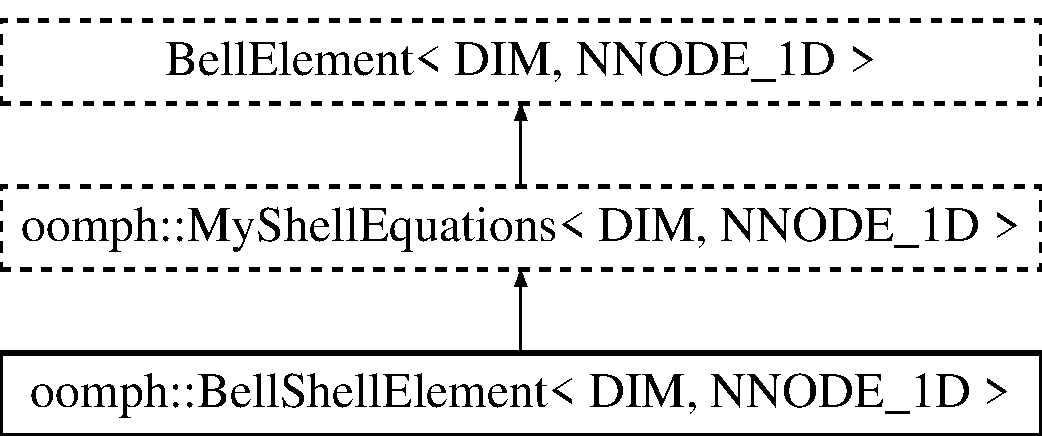
\includegraphics[height=3.000000cm]{classoomph_1_1BellShellElement}
\end{center}
\end{figure}
\subsection*{Public Member Functions}
\begin{DoxyCompactItemize}
\item 
\hyperlink{classoomph_1_1BellShellElement_a9c8946b0c97fc993db62acafc76301d8}{Bell\+Shell\+Element} ()
\begin{DoxyCompactList}\small\item\em Constructor\+: Call constructors for Bell\+Element and Shell equations. \end{DoxyCompactList}\item 
\hyperlink{classoomph_1_1BellShellElement_a9a3476e77088236068b559a7021a899d}{Bell\+Shell\+Element} (const \hyperlink{classoomph_1_1BellShellElement}{Bell\+Shell\+Element}$<$ D\+IM, N\+N\+O\+D\+E\+\_\+1D $>$ \&dummy)
\begin{DoxyCompactList}\small\item\em Broken copy constructor. \end{DoxyCompactList}\item 
unsigned \hyperlink{classoomph_1_1BellShellElement_aea6c22273ebe4a34111846313716fb0f}{required\+\_\+nvalue} (const unsigned \&n) const
\begin{DoxyCompactList}\small\item\em Required \# of `values\textquotesingle{} (pinned or dofs) at node n. \end{DoxyCompactList}\item 
void \hyperlink{classoomph_1_1BellShellElement_aebeebfbb5296217e3b6492392df3aeb5}{output} (std\+::ostream \&outfile)
\begin{DoxyCompactList}\small\item\em Output function\+: x,y,u or x,y,z,u. \end{DoxyCompactList}\item 
void \hyperlink{classoomph_1_1BellShellElement_a3bd16bf3ed27512990a593f8af97826d}{output} (std\+::ostream \&outfile, const unsigned \&n\+\_\+plot)
\begin{DoxyCompactList}\small\item\em Output function\+: x,y,u or x,y,z,u at n\+\_\+plot$^\wedge$\+D\+IM plot points. \end{DoxyCompactList}\item 
void \hyperlink{classoomph_1_1BellShellElement_a9abec4ec4338f67f88fcda4ff143e972}{output} (F\+I\+LE $\ast$file\+\_\+pt)
\begin{DoxyCompactList}\small\item\em C-\/style output function\+: x,y,u or x,y,z,u. \end{DoxyCompactList}\item 
void \hyperlink{classoomph_1_1BellShellElement_a6f203728a7d113a2b1029d18f7bff533}{output} (F\+I\+LE $\ast$file\+\_\+pt, const unsigned \&n\+\_\+plot)
\begin{DoxyCompactList}\small\item\em C-\/style output function\+: x,y,u or x,y,z,u at n\+\_\+plot$^\wedge$\+D\+IM plot points. \end{DoxyCompactList}\item 
void \hyperlink{classoomph_1_1BellShellElement_aaf6d152626e653db12f0d6d3c71b0fef}{output\+\_\+fct} (std\+::ostream \&outfile, const unsigned \&n\+\_\+plot, Finite\+Element\+::\+Steady\+Exact\+Solution\+Fct\+Pt exact\+\_\+soln\+\_\+pt)
\begin{DoxyCompactList}\small\item\em Output function for an exact solution\+: x,y,u\+\_\+exact or x,y,z,u\+\_\+exact at n\+\_\+plot$^\wedge$\+D\+IM plot points. \end{DoxyCompactList}\item 
void \hyperlink{classoomph_1_1BellShellElement_a5589f860978d78c64278afdbc72f5f5d}{output\+\_\+fct} (std\+::ostream \&outfile, const unsigned \&n\+\_\+plot, const double \&time, Finite\+Element\+::\+Unsteady\+Exact\+Solution\+Fct\+Pt exact\+\_\+soln\+\_\+pt)
\begin{DoxyCompactList}\small\item\em Output function for a time-\/dependent exact solution. x,y,u\+\_\+exact or x,y,z,u\+\_\+exact at n\+\_\+plot$^\wedge$\+D\+IM plot points (Calls the steady version) \end{DoxyCompactList}\end{DoxyCompactItemize}
\subsection*{Protected Member Functions}
\begin{DoxyCompactItemize}
\item 
double \hyperlink{classoomph_1_1BellShellElement_ace76c40d2ccff50c50140cb27ef9e6f6}{d2shape\+\_\+and\+\_\+d2test\+\_\+eulerian\+\_\+shell} (const Vector$<$ double $>$ \&s, Shape \&psi, D\+Shape \&dpsidx, D\+Shape \&d2psidx, Shape \&test, D\+Shape \&dtestdx, D\+Shape \&d2testdx) const
\begin{DoxyCompactList}\small\item\em Shape, test functions \& derivs. w.\+r.\+t. to global coords. Return Jacobian. \end{DoxyCompactList}\item 
double \hyperlink{classoomph_1_1BellShellElement_aab519c12f08b5a723d6eab3e1a0a3e84}{dshape\+\_\+and\+\_\+dtest\+\_\+eulerian\+\_\+shell} (const Vector$<$ double $>$ \&s, Shape \&psi, D\+Shape \&dpsidx, Shape \&test, D\+Shape \&dtestdx) const
\item 
double \hyperlink{classoomph_1_1BellShellElement_a00932feabc5283a7edbff0cf8c52eb67}{d2shape\+\_\+and\+\_\+d2test\+\_\+eulerian\+\_\+at\+\_\+knot\+\_\+shell} (const unsigned \&ipt, Shape \&psi, D\+Shape \&dpsidx, D\+Shape \&d2psidx, Shape \&test, D\+Shape \&dtestdx, D\+Shape \&d2testdx) const
\begin{DoxyCompactList}\small\item\em Shape, test functions \& derivs. w.\+r.\+t. to global coords. at integration point ipt. Return Jacobian. \end{DoxyCompactList}\item 
double \hyperlink{classoomph_1_1BellShellElement_a56fcbf1446e8797e3066c802140d5baf}{dshape\+\_\+and\+\_\+dtest\+\_\+eulerian\+\_\+at\+\_\+knot\+\_\+shell} (const unsigned \&ipt, Shape \&psi, D\+Shape \&dpsidx, Shape \&test, D\+Shape \&dtestdx) const
\end{DoxyCompactItemize}
\subsection*{Static Private Attributes}
\begin{DoxyCompactItemize}
\item 
static const unsigned \hyperlink{classoomph_1_1BellShellElement_a85143ad34e170cb267211069ee7e334f}{Initial\+\_\+\+Nvalue} = 8
\begin{DoxyCompactList}\small\item\em Static int that holds the number of variables at nodes\+: always the same. \end{DoxyCompactList}\end{DoxyCompactItemize}
\subsection*{Additional Inherited Members}


\subsection{Detailed Description}
\subsubsection*{template$<$unsigned D\+IM, unsigned N\+N\+O\+D\+E\+\_\+1D$>$\newline
class oomph\+::\+Bell\+Shell\+Element$<$ D\+I\+M, N\+N\+O\+D\+E\+\_\+1\+D $>$}

\hyperlink{classoomph_1_1BellShellElement}{Bell\+Shell\+Element} elements are with subparametric interpolation for the function. 

Definition at line 518 of file unstructured\+\_\+clamped\+\_\+square\+\_\+plate.\+cc.



\subsection{Constructor \& Destructor Documentation}
\mbox{\Hypertarget{classoomph_1_1BellShellElement_a9c8946b0c97fc993db62acafc76301d8}\label{classoomph_1_1BellShellElement_a9c8946b0c97fc993db62acafc76301d8}} 
\index{oomph\+::\+Bell\+Shell\+Element@{oomph\+::\+Bell\+Shell\+Element}!Bell\+Shell\+Element@{Bell\+Shell\+Element}}
\index{Bell\+Shell\+Element@{Bell\+Shell\+Element}!oomph\+::\+Bell\+Shell\+Element@{oomph\+::\+Bell\+Shell\+Element}}
\subsubsection{\texorpdfstring{Bell\+Shell\+Element()}{BellShellElement()}\hspace{0.1cm}{\footnotesize\ttfamily [1/2]}}
{\footnotesize\ttfamily template$<$unsigned D\+IM, unsigned N\+N\+O\+D\+E\+\_\+1D$>$ \\
\hyperlink{classoomph_1_1BellShellElement}{oomph\+::\+Bell\+Shell\+Element}$<$ D\+IM, N\+N\+O\+D\+E\+\_\+1D $>$\+::\hyperlink{classoomph_1_1BellShellElement}{Bell\+Shell\+Element} (\begin{DoxyParamCaption}{ }\end{DoxyParamCaption})\hspace{0.3cm}{\ttfamily [inline]}}



Constructor\+: Call constructors for Bell\+Element and Shell equations. 



Definition at line 532 of file unstructured\+\_\+clamped\+\_\+square\+\_\+plate.\+cc.

\mbox{\Hypertarget{classoomph_1_1BellShellElement_a9a3476e77088236068b559a7021a899d}\label{classoomph_1_1BellShellElement_a9a3476e77088236068b559a7021a899d}} 
\index{oomph\+::\+Bell\+Shell\+Element@{oomph\+::\+Bell\+Shell\+Element}!Bell\+Shell\+Element@{Bell\+Shell\+Element}}
\index{Bell\+Shell\+Element@{Bell\+Shell\+Element}!oomph\+::\+Bell\+Shell\+Element@{oomph\+::\+Bell\+Shell\+Element}}
\subsubsection{\texorpdfstring{Bell\+Shell\+Element()}{BellShellElement()}\hspace{0.1cm}{\footnotesize\ttfamily [2/2]}}
{\footnotesize\ttfamily template$<$unsigned D\+IM, unsigned N\+N\+O\+D\+E\+\_\+1D$>$ \\
\hyperlink{classoomph_1_1BellShellElement}{oomph\+::\+Bell\+Shell\+Element}$<$ D\+IM, N\+N\+O\+D\+E\+\_\+1D $>$\+::\hyperlink{classoomph_1_1BellShellElement}{Bell\+Shell\+Element} (\begin{DoxyParamCaption}\item[{const \hyperlink{classoomph_1_1BellShellElement}{Bell\+Shell\+Element}$<$ D\+IM, N\+N\+O\+D\+E\+\_\+1D $>$ \&}]{dummy }\end{DoxyParamCaption})\hspace{0.3cm}{\ttfamily [inline]}}



Broken copy constructor. 



Definition at line 536 of file unstructured\+\_\+clamped\+\_\+square\+\_\+plate.\+cc.



\subsection{Member Function Documentation}
\mbox{\Hypertarget{classoomph_1_1BellShellElement_a00932feabc5283a7edbff0cf8c52eb67}\label{classoomph_1_1BellShellElement_a00932feabc5283a7edbff0cf8c52eb67}} 
\index{oomph\+::\+Bell\+Shell\+Element@{oomph\+::\+Bell\+Shell\+Element}!d2shape\+\_\+and\+\_\+d2test\+\_\+eulerian\+\_\+at\+\_\+knot\+\_\+shell@{d2shape\+\_\+and\+\_\+d2test\+\_\+eulerian\+\_\+at\+\_\+knot\+\_\+shell}}
\index{d2shape\+\_\+and\+\_\+d2test\+\_\+eulerian\+\_\+at\+\_\+knot\+\_\+shell@{d2shape\+\_\+and\+\_\+d2test\+\_\+eulerian\+\_\+at\+\_\+knot\+\_\+shell}!oomph\+::\+Bell\+Shell\+Element@{oomph\+::\+Bell\+Shell\+Element}}
\subsubsection{\texorpdfstring{d2shape\+\_\+and\+\_\+d2test\+\_\+eulerian\+\_\+at\+\_\+knot\+\_\+shell()}{d2shape\_and\_d2test\_eulerian\_at\_knot\_shell()}}
{\footnotesize\ttfamily template$<$unsigned D\+IM, unsigned N\+N\+O\+D\+E\+\_\+1D$>$ \\
double \hyperlink{classoomph_1_1BellShellElement}{oomph\+::\+Bell\+Shell\+Element}$<$ D\+IM, N\+N\+O\+D\+E\+\_\+1D $>$\+::d2shape\+\_\+and\+\_\+d2test\+\_\+eulerian\+\_\+at\+\_\+knot\+\_\+shell (\begin{DoxyParamCaption}\item[{const unsigned \&}]{ipt,  }\item[{Shape \&}]{psi,  }\item[{D\+Shape \&}]{dpsidx,  }\item[{D\+Shape \&}]{d2psidx,  }\item[{Shape \&}]{test,  }\item[{D\+Shape \&}]{dtestdx,  }\item[{D\+Shape \&}]{d2testdx }\end{DoxyParamCaption}) const\hspace{0.3cm}{\ttfamily [inline]}, {\ttfamily [protected]}, {\ttfamily [virtual]}}



Shape, test functions \& derivs. w.\+r.\+t. to global coords. at integration point ipt. Return Jacobian. 



Implements \hyperlink{classoomph_1_1MyShellEquations_af8f15f0d678c85535bbc3390399dafdd}{oomph\+::\+My\+Shell\+Equations$<$ D\+I\+M, N\+N\+O\+D\+E\+\_\+1\+D $>$}.



Definition at line 715 of file unstructured\+\_\+clamped\+\_\+square\+\_\+plate.\+cc.

\mbox{\Hypertarget{classoomph_1_1BellShellElement_ace76c40d2ccff50c50140cb27ef9e6f6}\label{classoomph_1_1BellShellElement_ace76c40d2ccff50c50140cb27ef9e6f6}} 
\index{oomph\+::\+Bell\+Shell\+Element@{oomph\+::\+Bell\+Shell\+Element}!d2shape\+\_\+and\+\_\+d2test\+\_\+eulerian\+\_\+shell@{d2shape\+\_\+and\+\_\+d2test\+\_\+eulerian\+\_\+shell}}
\index{d2shape\+\_\+and\+\_\+d2test\+\_\+eulerian\+\_\+shell@{d2shape\+\_\+and\+\_\+d2test\+\_\+eulerian\+\_\+shell}!oomph\+::\+Bell\+Shell\+Element@{oomph\+::\+Bell\+Shell\+Element}}
\subsubsection{\texorpdfstring{d2shape\+\_\+and\+\_\+d2test\+\_\+eulerian\+\_\+shell()}{d2shape\_and\_d2test\_eulerian\_shell()}}
{\footnotesize\ttfamily template$<$unsigned D\+IM, unsigned N\+N\+O\+D\+E\+\_\+1D$>$ \\
double \hyperlink{classoomph_1_1BellShellElement}{oomph\+::\+Bell\+Shell\+Element}$<$ D\+IM, N\+N\+O\+D\+E\+\_\+1D $>$\+::d2shape\+\_\+and\+\_\+d2test\+\_\+eulerian\+\_\+shell (\begin{DoxyParamCaption}\item[{const Vector$<$ double $>$ \&}]{s,  }\item[{Shape \&}]{psi,  }\item[{D\+Shape \&}]{dpsidx,  }\item[{D\+Shape \&}]{d2psidx,  }\item[{Shape \&}]{test,  }\item[{D\+Shape \&}]{dtestdx,  }\item[{D\+Shape \&}]{d2testdx }\end{DoxyParamCaption}) const\hspace{0.3cm}{\ttfamily [inline]}, {\ttfamily [protected]}, {\ttfamily [virtual]}}



Shape, test functions \& derivs. w.\+r.\+t. to global coords. Return Jacobian. 



Implements \hyperlink{classoomph_1_1MyShellEquations_ae5efd29cb214218d41d29abab4dcec51}{oomph\+::\+My\+Shell\+Equations$<$ D\+I\+M, N\+N\+O\+D\+E\+\_\+1\+D $>$}.



Definition at line 669 of file unstructured\+\_\+clamped\+\_\+square\+\_\+plate.\+cc.

\mbox{\Hypertarget{classoomph_1_1BellShellElement_a56fcbf1446e8797e3066c802140d5baf}\label{classoomph_1_1BellShellElement_a56fcbf1446e8797e3066c802140d5baf}} 
\index{oomph\+::\+Bell\+Shell\+Element@{oomph\+::\+Bell\+Shell\+Element}!dshape\+\_\+and\+\_\+dtest\+\_\+eulerian\+\_\+at\+\_\+knot\+\_\+shell@{dshape\+\_\+and\+\_\+dtest\+\_\+eulerian\+\_\+at\+\_\+knot\+\_\+shell}}
\index{dshape\+\_\+and\+\_\+dtest\+\_\+eulerian\+\_\+at\+\_\+knot\+\_\+shell@{dshape\+\_\+and\+\_\+dtest\+\_\+eulerian\+\_\+at\+\_\+knot\+\_\+shell}!oomph\+::\+Bell\+Shell\+Element@{oomph\+::\+Bell\+Shell\+Element}}
\subsubsection{\texorpdfstring{dshape\+\_\+and\+\_\+dtest\+\_\+eulerian\+\_\+at\+\_\+knot\+\_\+shell()}{dshape\_and\_dtest\_eulerian\_at\_knot\_shell()}}
{\footnotesize\ttfamily template$<$unsigned D\+IM, unsigned N\+N\+O\+D\+E\+\_\+1D$>$ \\
double \hyperlink{classoomph_1_1BellShellElement}{oomph\+::\+Bell\+Shell\+Element}$<$ D\+IM, N\+N\+O\+D\+E\+\_\+1D $>$\+::dshape\+\_\+and\+\_\+dtest\+\_\+eulerian\+\_\+at\+\_\+knot\+\_\+shell (\begin{DoxyParamCaption}\item[{const unsigned \&}]{ipt,  }\item[{Shape \&}]{psi,  }\item[{D\+Shape \&}]{dpsidx,  }\item[{Shape \&}]{test,  }\item[{D\+Shape \&}]{dtestdx }\end{DoxyParamCaption}) const\hspace{0.3cm}{\ttfamily [inline]}, {\ttfamily [protected]}, {\ttfamily [virtual]}}

Define the shape functions and test functions and derivatives w.\+r.\+t. global coordinates and return Jacobian of mapping.

Galerkin\+: Test functions = shape functions 

Implements \hyperlink{classoomph_1_1MyShellEquations_a0800ff2f9716a3b0327624948ce792e1}{oomph\+::\+My\+Shell\+Equations$<$ D\+I\+M, N\+N\+O\+D\+E\+\_\+1\+D $>$}.



Definition at line 701 of file unstructured\+\_\+clamped\+\_\+square\+\_\+plate.\+cc.

\mbox{\Hypertarget{classoomph_1_1BellShellElement_aab519c12f08b5a723d6eab3e1a0a3e84}\label{classoomph_1_1BellShellElement_aab519c12f08b5a723d6eab3e1a0a3e84}} 
\index{oomph\+::\+Bell\+Shell\+Element@{oomph\+::\+Bell\+Shell\+Element}!dshape\+\_\+and\+\_\+dtest\+\_\+eulerian\+\_\+shell@{dshape\+\_\+and\+\_\+dtest\+\_\+eulerian\+\_\+shell}}
\index{dshape\+\_\+and\+\_\+dtest\+\_\+eulerian\+\_\+shell@{dshape\+\_\+and\+\_\+dtest\+\_\+eulerian\+\_\+shell}!oomph\+::\+Bell\+Shell\+Element@{oomph\+::\+Bell\+Shell\+Element}}
\subsubsection{\texorpdfstring{dshape\+\_\+and\+\_\+dtest\+\_\+eulerian\+\_\+shell()}{dshape\_and\_dtest\_eulerian\_shell()}}
{\footnotesize\ttfamily template$<$unsigned D\+IM, unsigned N\+N\+O\+D\+E\+\_\+1D$>$ \\
double \hyperlink{classoomph_1_1BellShellElement}{oomph\+::\+Bell\+Shell\+Element}$<$ D\+IM, N\+N\+O\+D\+E\+\_\+1D $>$\+::dshape\+\_\+and\+\_\+dtest\+\_\+eulerian\+\_\+shell (\begin{DoxyParamCaption}\item[{const Vector$<$ double $>$ \&}]{s,  }\item[{Shape \&}]{psi,  }\item[{D\+Shape \&}]{dpsidx,  }\item[{Shape \&}]{test,  }\item[{D\+Shape \&}]{dtestdx }\end{DoxyParamCaption}) const\hspace{0.3cm}{\ttfamily [inline]}, {\ttfamily [protected]}, {\ttfamily [virtual]}}

Define the shape functions and test functions and derivatives w.\+r.\+t. global coordinates and return Jacobian of mapping.

Galerkin\+: Test functions = shape functions 

Implements \hyperlink{classoomph_1_1MyShellEquations_ac0cb5a90f9eceb2406c21c1e1dc662e7}{oomph\+::\+My\+Shell\+Equations$<$ D\+I\+M, N\+N\+O\+D\+E\+\_\+1\+D $>$}.



Definition at line 655 of file unstructured\+\_\+clamped\+\_\+square\+\_\+plate.\+cc.

\mbox{\Hypertarget{classoomph_1_1BellShellElement_aebeebfbb5296217e3b6492392df3aeb5}\label{classoomph_1_1BellShellElement_aebeebfbb5296217e3b6492392df3aeb5}} 
\index{oomph\+::\+Bell\+Shell\+Element@{oomph\+::\+Bell\+Shell\+Element}!output@{output}}
\index{output@{output}!oomph\+::\+Bell\+Shell\+Element@{oomph\+::\+Bell\+Shell\+Element}}
\subsubsection{\texorpdfstring{output()}{output()}\hspace{0.1cm}{\footnotesize\ttfamily [1/4]}}
{\footnotesize\ttfamily template$<$unsigned D\+IM, unsigned N\+N\+O\+D\+E\+\_\+1D$>$ \\
void \hyperlink{classoomph_1_1BellShellElement}{oomph\+::\+Bell\+Shell\+Element}$<$ D\+IM, N\+N\+O\+D\+E\+\_\+1D $>$\+::output (\begin{DoxyParamCaption}\item[{std\+::ostream \&}]{outfile }\end{DoxyParamCaption})\hspace{0.3cm}{\ttfamily [inline]}}



Output function\+: x,y,u or x,y,z,u. 



Definition at line 549 of file unstructured\+\_\+clamped\+\_\+square\+\_\+plate.\+cc.

\mbox{\Hypertarget{classoomph_1_1BellShellElement_a3bd16bf3ed27512990a593f8af97826d}\label{classoomph_1_1BellShellElement_a3bd16bf3ed27512990a593f8af97826d}} 
\index{oomph\+::\+Bell\+Shell\+Element@{oomph\+::\+Bell\+Shell\+Element}!output@{output}}
\index{output@{output}!oomph\+::\+Bell\+Shell\+Element@{oomph\+::\+Bell\+Shell\+Element}}
\subsubsection{\texorpdfstring{output()}{output()}\hspace{0.1cm}{\footnotesize\ttfamily [2/4]}}
{\footnotesize\ttfamily template$<$unsigned D\+IM, unsigned N\+N\+O\+D\+E\+\_\+1D$>$ \\
void \hyperlink{classoomph_1_1BellShellElement}{oomph\+::\+Bell\+Shell\+Element}$<$ D\+IM, N\+N\+O\+D\+E\+\_\+1D $>$\+::output (\begin{DoxyParamCaption}\item[{std\+::ostream \&}]{outfile,  }\item[{const unsigned \&}]{n\+\_\+plot }\end{DoxyParamCaption})\hspace{0.3cm}{\ttfamily [inline]}}



Output function\+: x,y,u or x,y,z,u at n\+\_\+plot$^\wedge$\+D\+IM plot points. 



Definition at line 555 of file unstructured\+\_\+clamped\+\_\+square\+\_\+plate.\+cc.

\mbox{\Hypertarget{classoomph_1_1BellShellElement_a9abec4ec4338f67f88fcda4ff143e972}\label{classoomph_1_1BellShellElement_a9abec4ec4338f67f88fcda4ff143e972}} 
\index{oomph\+::\+Bell\+Shell\+Element@{oomph\+::\+Bell\+Shell\+Element}!output@{output}}
\index{output@{output}!oomph\+::\+Bell\+Shell\+Element@{oomph\+::\+Bell\+Shell\+Element}}
\subsubsection{\texorpdfstring{output()}{output()}\hspace{0.1cm}{\footnotesize\ttfamily [3/4]}}
{\footnotesize\ttfamily template$<$unsigned D\+IM, unsigned N\+N\+O\+D\+E\+\_\+1D$>$ \\
void \hyperlink{classoomph_1_1BellShellElement}{oomph\+::\+Bell\+Shell\+Element}$<$ D\+IM, N\+N\+O\+D\+E\+\_\+1D $>$\+::output (\begin{DoxyParamCaption}\item[{F\+I\+LE $\ast$}]{file\+\_\+pt }\end{DoxyParamCaption})\hspace{0.3cm}{\ttfamily [inline]}}



C-\/style output function\+: x,y,u or x,y,z,u. 



Definition at line 561 of file unstructured\+\_\+clamped\+\_\+square\+\_\+plate.\+cc.

\mbox{\Hypertarget{classoomph_1_1BellShellElement_a6f203728a7d113a2b1029d18f7bff533}\label{classoomph_1_1BellShellElement_a6f203728a7d113a2b1029d18f7bff533}} 
\index{oomph\+::\+Bell\+Shell\+Element@{oomph\+::\+Bell\+Shell\+Element}!output@{output}}
\index{output@{output}!oomph\+::\+Bell\+Shell\+Element@{oomph\+::\+Bell\+Shell\+Element}}
\subsubsection{\texorpdfstring{output()}{output()}\hspace{0.1cm}{\footnotesize\ttfamily [4/4]}}
{\footnotesize\ttfamily template$<$unsigned D\+IM, unsigned N\+N\+O\+D\+E\+\_\+1D$>$ \\
void \hyperlink{classoomph_1_1BellShellElement}{oomph\+::\+Bell\+Shell\+Element}$<$ D\+IM, N\+N\+O\+D\+E\+\_\+1D $>$\+::output (\begin{DoxyParamCaption}\item[{F\+I\+LE $\ast$}]{file\+\_\+pt,  }\item[{const unsigned \&}]{n\+\_\+plot }\end{DoxyParamCaption})\hspace{0.3cm}{\ttfamily [inline]}}



C-\/style output function\+: x,y,u or x,y,z,u at n\+\_\+plot$^\wedge$\+D\+IM plot points. 



Definition at line 567 of file unstructured\+\_\+clamped\+\_\+square\+\_\+plate.\+cc.

\mbox{\Hypertarget{classoomph_1_1BellShellElement_aaf6d152626e653db12f0d6d3c71b0fef}\label{classoomph_1_1BellShellElement_aaf6d152626e653db12f0d6d3c71b0fef}} 
\index{oomph\+::\+Bell\+Shell\+Element@{oomph\+::\+Bell\+Shell\+Element}!output\+\_\+fct@{output\+\_\+fct}}
\index{output\+\_\+fct@{output\+\_\+fct}!oomph\+::\+Bell\+Shell\+Element@{oomph\+::\+Bell\+Shell\+Element}}
\subsubsection{\texorpdfstring{output\+\_\+fct()}{output\_fct()}\hspace{0.1cm}{\footnotesize\ttfamily [1/2]}}
{\footnotesize\ttfamily template$<$unsigned D\+IM, unsigned N\+N\+O\+D\+E\+\_\+1D$>$ \\
void \hyperlink{classoomph_1_1BellShellElement}{oomph\+::\+Bell\+Shell\+Element}$<$ D\+IM, N\+N\+O\+D\+E\+\_\+1D $>$\+::output\+\_\+fct (\begin{DoxyParamCaption}\item[{std\+::ostream \&}]{outfile,  }\item[{const unsigned \&}]{n\+\_\+plot,  }\item[{Finite\+Element\+::\+Steady\+Exact\+Solution\+Fct\+Pt}]{exact\+\_\+soln\+\_\+pt }\end{DoxyParamCaption})\hspace{0.3cm}{\ttfamily [inline]}}



Output function for an exact solution\+: x,y,u\+\_\+exact or x,y,z,u\+\_\+exact at n\+\_\+plot$^\wedge$\+D\+IM plot points. 



Definition at line 573 of file unstructured\+\_\+clamped\+\_\+square\+\_\+plate.\+cc.

\mbox{\Hypertarget{classoomph_1_1BellShellElement_a5589f860978d78c64278afdbc72f5f5d}\label{classoomph_1_1BellShellElement_a5589f860978d78c64278afdbc72f5f5d}} 
\index{oomph\+::\+Bell\+Shell\+Element@{oomph\+::\+Bell\+Shell\+Element}!output\+\_\+fct@{output\+\_\+fct}}
\index{output\+\_\+fct@{output\+\_\+fct}!oomph\+::\+Bell\+Shell\+Element@{oomph\+::\+Bell\+Shell\+Element}}
\subsubsection{\texorpdfstring{output\+\_\+fct()}{output\_fct()}\hspace{0.1cm}{\footnotesize\ttfamily [2/2]}}
{\footnotesize\ttfamily template$<$unsigned D\+IM, unsigned N\+N\+O\+D\+E\+\_\+1D$>$ \\
void \hyperlink{classoomph_1_1BellShellElement}{oomph\+::\+Bell\+Shell\+Element}$<$ D\+IM, N\+N\+O\+D\+E\+\_\+1D $>$\+::output\+\_\+fct (\begin{DoxyParamCaption}\item[{std\+::ostream \&}]{outfile,  }\item[{const unsigned \&}]{n\+\_\+plot,  }\item[{const double \&}]{time,  }\item[{Finite\+Element\+::\+Unsteady\+Exact\+Solution\+Fct\+Pt}]{exact\+\_\+soln\+\_\+pt }\end{DoxyParamCaption})\hspace{0.3cm}{\ttfamily [inline]}, {\ttfamily [virtual]}}



Output function for a time-\/dependent exact solution. x,y,u\+\_\+exact or x,y,z,u\+\_\+exact at n\+\_\+plot$^\wedge$\+D\+IM plot points (Calls the steady version) 



Reimplemented from \hyperlink{classoomph_1_1MyShellEquations_a7022e91eaf4bff9044e46549bbe0c3f5}{oomph\+::\+My\+Shell\+Equations$<$ D\+I\+M, N\+N\+O\+D\+E\+\_\+1\+D $>$}.



Definition at line 582 of file unstructured\+\_\+clamped\+\_\+square\+\_\+plate.\+cc.

\mbox{\Hypertarget{classoomph_1_1BellShellElement_aea6c22273ebe4a34111846313716fb0f}\label{classoomph_1_1BellShellElement_aea6c22273ebe4a34111846313716fb0f}} 
\index{oomph\+::\+Bell\+Shell\+Element@{oomph\+::\+Bell\+Shell\+Element}!required\+\_\+nvalue@{required\+\_\+nvalue}}
\index{required\+\_\+nvalue@{required\+\_\+nvalue}!oomph\+::\+Bell\+Shell\+Element@{oomph\+::\+Bell\+Shell\+Element}}
\subsubsection{\texorpdfstring{required\+\_\+nvalue()}{required\_nvalue()}}
{\footnotesize\ttfamily template$<$unsigned D\+IM, unsigned N\+N\+O\+D\+E\+\_\+1D$>$ \\
unsigned \hyperlink{classoomph_1_1BellShellElement}{oomph\+::\+Bell\+Shell\+Element}$<$ D\+IM, N\+N\+O\+D\+E\+\_\+1D $>$\+::required\+\_\+nvalue (\begin{DoxyParamCaption}\item[{const unsigned \&}]{n }\end{DoxyParamCaption}) const\hspace{0.3cm}{\ttfamily [inline]}}



Required \# of `values\textquotesingle{} (pinned or dofs) at node n. 



Definition at line 544 of file unstructured\+\_\+clamped\+\_\+square\+\_\+plate.\+cc.



\subsection{Member Data Documentation}
\mbox{\Hypertarget{classoomph_1_1BellShellElement_a85143ad34e170cb267211069ee7e334f}\label{classoomph_1_1BellShellElement_a85143ad34e170cb267211069ee7e334f}} 
\index{oomph\+::\+Bell\+Shell\+Element@{oomph\+::\+Bell\+Shell\+Element}!Initial\+\_\+\+Nvalue@{Initial\+\_\+\+Nvalue}}
\index{Initial\+\_\+\+Nvalue@{Initial\+\_\+\+Nvalue}!oomph\+::\+Bell\+Shell\+Element@{oomph\+::\+Bell\+Shell\+Element}}
\subsubsection{\texorpdfstring{Initial\+\_\+\+Nvalue}{Initial\_Nvalue}}
{\footnotesize\ttfamily template$<$unsigned D\+IM, unsigned N\+N\+O\+D\+E\+\_\+1D$>$ \\
const unsigned \hyperlink{classoomph_1_1BellShellElement}{oomph\+::\+Bell\+Shell\+Element}$<$ D\+IM, N\+N\+O\+D\+E\+\_\+1D $>$\+::Initial\+\_\+\+Nvalue = 8\hspace{0.3cm}{\ttfamily [static]}, {\ttfamily [private]}}



Static int that holds the number of variables at nodes\+: always the same. 

Set the data for the number of Variables at each node. 

Definition at line 525 of file unstructured\+\_\+clamped\+\_\+square\+\_\+plate.\+cc.



The documentation for this class was generated from the following file\+:\begin{DoxyCompactItemize}
\item 
\hyperlink{unstructured__clamped__square__plate_8cc}{unstructured\+\_\+clamped\+\_\+square\+\_\+plate.\+cc}\end{DoxyCompactItemize}

\hypertarget{classoomph_1_1FaceGeometry_3_01BellShellElement_3_01DIM_00_01NNODE__1D_01_4_01_4}{}\section{oomph\+:\+:Face\+Geometry$<$ Bell\+Shell\+Element$<$ D\+IM, N\+N\+O\+D\+E\+\_\+1D $>$ $>$ Class Template Reference}
\label{classoomph_1_1FaceGeometry_3_01BellShellElement_3_01DIM_00_01NNODE__1D_01_4_01_4}\index{oomph\+::\+Face\+Geometry$<$ Bell\+Shell\+Element$<$ D\+I\+M, N\+N\+O\+D\+E\+\_\+1\+D $>$ $>$@{oomph\+::\+Face\+Geometry$<$ Bell\+Shell\+Element$<$ D\+I\+M, N\+N\+O\+D\+E\+\_\+1\+D $>$ $>$}}
Inheritance diagram for oomph\+:\+:Face\+Geometry$<$ Bell\+Shell\+Element$<$ D\+IM, N\+N\+O\+D\+E\+\_\+1D $>$ $>$\+:\begin{figure}[H]
\begin{center}
\leavevmode
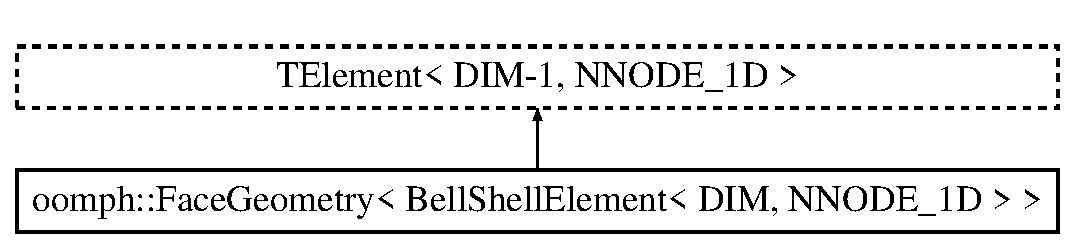
\includegraphics[height=2.000000cm]{classoomph_1_1FaceGeometry_3_01BellShellElement_3_01DIM_00_01NNODE__1D_01_4_01_4}
\end{center}
\end{figure}
\subsection*{Public Member Functions}
\begin{DoxyCompactItemize}
\item 
\hyperlink{classoomph_1_1FaceGeometry_3_01BellShellElement_3_01DIM_00_01NNODE__1D_01_4_01_4_ae3b9e81d2729d8b818c563812e8cf8f9}{Face\+Geometry} ()
\begin{DoxyCompactList}\small\item\em Constructor\+: Call the constructor for the appropriate lower-\/dimensional T\+Element. \end{DoxyCompactList}\end{DoxyCompactItemize}


\subsection{Detailed Description}
\subsubsection*{template$<$unsigned D\+IM, unsigned N\+N\+O\+D\+E\+\_\+1D$>$\newline
class oomph\+::\+Face\+Geometry$<$ Bell\+Shell\+Element$<$ D\+I\+M, N\+N\+O\+D\+E\+\_\+1\+D $>$ $>$}

Face geometry for the \hyperlink{classoomph_1_1BellShellElement}{Bell\+Shell\+Element} elements\+: The spatial dimension of the face elements is one lower than that of the bulk element but they have the same number of points along their 1D edges. 

Definition at line 521 of file unstructured\+\_\+clamped\+\_\+curved\+\_\+shell.\+cc.



\subsection{Constructor \& Destructor Documentation}
\mbox{\Hypertarget{classoomph_1_1FaceGeometry_3_01BellShellElement_3_01DIM_00_01NNODE__1D_01_4_01_4_ae3b9e81d2729d8b818c563812e8cf8f9}\label{classoomph_1_1FaceGeometry_3_01BellShellElement_3_01DIM_00_01NNODE__1D_01_4_01_4_ae3b9e81d2729d8b818c563812e8cf8f9}} 
\index{oomph\+::\+Face\+Geometry$<$ Bell\+Shell\+Element$<$ D\+I\+M, N\+N\+O\+D\+E\+\_\+1\+D $>$ $>$@{oomph\+::\+Face\+Geometry$<$ Bell\+Shell\+Element$<$ D\+I\+M, N\+N\+O\+D\+E\+\_\+1\+D $>$ $>$}!Face\+Geometry@{Face\+Geometry}}
\index{Face\+Geometry@{Face\+Geometry}!oomph\+::\+Face\+Geometry$<$ Bell\+Shell\+Element$<$ D\+I\+M, N\+N\+O\+D\+E\+\_\+1\+D $>$ $>$@{oomph\+::\+Face\+Geometry$<$ Bell\+Shell\+Element$<$ D\+I\+M, N\+N\+O\+D\+E\+\_\+1\+D $>$ $>$}}
\subsubsection{\texorpdfstring{Face\+Geometry()}{FaceGeometry()}}
{\footnotesize\ttfamily template$<$unsigned D\+IM, unsigned N\+N\+O\+D\+E\+\_\+1D$>$ \\
oomph\+::\+Face\+Geometry$<$ \hyperlink{classoomph_1_1BellShellElement}{Bell\+Shell\+Element}$<$ D\+IM, N\+N\+O\+D\+E\+\_\+1D $>$ $>$\+::Face\+Geometry (\begin{DoxyParamCaption}{ }\end{DoxyParamCaption})\hspace{0.3cm}{\ttfamily [inline]}}



Constructor\+: Call the constructor for the appropriate lower-\/dimensional T\+Element. 



Definition at line 529 of file unstructured\+\_\+clamped\+\_\+curved\+\_\+shell.\+cc.



The documentation for this class was generated from the following file\+:\begin{DoxyCompactItemize}
\item 
\hyperlink{unstructured__clamped__curved__shell_8cc}{unstructured\+\_\+clamped\+\_\+curved\+\_\+shell.\+cc}\end{DoxyCompactItemize}

\hypertarget{classFlatPlate}{}\section{Flat\+Plate Class Reference}
\label{classFlatPlate}\index{Flat\+Plate@{Flat\+Plate}}


Flat plate in x-\/y plane.  


Inheritance diagram for Flat\+Plate\+:\begin{figure}[H]
\begin{center}
\leavevmode
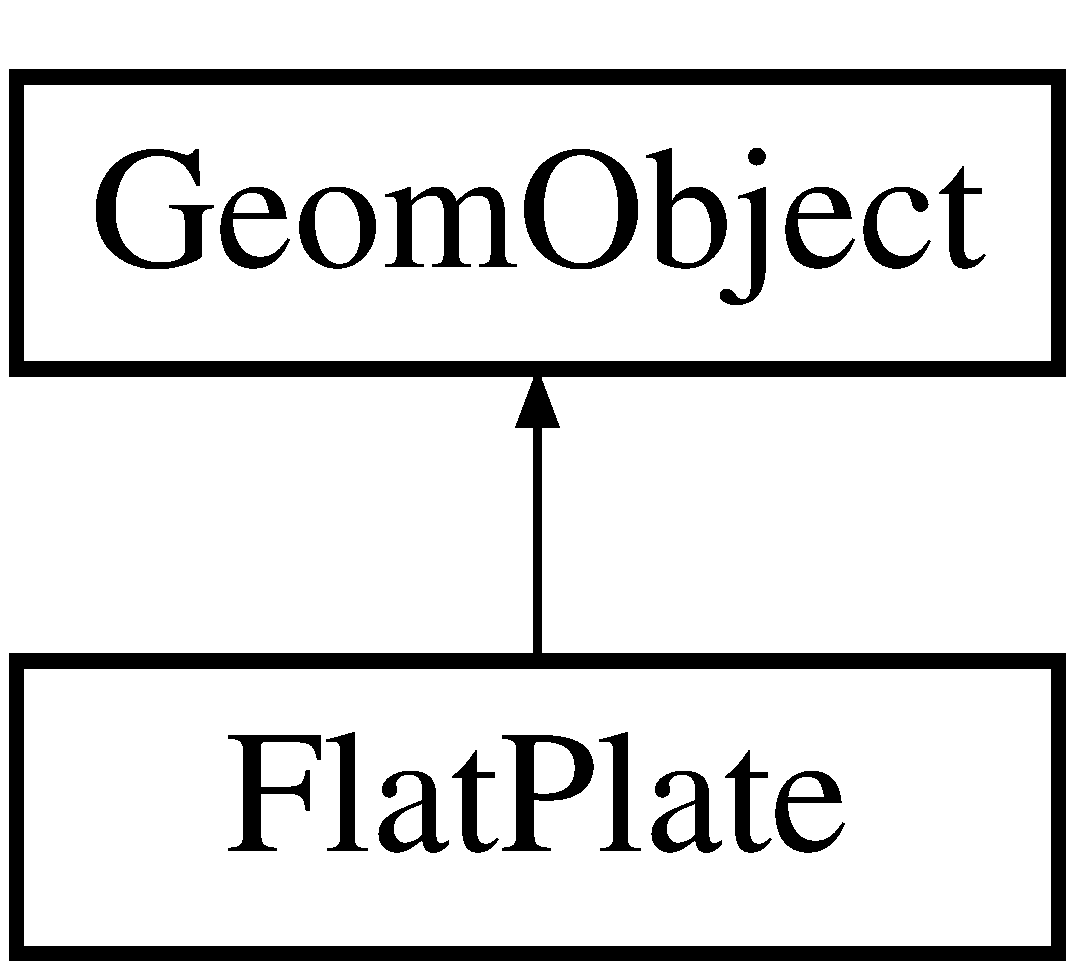
\includegraphics[height=2.000000cm]{classFlatPlate}
\end{center}
\end{figure}
\subsection*{Public Member Functions}
\begin{DoxyCompactItemize}
\item 
\hyperlink{classFlatPlate_a5a0e45f57f8d40885e220349aa1beaa6}{Flat\+Plate} ()
\begin{DoxyCompactList}\small\item\em Constructor\+: \end{DoxyCompactList}\item 
\hyperlink{classFlatPlate_a8d235775f64d0241d8111d3a743e1b49}{Flat\+Plate} (const \hyperlink{classFlatPlate}{Flat\+Plate} \&node)
\begin{DoxyCompactList}\small\item\em Broken copy constructor. \end{DoxyCompactList}\item 
void \hyperlink{classFlatPlate_af1ecfd0cc5b23be30488c8493ada6b2d}{operator=} (const \hyperlink{classFlatPlate}{Flat\+Plate} \&)
\begin{DoxyCompactList}\small\item\em Broken assignment operator. \end{DoxyCompactList}\item 
void \hyperlink{classFlatPlate_a4a8965c0578bbce8e56f174ae4590012}{position} (const Vector$<$ double $>$ \&zeta, Vector$<$ double $>$ \&r) const
\begin{DoxyCompactList}\small\item\em Position vector. \end{DoxyCompactList}\item 
void \hyperlink{classFlatPlate_ae5e3e3fcf6b8c412865a02a27aeeeaf0}{position} (const unsigned \&t, const Vector$<$ double $>$ \&zeta, Vector$<$ double $>$ \&r) const
\begin{DoxyCompactList}\small\item\em Position vector (dummy unsteady version returns steady version) \end{DoxyCompactList}\item 
virtual unsigned \hyperlink{classFlatPlate_ae7132e6fbbabf5543df743024b2ba9f7}{ngeom\+\_\+data} () const
\begin{DoxyCompactList}\small\item\em How many items of Data does the shape of the object depend on? \end{DoxyCompactList}\item 
void \hyperlink{classFlatPlate_a2c14c32689795ee19c5dfeb0026c5ec0}{d2position} (const Vector$<$ double $>$ \&zeta, Vector$<$ double $>$ \&r, Dense\+Matrix$<$ double $>$ \&drdzeta, Rank\+Three\+Tensor$<$ double $>$ \&ddrdzeta) const
\begin{DoxyCompactList}\small\item\em Position Vector and 1st and 2nd derivs w.\+r.\+t. zeta. \end{DoxyCompactList}\end{DoxyCompactItemize}


\subsection{Detailed Description}
Flat plate in x-\/y plane. 

Definition at line 54 of file plate.\+cc.



\subsection{Constructor \& Destructor Documentation}
\mbox{\Hypertarget{classFlatPlate_a5a0e45f57f8d40885e220349aa1beaa6}\label{classFlatPlate_a5a0e45f57f8d40885e220349aa1beaa6}} 
\index{Flat\+Plate@{Flat\+Plate}!Flat\+Plate@{Flat\+Plate}}
\index{Flat\+Plate@{Flat\+Plate}!Flat\+Plate@{Flat\+Plate}}
\subsubsection{\texorpdfstring{Flat\+Plate()}{FlatPlate()}\hspace{0.1cm}{\footnotesize\ttfamily [1/2]}}
{\footnotesize\ttfamily Flat\+Plate\+::\+Flat\+Plate (\begin{DoxyParamCaption}{ }\end{DoxyParamCaption})\hspace{0.3cm}{\ttfamily [inline]}}



Constructor\+: 



Definition at line 59 of file plate.\+cc.

\mbox{\Hypertarget{classFlatPlate_a8d235775f64d0241d8111d3a743e1b49}\label{classFlatPlate_a8d235775f64d0241d8111d3a743e1b49}} 
\index{Flat\+Plate@{Flat\+Plate}!Flat\+Plate@{Flat\+Plate}}
\index{Flat\+Plate@{Flat\+Plate}!Flat\+Plate@{Flat\+Plate}}
\subsubsection{\texorpdfstring{Flat\+Plate()}{FlatPlate()}\hspace{0.1cm}{\footnotesize\ttfamily [2/2]}}
{\footnotesize\ttfamily Flat\+Plate\+::\+Flat\+Plate (\begin{DoxyParamCaption}\item[{const \hyperlink{classFlatPlate}{Flat\+Plate} \&}]{node }\end{DoxyParamCaption})\hspace{0.3cm}{\ttfamily [inline]}}



Broken copy constructor. 



Definition at line 62 of file plate.\+cc.



\subsection{Member Function Documentation}
\mbox{\Hypertarget{classFlatPlate_a2c14c32689795ee19c5dfeb0026c5ec0}\label{classFlatPlate_a2c14c32689795ee19c5dfeb0026c5ec0}} 
\index{Flat\+Plate@{Flat\+Plate}!d2position@{d2position}}
\index{d2position@{d2position}!Flat\+Plate@{Flat\+Plate}}
\subsubsection{\texorpdfstring{d2position()}{d2position()}}
{\footnotesize\ttfamily void Flat\+Plate\+::d2position (\begin{DoxyParamCaption}\item[{const Vector$<$ double $>$ \&}]{zeta,  }\item[{Vector$<$ double $>$ \&}]{r,  }\item[{Dense\+Matrix$<$ double $>$ \&}]{drdzeta,  }\item[{Rank\+Three\+Tensor$<$ double $>$ \&}]{ddrdzeta }\end{DoxyParamCaption}) const\hspace{0.3cm}{\ttfamily [inline]}}



Position Vector and 1st and 2nd derivs w.\+r.\+t. zeta. 



Definition at line 97 of file plate.\+cc.

\mbox{\Hypertarget{classFlatPlate_ae7132e6fbbabf5543df743024b2ba9f7}\label{classFlatPlate_ae7132e6fbbabf5543df743024b2ba9f7}} 
\index{Flat\+Plate@{Flat\+Plate}!ngeom\+\_\+data@{ngeom\+\_\+data}}
\index{ngeom\+\_\+data@{ngeom\+\_\+data}!Flat\+Plate@{Flat\+Plate}}
\subsubsection{\texorpdfstring{ngeom\+\_\+data()}{ngeom\_data()}}
{\footnotesize\ttfamily virtual unsigned Flat\+Plate\+::ngeom\+\_\+data (\begin{DoxyParamCaption}{ }\end{DoxyParamCaption}) const\hspace{0.3cm}{\ttfamily [inline]}, {\ttfamily [virtual]}}



How many items of Data does the shape of the object depend on? 



Definition at line 91 of file plate.\+cc.

\mbox{\Hypertarget{classFlatPlate_af1ecfd0cc5b23be30488c8493ada6b2d}\label{classFlatPlate_af1ecfd0cc5b23be30488c8493ada6b2d}} 
\index{Flat\+Plate@{Flat\+Plate}!operator=@{operator=}}
\index{operator=@{operator=}!Flat\+Plate@{Flat\+Plate}}
\subsubsection{\texorpdfstring{operator=()}{operator=()}}
{\footnotesize\ttfamily void Flat\+Plate\+::operator= (\begin{DoxyParamCaption}\item[{const \hyperlink{classFlatPlate}{Flat\+Plate} \&}]{ }\end{DoxyParamCaption})\hspace{0.3cm}{\ttfamily [inline]}}



Broken assignment operator. 



Definition at line 68 of file plate.\+cc.

\mbox{\Hypertarget{classFlatPlate_a4a8965c0578bbce8e56f174ae4590012}\label{classFlatPlate_a4a8965c0578bbce8e56f174ae4590012}} 
\index{Flat\+Plate@{Flat\+Plate}!position@{position}}
\index{position@{position}!Flat\+Plate@{Flat\+Plate}}
\subsubsection{\texorpdfstring{position()}{position()}\hspace{0.1cm}{\footnotesize\ttfamily [1/2]}}
{\footnotesize\ttfamily void Flat\+Plate\+::position (\begin{DoxyParamCaption}\item[{const Vector$<$ double $>$ \&}]{zeta,  }\item[{Vector$<$ double $>$ \&}]{r }\end{DoxyParamCaption}) const\hspace{0.3cm}{\ttfamily [inline]}}



Position vector. 



Definition at line 74 of file plate.\+cc.

\mbox{\Hypertarget{classFlatPlate_ae5e3e3fcf6b8c412865a02a27aeeeaf0}\label{classFlatPlate_ae5e3e3fcf6b8c412865a02a27aeeeaf0}} 
\index{Flat\+Plate@{Flat\+Plate}!position@{position}}
\index{position@{position}!Flat\+Plate@{Flat\+Plate}}
\subsubsection{\texorpdfstring{position()}{position()}\hspace{0.1cm}{\footnotesize\ttfamily [2/2]}}
{\footnotesize\ttfamily void Flat\+Plate\+::position (\begin{DoxyParamCaption}\item[{const unsigned \&}]{t,  }\item[{const Vector$<$ double $>$ \&}]{zeta,  }\item[{Vector$<$ double $>$ \&}]{r }\end{DoxyParamCaption}) const\hspace{0.3cm}{\ttfamily [inline]}}



Position vector (dummy unsteady version returns steady version) 



Definition at line 83 of file plate.\+cc.



The documentation for this class was generated from the following file\+:\begin{DoxyCompactItemize}
\item 
\hyperlink{plate_8cc}{plate.\+cc}\end{DoxyCompactItemize}

\hypertarget{classFlatPlateMesh}{}\section{Flat\+Plate\+Mesh$<$ E\+L\+E\+M\+E\+NT $>$ Class Template Reference}
\label{classFlatPlateMesh}\index{Flat\+Plate\+Mesh$<$ E\+L\+E\+M\+E\+N\+T $>$@{Flat\+Plate\+Mesh$<$ E\+L\+E\+M\+E\+N\+T $>$}}
Inheritance diagram for Flat\+Plate\+Mesh$<$ E\+L\+E\+M\+E\+NT $>$\+:\begin{figure}[H]
\begin{center}
\leavevmode
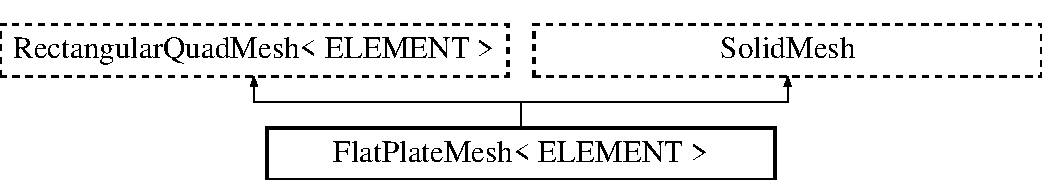
\includegraphics[height=2.000000cm]{classFlatPlateMesh}
\end{center}
\end{figure}
\subsection*{Public Member Functions}
\begin{DoxyCompactItemize}
\item 
\hyperlink{classFlatPlateMesh_a765cfa3692d1ab97790daf68d057a105}{Flat\+Plate\+Mesh} (const unsigned \&nx, const unsigned \&ny, const double \&lx, const double \&ly, Time\+Stepper $\ast$time\+\_\+stepper\+\_\+pt=\&Mesh\+::\+Default\+\_\+\+Time\+Stepper)
\begin{DoxyCompactList}\small\item\em Constructor for the mesh. \end{DoxyCompactList}\item 
void \hyperlink{classFlatPlateMesh_ad1c2d7972207aa87f17409d5d62e82fc}{assign\+\_\+undeformed\+\_\+positions} (Geom\+Object $\ast$const \&undeformed\+\_\+midplane\+\_\+pt)
\begin{DoxyCompactList}\small\item\em In all elastic problems, the nodes must be assigned an undeformed, or reference, position, corresponding to the stress-\/free state of the elastic body. This function assigns the undeformed position for the nodes on the flat plate. \end{DoxyCompactList}\end{DoxyCompactItemize}


\subsection{Detailed Description}
\subsubsection*{template$<$class E\+L\+E\+M\+E\+NT$>$\newline
class Flat\+Plate\+Mesh$<$ E\+L\+E\+M\+E\+N\+T $>$}

A 2D solid mesh for (topologically) flat 2D plates. The plate is represented by two Lagrangian coordinates that correspond to x and y in the undeformed position. The required mesh is therefore a 2D mesh and is therefore inherited from the generic Rectangular\+Quad\+Mesh 

Definition at line 146 of file plate.\+cc.



\subsection{Constructor \& Destructor Documentation}
\mbox{\Hypertarget{classFlatPlateMesh_a765cfa3692d1ab97790daf68d057a105}\label{classFlatPlateMesh_a765cfa3692d1ab97790daf68d057a105}} 
\index{Flat\+Plate\+Mesh@{Flat\+Plate\+Mesh}!Flat\+Plate\+Mesh@{Flat\+Plate\+Mesh}}
\index{Flat\+Plate\+Mesh@{Flat\+Plate\+Mesh}!Flat\+Plate\+Mesh@{Flat\+Plate\+Mesh}}
\subsubsection{\texorpdfstring{Flat\+Plate\+Mesh()}{FlatPlateMesh()}}
{\footnotesize\ttfamily template$<$class E\+L\+E\+M\+E\+NT $>$ \\
\hyperlink{classFlatPlateMesh}{Flat\+Plate\+Mesh}$<$ E\+L\+E\+M\+E\+NT $>$\+::\hyperlink{classFlatPlateMesh}{Flat\+Plate\+Mesh} (\begin{DoxyParamCaption}\item[{const unsigned \&}]{nx,  }\item[{const unsigned \&}]{ny,  }\item[{const double \&}]{lx,  }\item[{const double \&}]{ly,  }\item[{Time\+Stepper $\ast$}]{time\+\_\+stepper\+\_\+pt = {\ttfamily \&Mesh\+:\+:Default\+\_\+TimeStepper} }\end{DoxyParamCaption})}



Constructor for the mesh. 

Mesh constructor Argument list\+: nx \+: number of elements in the axial direction ny \+: number of elements in the azimuthal direction lx \+: length in the x direction ly \+: length in the y direction 

Definition at line 177 of file plate.\+cc.



\subsection{Member Function Documentation}
\mbox{\Hypertarget{classFlatPlateMesh_ad1c2d7972207aa87f17409d5d62e82fc}\label{classFlatPlateMesh_ad1c2d7972207aa87f17409d5d62e82fc}} 
\index{Flat\+Plate\+Mesh@{Flat\+Plate\+Mesh}!assign\+\_\+undeformed\+\_\+positions@{assign\+\_\+undeformed\+\_\+positions}}
\index{assign\+\_\+undeformed\+\_\+positions@{assign\+\_\+undeformed\+\_\+positions}!Flat\+Plate\+Mesh@{Flat\+Plate\+Mesh}}
\subsubsection{\texorpdfstring{assign\+\_\+undeformed\+\_\+positions()}{assign\_undeformed\_positions()}}
{\footnotesize\ttfamily template$<$class E\+L\+E\+M\+E\+NT $>$ \\
void \hyperlink{classFlatPlateMesh}{Flat\+Plate\+Mesh}$<$ E\+L\+E\+M\+E\+NT $>$\+::assign\+\_\+undeformed\+\_\+positions (\begin{DoxyParamCaption}\item[{Geom\+Object $\ast$const \&}]{undeformed\+\_\+midplane\+\_\+pt }\end{DoxyParamCaption})}



In all elastic problems, the nodes must be assigned an undeformed, or reference, position, corresponding to the stress-\/free state of the elastic body. This function assigns the undeformed position for the nodes on the flat plate. 

Set the undeformed coordinates of the nodes. 

Definition at line 224 of file plate.\+cc.



Referenced by Plate\+Problem$<$ E\+L\+E\+M\+E\+N\+T $>$\+::\+Plate\+Problem().



The documentation for this class was generated from the following file\+:\begin{DoxyCompactItemize}
\item 
\hyperlink{plate_8cc}{plate.\+cc}\end{DoxyCompactItemize}

\hypertarget{classMyLinearisedShellProblem}{}\section{My\+Linearised\+Shell\+Problem$<$ E\+L\+E\+M\+E\+NT, D\+IM, N\+N\+O\+D\+E\+\_\+1D $>$ Class Template Reference}
\label{classMyLinearisedShellProblem}\index{My\+Linearised\+Shell\+Problem$<$ E\+L\+E\+M\+E\+N\+T, D\+I\+M, N\+N\+O\+D\+E\+\_\+1\+D $>$@{My\+Linearised\+Shell\+Problem$<$ E\+L\+E\+M\+E\+N\+T, D\+I\+M, N\+N\+O\+D\+E\+\_\+1\+D $>$}}


2D linearised shell problem.  


Inheritance diagram for My\+Linearised\+Shell\+Problem$<$ E\+L\+E\+M\+E\+NT, D\+IM, N\+N\+O\+D\+E\+\_\+1D $>$\+:\begin{figure}[H]
\begin{center}
\leavevmode
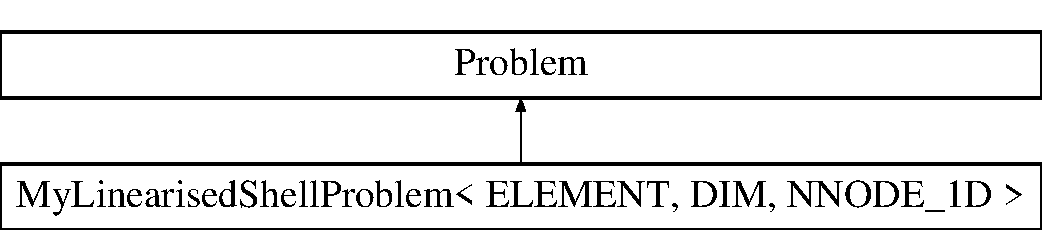
\includegraphics[height=2.000000cm]{classMyLinearisedShellProblem}
\end{center}
\end{figure}
\subsection*{Public Member Functions}
\begin{DoxyCompactItemize}
\item 
\hyperlink{classMyLinearisedShellProblem_a2ccc4ed3e631ca68d1d86423ef8eeb03}{My\+Linearised\+Shell\+Problem} (typename \hyperlink{classoomph_1_1MyShellEquations}{My\+Shell\+Equations}$<$ D\+IM, N\+N\+O\+D\+E\+\_\+1D $>$\+::Source\+Fct\+Pt source\+\_\+fct\+\_\+pt, const string \&node\+\_\+file\+\_\+name, const string \&element\+\_\+file\+\_\+name, const string \&poly\+\_\+file\+\_\+name)
\begin{DoxyCompactList}\small\item\em Constructor\+: Pass number of elements and pointer to source function. \end{DoxyCompactList}\item 
\hyperlink{classMyLinearisedShellProblem_a8720e7226adb9f23266fe729f7e4eb5a}{$\sim$\+My\+Linearised\+Shell\+Problem} ()
\begin{DoxyCompactList}\small\item\em Destructor (empty) \end{DoxyCompactList}\item 
void \hyperlink{classMyLinearisedShellProblem_a81d050ee6958694b7645ea73cc8e4e9f}{actions\+\_\+before\+\_\+newton\+\_\+solve} ()
\begin{DoxyCompactList}\small\item\em Update the problem specs before solve\+: (Re)set boundary conditions. \end{DoxyCompactList}\item 
void \hyperlink{classMyLinearisedShellProblem_a8ad6606f22859a5bd32d238bcc10efd1}{actions\+\_\+after\+\_\+newton\+\_\+solve} ()
\begin{DoxyCompactList}\small\item\em Update the problem specs after solve (empty) \end{DoxyCompactList}\item 
void \hyperlink{classMyLinearisedShellProblem_a5894d8fae239fd5255b6a661cbc23fa5}{doc\+\_\+solution} (Doc\+Info \&doc\+\_\+info)
\begin{DoxyCompactList}\small\item\em Doc the solution, pass the number of the case considered, so that output files can be distinguished. \end{DoxyCompactList}\item 
void \hyperlink{classMyLinearisedShellProblem_ab9255e3cbaae69ad5d61757d891b633e}{parameter\+\_\+study} ()
\begin{DoxyCompactList}\small\item\em Solver loop to perform parameter study. \end{DoxyCompactList}\end{DoxyCompactItemize}
\subsection*{Private Attributes}
\begin{DoxyCompactItemize}
\item 
\hyperlink{classoomph_1_1MyShellEquations}{My\+Shell\+Equations}$<$ D\+IM, N\+N\+O\+D\+E\+\_\+1D $>$\+::Source\+Fct\+Pt \hyperlink{classMyLinearisedShellProblem_a55fd5e4ce59d478cb41bd8457e868dea}{Source\+\_\+fct\+\_\+pt}
\begin{DoxyCompactList}\small\item\em Pointer to source function. \end{DoxyCompactList}\item 
Geom\+Object $\ast$ \hyperlink{classMyLinearisedShellProblem_a18e84aab4a7fad179e35d381e61c4584}{Undef\+\_\+midplane\+\_\+pt}
\begin{DoxyCompactList}\small\item\em Pointer to geometric object that represents the shell\textquotesingle{}s undeformed shape. \end{DoxyCompactList}\end{DoxyCompactItemize}


\subsection{Detailed Description}
\subsubsection*{template$<$class E\+L\+E\+M\+E\+NT, unsigned D\+IM, unsigned N\+N\+O\+D\+E\+\_\+1D$>$\newline
class My\+Linearised\+Shell\+Problem$<$ E\+L\+E\+M\+E\+N\+T, D\+I\+M, N\+N\+O\+D\+E\+\_\+1\+D $>$}

2D linearised shell problem. 

Definition at line 1526 of file unstructured\+\_\+clamped\+\_\+curved\+\_\+shell.\+cc.



\subsection{Constructor \& Destructor Documentation}
\mbox{\Hypertarget{classMyLinearisedShellProblem_a2ccc4ed3e631ca68d1d86423ef8eeb03}\label{classMyLinearisedShellProblem_a2ccc4ed3e631ca68d1d86423ef8eeb03}} 
\index{My\+Linearised\+Shell\+Problem@{My\+Linearised\+Shell\+Problem}!My\+Linearised\+Shell\+Problem@{My\+Linearised\+Shell\+Problem}}
\index{My\+Linearised\+Shell\+Problem@{My\+Linearised\+Shell\+Problem}!My\+Linearised\+Shell\+Problem@{My\+Linearised\+Shell\+Problem}}
\subsubsection{\texorpdfstring{My\+Linearised\+Shell\+Problem()}{MyLinearisedShellProblem()}}
{\footnotesize\ttfamily template$<$class E\+L\+E\+M\+E\+NT , unsigned D\+IM, unsigned N\+N\+O\+D\+E\+\_\+1D$>$ \\
\hyperlink{classMyLinearisedShellProblem}{My\+Linearised\+Shell\+Problem}$<$ E\+L\+E\+M\+E\+NT, D\+IM, N\+N\+O\+D\+E\+\_\+1D $>$\+::\hyperlink{classMyLinearisedShellProblem}{My\+Linearised\+Shell\+Problem} (\begin{DoxyParamCaption}\item[{typename \hyperlink{classoomph_1_1MyShellEquations}{My\+Shell\+Equations}$<$ D\+IM, N\+N\+O\+D\+E\+\_\+1D $>$\+::Source\+Fct\+Pt}]{source\+\_\+fct\+\_\+pt,  }\item[{const string \&}]{node\+\_\+file\+\_\+name,  }\item[{const string \&}]{element\+\_\+file\+\_\+name,  }\item[{const string \&}]{poly\+\_\+file\+\_\+name }\end{DoxyParamCaption})}



Constructor\+: Pass number of elements and pointer to source function. 

Constructor for 2D Shell problem. Discretise the 2D domain with n\+\_\+element elements of type E\+L\+E\+M\+E\+NT. Specify function pointer to source function. loop over the nodes on the boundary 

Definition at line 1571 of file unstructured\+\_\+clamped\+\_\+curved\+\_\+shell.\+cc.

\mbox{\Hypertarget{classMyLinearisedShellProblem_a8720e7226adb9f23266fe729f7e4eb5a}\label{classMyLinearisedShellProblem_a8720e7226adb9f23266fe729f7e4eb5a}} 
\index{My\+Linearised\+Shell\+Problem@{My\+Linearised\+Shell\+Problem}!````~My\+Linearised\+Shell\+Problem@{$\sim$\+My\+Linearised\+Shell\+Problem}}
\index{````~My\+Linearised\+Shell\+Problem@{$\sim$\+My\+Linearised\+Shell\+Problem}!My\+Linearised\+Shell\+Problem@{My\+Linearised\+Shell\+Problem}}
\subsubsection{\texorpdfstring{$\sim$\+My\+Linearised\+Shell\+Problem()}{~MyLinearisedShellProblem()}}
{\footnotesize\ttfamily template$<$class E\+L\+E\+M\+E\+NT, unsigned D\+IM, unsigned N\+N\+O\+D\+E\+\_\+1D$>$ \\
\hyperlink{classMyLinearisedShellProblem}{My\+Linearised\+Shell\+Problem}$<$ E\+L\+E\+M\+E\+NT, D\+IM, N\+N\+O\+D\+E\+\_\+1D $>$\+::$\sim$\hyperlink{classMyLinearisedShellProblem}{My\+Linearised\+Shell\+Problem} (\begin{DoxyParamCaption}{ }\end{DoxyParamCaption})\hspace{0.3cm}{\ttfamily [inline]}}



Destructor (empty) 



Definition at line 1538 of file unstructured\+\_\+clamped\+\_\+curved\+\_\+shell.\+cc.



\subsection{Member Function Documentation}
\mbox{\Hypertarget{classMyLinearisedShellProblem_a8ad6606f22859a5bd32d238bcc10efd1}\label{classMyLinearisedShellProblem_a8ad6606f22859a5bd32d238bcc10efd1}} 
\index{My\+Linearised\+Shell\+Problem@{My\+Linearised\+Shell\+Problem}!actions\+\_\+after\+\_\+newton\+\_\+solve@{actions\+\_\+after\+\_\+newton\+\_\+solve}}
\index{actions\+\_\+after\+\_\+newton\+\_\+solve@{actions\+\_\+after\+\_\+newton\+\_\+solve}!My\+Linearised\+Shell\+Problem@{My\+Linearised\+Shell\+Problem}}
\subsubsection{\texorpdfstring{actions\+\_\+after\+\_\+newton\+\_\+solve()}{actions\_after\_newton\_solve()}}
{\footnotesize\ttfamily template$<$class E\+L\+E\+M\+E\+NT, unsigned D\+IM, unsigned N\+N\+O\+D\+E\+\_\+1D$>$ \\
void \hyperlink{classMyLinearisedShellProblem}{My\+Linearised\+Shell\+Problem}$<$ E\+L\+E\+M\+E\+NT, D\+IM, N\+N\+O\+D\+E\+\_\+1D $>$\+::actions\+\_\+after\+\_\+newton\+\_\+solve (\begin{DoxyParamCaption}{ }\end{DoxyParamCaption})\hspace{0.3cm}{\ttfamily [inline]}}



Update the problem specs after solve (empty) 



Definition at line 1547 of file unstructured\+\_\+clamped\+\_\+curved\+\_\+shell.\+cc.

\mbox{\Hypertarget{classMyLinearisedShellProblem_a81d050ee6958694b7645ea73cc8e4e9f}\label{classMyLinearisedShellProblem_a81d050ee6958694b7645ea73cc8e4e9f}} 
\index{My\+Linearised\+Shell\+Problem@{My\+Linearised\+Shell\+Problem}!actions\+\_\+before\+\_\+newton\+\_\+solve@{actions\+\_\+before\+\_\+newton\+\_\+solve}}
\index{actions\+\_\+before\+\_\+newton\+\_\+solve@{actions\+\_\+before\+\_\+newton\+\_\+solve}!My\+Linearised\+Shell\+Problem@{My\+Linearised\+Shell\+Problem}}
\subsubsection{\texorpdfstring{actions\+\_\+before\+\_\+newton\+\_\+solve()}{actions\_before\_newton\_solve()}}
{\footnotesize\ttfamily template$<$class E\+L\+E\+M\+E\+NT , unsigned D\+IM, unsigned N\+N\+O\+D\+E\+\_\+1D$>$ \\
void \hyperlink{classMyLinearisedShellProblem}{My\+Linearised\+Shell\+Problem}$<$ E\+L\+E\+M\+E\+NT, D\+IM, N\+N\+O\+D\+E\+\_\+1D $>$\+::actions\+\_\+before\+\_\+newton\+\_\+solve (\begin{DoxyParamCaption}{ }\end{DoxyParamCaption})}



Update the problem specs before solve\+: (Re)set boundary conditions. 

Update the problem specs before solve\+: (Re)set boundary values from the exact solution. loop over the nodes on the boundary 

Definition at line 1700 of file unstructured\+\_\+clamped\+\_\+curved\+\_\+shell.\+cc.



References Physical\+\_\+\+Variables\+::get\+\_\+exact\+\_\+u().

\mbox{\Hypertarget{classMyLinearisedShellProblem_a5894d8fae239fd5255b6a661cbc23fa5}\label{classMyLinearisedShellProblem_a5894d8fae239fd5255b6a661cbc23fa5}} 
\index{My\+Linearised\+Shell\+Problem@{My\+Linearised\+Shell\+Problem}!doc\+\_\+solution@{doc\+\_\+solution}}
\index{doc\+\_\+solution@{doc\+\_\+solution}!My\+Linearised\+Shell\+Problem@{My\+Linearised\+Shell\+Problem}}
\subsubsection{\texorpdfstring{doc\+\_\+solution()}{doc\_solution()}}
{\footnotesize\ttfamily template$<$class E\+L\+E\+M\+E\+NT , unsigned D\+IM, unsigned N\+N\+O\+D\+E\+\_\+1D$>$ \\
void \hyperlink{classMyLinearisedShellProblem}{My\+Linearised\+Shell\+Problem}$<$ E\+L\+E\+M\+E\+NT, D\+IM, N\+N\+O\+D\+E\+\_\+1D $>$\+::doc\+\_\+solution (\begin{DoxyParamCaption}\item[{Doc\+Info \&}]{doc\+\_\+info }\end{DoxyParamCaption})}



Doc the solution, pass the number of the case considered, so that output files can be distinguished. 

Doc the solution in tecplot format. Label files with label. 

Definition at line 1740 of file unstructured\+\_\+clamped\+\_\+curved\+\_\+shell.\+cc.

\mbox{\Hypertarget{classMyLinearisedShellProblem_ab9255e3cbaae69ad5d61757d891b633e}\label{classMyLinearisedShellProblem_ab9255e3cbaae69ad5d61757d891b633e}} 
\index{My\+Linearised\+Shell\+Problem@{My\+Linearised\+Shell\+Problem}!parameter\+\_\+study@{parameter\+\_\+study}}
\index{parameter\+\_\+study@{parameter\+\_\+study}!My\+Linearised\+Shell\+Problem@{My\+Linearised\+Shell\+Problem}}
\subsubsection{\texorpdfstring{parameter\+\_\+study()}{parameter\_study()}}
{\footnotesize\ttfamily template$<$class E\+L\+E\+M\+E\+NT , unsigned D\+IM, unsigned N\+N\+O\+D\+E\+\_\+1D$>$ \\
void \hyperlink{classMyLinearisedShellProblem}{My\+Linearised\+Shell\+Problem}$<$ E\+L\+E\+M\+E\+NT, D\+IM, N\+N\+O\+D\+E\+\_\+1D $>$\+::parameter\+\_\+study (\begin{DoxyParamCaption}{ }\end{DoxyParamCaption})}



Solver loop to perform parameter study. 



Definition at line 1764 of file unstructured\+\_\+clamped\+\_\+curved\+\_\+shell.\+cc.



References Physical\+\_\+\+Variables\+::\+P\+\_\+ext.



Referenced by main().



\subsection{Member Data Documentation}
\mbox{\Hypertarget{classMyLinearisedShellProblem_a55fd5e4ce59d478cb41bd8457e868dea}\label{classMyLinearisedShellProblem_a55fd5e4ce59d478cb41bd8457e868dea}} 
\index{My\+Linearised\+Shell\+Problem@{My\+Linearised\+Shell\+Problem}!Source\+\_\+fct\+\_\+pt@{Source\+\_\+fct\+\_\+pt}}
\index{Source\+\_\+fct\+\_\+pt@{Source\+\_\+fct\+\_\+pt}!My\+Linearised\+Shell\+Problem@{My\+Linearised\+Shell\+Problem}}
\subsubsection{\texorpdfstring{Source\+\_\+fct\+\_\+pt}{Source\_fct\_pt}}
{\footnotesize\ttfamily template$<$class E\+L\+E\+M\+E\+NT, unsigned D\+IM, unsigned N\+N\+O\+D\+E\+\_\+1D$>$ \\
\hyperlink{classoomph_1_1MyShellEquations}{My\+Shell\+Equations}$<$D\+IM,N\+N\+O\+D\+E\+\_\+1D$>$\+::Source\+Fct\+Pt \hyperlink{classMyLinearisedShellProblem}{My\+Linearised\+Shell\+Problem}$<$ E\+L\+E\+M\+E\+NT, D\+IM, N\+N\+O\+D\+E\+\_\+1D $>$\+::Source\+\_\+fct\+\_\+pt\hspace{0.3cm}{\ttfamily [private]}}



Pointer to source function. 



Definition at line 1558 of file unstructured\+\_\+clamped\+\_\+curved\+\_\+shell.\+cc.

\mbox{\Hypertarget{classMyLinearisedShellProblem_a18e84aab4a7fad179e35d381e61c4584}\label{classMyLinearisedShellProblem_a18e84aab4a7fad179e35d381e61c4584}} 
\index{My\+Linearised\+Shell\+Problem@{My\+Linearised\+Shell\+Problem}!Undef\+\_\+midplane\+\_\+pt@{Undef\+\_\+midplane\+\_\+pt}}
\index{Undef\+\_\+midplane\+\_\+pt@{Undef\+\_\+midplane\+\_\+pt}!My\+Linearised\+Shell\+Problem@{My\+Linearised\+Shell\+Problem}}
\subsubsection{\texorpdfstring{Undef\+\_\+midplane\+\_\+pt}{Undef\_midplane\_pt}}
{\footnotesize\ttfamily template$<$class E\+L\+E\+M\+E\+NT, unsigned D\+IM, unsigned N\+N\+O\+D\+E\+\_\+1D$>$ \\
Geom\+Object$\ast$ \hyperlink{classMyLinearisedShellProblem}{My\+Linearised\+Shell\+Problem}$<$ E\+L\+E\+M\+E\+NT, D\+IM, N\+N\+O\+D\+E\+\_\+1D $>$\+::Undef\+\_\+midplane\+\_\+pt\hspace{0.3cm}{\ttfamily [private]}}



Pointer to geometric object that represents the shell\textquotesingle{}s undeformed shape. 



Definition at line 1560 of file unstructured\+\_\+clamped\+\_\+curved\+\_\+shell.\+cc.



The documentation for this class was generated from the following file\+:\begin{DoxyCompactItemize}
\item 
\hyperlink{unstructured__clamped__curved__shell_8cc}{unstructured\+\_\+clamped\+\_\+curved\+\_\+shell.\+cc}\end{DoxyCompactItemize}

\hypertarget{classoomph_1_1MyShellEquations}{}\section{oomph\+:\+:My\+Shell\+Equations$<$ D\+IM, N\+N\+O\+D\+E\+\_\+1D $>$ Class Template Reference}
\label{classoomph_1_1MyShellEquations}\index{oomph\+::\+My\+Shell\+Equations$<$ D\+I\+M, N\+N\+O\+D\+E\+\_\+1\+D $>$@{oomph\+::\+My\+Shell\+Equations$<$ D\+I\+M, N\+N\+O\+D\+E\+\_\+1\+D $>$}}
Inheritance diagram for oomph\+:\+:My\+Shell\+Equations$<$ D\+IM, N\+N\+O\+D\+E\+\_\+1D $>$\+:\begin{figure}[H]
\begin{center}
\leavevmode
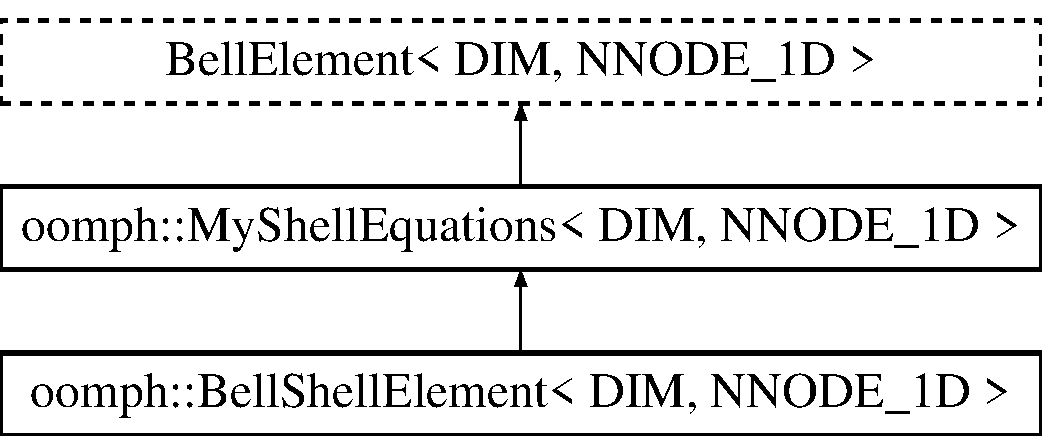
\includegraphics[height=3.000000cm]{classoomph_1_1MyShellEquations}
\end{center}
\end{figure}
\subsection*{Public Types}
\begin{DoxyCompactItemize}
\item 
typedef void($\ast$ \hyperlink{classoomph_1_1MyShellEquations_a056d2488b6e65787f5c9935a321b7a9b}{Source\+Fct\+Pt}) (const Vector$<$ double $>$ \&x, const Vector$<$ double $>$ \&unit\+\_\+n, Vector$<$ double $>$ \&f)
\begin{DoxyCompactList}\small\item\em Function pointer to source function fct(x,f(x)) -- x is a Vector! \end{DoxyCompactList}\item 
typedef void($\ast$ \hyperlink{classoomph_1_1MyShellEquations_a954dcc1b78710f331ed390b716aa07dd}{Source\+Fct\+Gradient\+Pt}) (const Vector$<$ double $>$ \&x, Vector$<$ double $>$ \&gradient)
\begin{DoxyCompactList}\small\item\em Function pointer to gradient of source function fct(x,g(x)) -- x is a Vector! \end{DoxyCompactList}\end{DoxyCompactItemize}
\subsection*{Public Member Functions}
\begin{DoxyCompactItemize}
\item 
\hyperlink{classoomph_1_1MyShellEquations_a4d459716fb0b2b66ece7d87c0feac9ed}{My\+Shell\+Equations} ()
\begin{DoxyCompactList}\small\item\em Constructor (must initialise the Source\+\_\+fct\+\_\+pt to null) \end{DoxyCompactList}\item 
\hyperlink{classoomph_1_1MyShellEquations_af92d9d503350b3c84d309b1e70911e27}{My\+Shell\+Equations} (const \hyperlink{classoomph_1_1MyShellEquations}{My\+Shell\+Equations} \&dummy)
\begin{DoxyCompactList}\small\item\em Broken copy constructor. \end{DoxyCompactList}\item 
virtual unsigned \hyperlink{classoomph_1_1MyShellEquations_a983c9be2c162eccec2f41c391722f0aa}{u\+\_\+index\+\_\+shell} () const
\begin{DoxyCompactList}\small\item\em Return the index at which the unknown value is stored. In derived multi-\/physics elements, this function should be overloaded to reflect the chosen storage scheme. Note that these equations require that the unknown is always stored at the same index at each node. \end{DoxyCompactList}\item 
void \hyperlink{classoomph_1_1MyShellEquations_aa5434267aa4c3a6f0b86d9afbb18f0a5}{output} (std\+::ostream \&outfile)
\begin{DoxyCompactList}\small\item\em Output with default number of plot points. \end{DoxyCompactList}\item 
void \hyperlink{classoomph_1_1MyShellEquations_ad4ad93d1ef0640f5ded693e0bc46aeb6}{output} (std\+::ostream \&outfile, const unsigned \&n\+\_\+plot)
\begin{DoxyCompactList}\small\item\em Output FE representation of soln\+: x,y,u or x,y,z,u at n\+\_\+plot$^\wedge$\+D\+IM plot points. \end{DoxyCompactList}\item 
void \hyperlink{classoomph_1_1MyShellEquations_aa8411334811e9b382d2c96051ac4b2ba}{output} (F\+I\+LE $\ast$file\+\_\+pt)
\begin{DoxyCompactList}\small\item\em C\+\_\+style output with default number of plot points. \end{DoxyCompactList}\item 
void \hyperlink{classoomph_1_1MyShellEquations_adc1fcb6052b2cd07efe4d7d841ed6723}{output} (F\+I\+LE $\ast$file\+\_\+pt, const unsigned \&n\+\_\+plot)
\begin{DoxyCompactList}\small\item\em C-\/style output FE representation of soln\+: x,y,u or x,y,z,u at n\+\_\+plot$^\wedge$\+D\+IM plot points. \end{DoxyCompactList}\item 
void \hyperlink{classoomph_1_1MyShellEquations_a882f6447d8e204962a3f2a350c6315c4}{output\+\_\+fct} (std\+::ostream \&outfile, const unsigned \&n\+\_\+plot, Finite\+Element\+::\+Steady\+Exact\+Solution\+Fct\+Pt exact\+\_\+soln\+\_\+pt)
\begin{DoxyCompactList}\small\item\em Output exact soln\+: x,y,u\+\_\+exact or x,y,z,u\+\_\+exact at n\+\_\+plot$^\wedge$\+D\+IM plot points. \end{DoxyCompactList}\item 
virtual void \hyperlink{classoomph_1_1MyShellEquations_a7022e91eaf4bff9044e46549bbe0c3f5}{output\+\_\+fct} (std\+::ostream \&outfile, const unsigned \&n\+\_\+plot, const double \&time, Finite\+Element\+::\+Unsteady\+Exact\+Solution\+Fct\+Pt exact\+\_\+soln\+\_\+pt)
\begin{DoxyCompactList}\small\item\em Output exact soln\+: x,y,u\+\_\+exact or x,y,z,u\+\_\+exact at n\+\_\+plot$^\wedge$\+D\+IM plot points (dummy time-\/dependent version to keep intel compiler happy) \end{DoxyCompactList}\item 
void \hyperlink{classoomph_1_1MyShellEquations_a72cb38c977990a46780dfedab0fee8b8}{compute\+\_\+error} (std\+::ostream \&outfile, Finite\+Element\+::\+Steady\+Exact\+Solution\+Fct\+Pt exact\+\_\+soln\+\_\+pt, double \&error, double \&norm)
\begin{DoxyCompactList}\small\item\em Get error against and norm of exact solution. \end{DoxyCompactList}\item 
void \hyperlink{classoomph_1_1MyShellEquations_a6a62a37fa44a5001c167071f9bf80c2f}{compute\+\_\+error} (std\+::ostream \&outfile, Finite\+Element\+::\+Unsteady\+Exact\+Solution\+Fct\+Pt exact\+\_\+soln\+\_\+pt, const double \&time, double \&error, double \&norm)
\begin{DoxyCompactList}\small\item\em Dummy, time dependent error checker. \end{DoxyCompactList}\item 
\hyperlink{classoomph_1_1MyShellEquations_a056d2488b6e65787f5c9935a321b7a9b}{Source\+Fct\+Pt} \& \hyperlink{classoomph_1_1MyShellEquations_a8aee1d7092584b9ad7095dfd905f5893}{source\+\_\+fct\+\_\+pt} ()
\begin{DoxyCompactList}\small\item\em Access function\+: Pointer to source function. \end{DoxyCompactList}\item 
\hyperlink{classoomph_1_1MyShellEquations_a056d2488b6e65787f5c9935a321b7a9b}{Source\+Fct\+Pt} \hyperlink{classoomph_1_1MyShellEquations_a3cf0287a7fcc34f88c011805ae18fdcb}{source\+\_\+fct\+\_\+pt} () const
\begin{DoxyCompactList}\small\item\em Access function\+: Pointer to source function. Const version. \end{DoxyCompactList}\item 
\hyperlink{classoomph_1_1MyShellEquations_a954dcc1b78710f331ed390b716aa07dd}{Source\+Fct\+Gradient\+Pt} \& \hyperlink{classoomph_1_1MyShellEquations_a1ade98830b556492e11aef07cf34d3ed}{source\+\_\+fct\+\_\+gradient\+\_\+pt} ()
\begin{DoxyCompactList}\small\item\em Access function\+: Pointer to gradient of source function. \end{DoxyCompactList}\item 
\hyperlink{classoomph_1_1MyShellEquations_a954dcc1b78710f331ed390b716aa07dd}{Source\+Fct\+Gradient\+Pt} \hyperlink{classoomph_1_1MyShellEquations_aeb57d576c45c382206c6af6b8b06b575}{source\+\_\+fct\+\_\+gradient\+\_\+pt} () const
\begin{DoxyCompactList}\small\item\em Access function\+: Pointer to gradient source function. Const version. \end{DoxyCompactList}\item 
Geom\+Object $\ast$\& \hyperlink{classoomph_1_1MyShellEquations_acf40f3e2413d4640be3ba3664b8d0426}{undeformed\+\_\+midplane\+\_\+pt} ()
\begin{DoxyCompactList}\small\item\em Access function\+: Undeformed shell. \end{DoxyCompactList}\item 
virtual void \hyperlink{classoomph_1_1MyShellEquations_a6c1858131a4ddd0c59a45449db7e182a}{get\+\_\+source\+\_\+function} (const unsigned \&ipt, const Vector$<$ double $>$ \&x, const Vector$<$ double $>$ \&unit\+\_\+n, Vector$<$ double $>$ \&source) const
\item 
void \hyperlink{classoomph_1_1MyShellEquations_ac612ccae94aed8f8ce5b9cc9410f5424}{fill\+\_\+in\+\_\+contribution\+\_\+to\+\_\+residuals} (Vector$<$ double $>$ \&residuals)
\begin{DoxyCompactList}\small\item\em Add the element\textquotesingle{}s contribution to its residual vector (wrapper) \end{DoxyCompactList}\item 
Vector$<$ double $>$ \hyperlink{classoomph_1_1MyShellEquations_a6f170026c39f99db20110a6d6e76e6c0}{interpolated\+\_\+u\+\_\+shell} (const Vector$<$ double $>$ \&s) const
\begin{DoxyCompactList}\small\item\em Return FE representation of unknown value u(s) at local coordinate s. \end{DoxyCompactList}\item 
unsigned \hyperlink{classoomph_1_1MyShellEquations_ab78a1d617fdd782b3e60ffd89e0c4737}{self\+\_\+test} ()
\begin{DoxyCompactList}\small\item\em Self-\/test\+: Return 0 for OK. \end{DoxyCompactList}\end{DoxyCompactItemize}
\subsection*{Protected Member Functions}
\begin{DoxyCompactItemize}
\item 
virtual double \hyperlink{classoomph_1_1MyShellEquations_ae5efd29cb214218d41d29abab4dcec51}{d2shape\+\_\+and\+\_\+d2test\+\_\+eulerian\+\_\+shell} (const Vector$<$ double $>$ \&s, Shape \&psi, D\+Shape \&dpsidx, D\+Shape \&d2psidx, Shape \&test, D\+Shape \&dtestdx, D\+Shape \&d2testdx) const =0
\begin{DoxyCompactList}\small\item\em Shape/test functions and derivs w.\+r.\+t. to global coords at local coord. s; return Jacobian of mapping. \end{DoxyCompactList}\item 
virtual double \hyperlink{classoomph_1_1MyShellEquations_ac0cb5a90f9eceb2406c21c1e1dc662e7}{dshape\+\_\+and\+\_\+dtest\+\_\+eulerian\+\_\+shell} (const Vector$<$ double $>$ \&s, Shape \&psi, D\+Shape \&dpsidx, Shape \&test, D\+Shape \&dtestdx) const =0
\item 
virtual double \hyperlink{classoomph_1_1MyShellEquations_af8f15f0d678c85535bbc3390399dafdd}{d2shape\+\_\+and\+\_\+d2test\+\_\+eulerian\+\_\+at\+\_\+knot\+\_\+shell} (const unsigned \&ipt, Shape \&psi, D\+Shape \&dpsidx, D\+Shape \&d2psidx, Shape \&test, D\+Shape \&dtestdx, D\+Shape \&d2testdx) const =0
\begin{DoxyCompactList}\small\item\em Shape/test functions and derivs w.\+r.\+t. to global coords at integration point ipt; return Jacobian of mapping. \end{DoxyCompactList}\item 
virtual double \hyperlink{classoomph_1_1MyShellEquations_a0800ff2f9716a3b0327624948ce792e1}{dshape\+\_\+and\+\_\+dtest\+\_\+eulerian\+\_\+at\+\_\+knot\+\_\+shell} (const unsigned \&ipt, Shape \&psi, D\+Shape \&dpsidx, Shape \&test, D\+Shape \&dtestdx) const =0
\item 
virtual void \hyperlink{classoomph_1_1MyShellEquations_a39b639b46ce1b2fcd53465b02da47f78}{fill\+\_\+in\+\_\+generic\+\_\+residual\+\_\+contribution\+\_\+shell} (Vector$<$ double $>$ \&residuals, Dense\+Matrix$<$ double $>$ \&jacobian, const unsigned \&flag)
\begin{DoxyCompactList}\small\item\em Compute element residual Vector only (if flag=and/or element Jacobian matrix. \end{DoxyCompactList}\end{DoxyCompactItemize}
\subsection*{Protected Attributes}
\begin{DoxyCompactItemize}
\item 
\hyperlink{classoomph_1_1MyShellEquations_a056d2488b6e65787f5c9935a321b7a9b}{Source\+Fct\+Pt} \hyperlink{classoomph_1_1MyShellEquations_a60988a3591e836a2afecf416d1287985}{Source\+\_\+fct\+\_\+pt}
\begin{DoxyCompactList}\small\item\em Pointer to source function\+: \end{DoxyCompactList}\item 
\hyperlink{classoomph_1_1MyShellEquations_a954dcc1b78710f331ed390b716aa07dd}{Source\+Fct\+Gradient\+Pt} \hyperlink{classoomph_1_1MyShellEquations_ab45cb2cb03c75c4410fa4288f9a8be90}{Source\+\_\+fct\+\_\+gradient\+\_\+pt}
\begin{DoxyCompactList}\small\item\em Pointer to gradient of source function. \end{DoxyCompactList}\item 
Geom\+Object $\ast$ \hyperlink{classoomph_1_1MyShellEquations_acf0107874213e70145eae84dfb3d4b5a}{Undeformed\+\_\+midplane\+\_\+pt}
\begin{DoxyCompactList}\small\item\em Pointer to undeformed beam\+: \end{DoxyCompactList}\item 
double $\ast$ \hyperlink{classoomph_1_1MyShellEquations_a909b1e9608109048d446f86ca3c7d02d}{Sigma0\+\_\+pt}
\begin{DoxyCompactList}\small\item\em Pointer to axial prestress. \end{DoxyCompactList}\item 
double $\ast$ \hyperlink{classoomph_1_1MyShellEquations_a6cd7175e7205dc7cea4e0e505f3cb8b9}{H\+\_\+pt}
\begin{DoxyCompactList}\small\item\em Pointer to wall thickness. \end{DoxyCompactList}\item 
double $\ast$ \hyperlink{classoomph_1_1MyShellEquations_a6201b3eced8396c6e2246df94c946537}{Lambda\+\_\+sq\+\_\+pt}
\begin{DoxyCompactList}\small\item\em Pointer to Timescale ratio. \end{DoxyCompactList}\end{DoxyCompactItemize}


\subsection{Detailed Description}
\subsubsection*{template$<$unsigned D\+IM, unsigned N\+N\+O\+D\+E\+\_\+1D$>$\newline
class oomph\+::\+My\+Shell\+Equations$<$ D\+I\+M, N\+N\+O\+D\+E\+\_\+1\+D $>$}

A class for all subparametric elements that solve the linear shell equations. This contains the generic maths. Shape functions, geometric mapping etc. must get implemented in derived class. 

Definition at line 65 of file unstructured\+\_\+clamped\+\_\+curved\+\_\+shell.\+cc.



\subsection{Member Typedef Documentation}
\mbox{\Hypertarget{classoomph_1_1MyShellEquations_a954dcc1b78710f331ed390b716aa07dd}\label{classoomph_1_1MyShellEquations_a954dcc1b78710f331ed390b716aa07dd}} 
\index{oomph\+::\+My\+Shell\+Equations@{oomph\+::\+My\+Shell\+Equations}!Source\+Fct\+Gradient\+Pt@{Source\+Fct\+Gradient\+Pt}}
\index{Source\+Fct\+Gradient\+Pt@{Source\+Fct\+Gradient\+Pt}!oomph\+::\+My\+Shell\+Equations@{oomph\+::\+My\+Shell\+Equations}}
\subsubsection{\texorpdfstring{Source\+Fct\+Gradient\+Pt}{SourceFctGradientPt}}
{\footnotesize\ttfamily template$<$unsigned D\+IM, unsigned N\+N\+O\+D\+E\+\_\+1D$>$ \\
typedef void($\ast$ \hyperlink{classoomph_1_1MyShellEquations}{oomph\+::\+My\+Shell\+Equations}$<$ D\+IM, N\+N\+O\+D\+E\+\_\+1D $>$\+::Source\+Fct\+Gradient\+Pt) (const Vector$<$ double $>$ \&x, Vector$<$ double $>$ \&gradient)}



Function pointer to gradient of source function fct(x,g(x)) -- x is a Vector! 



Definition at line 77 of file unstructured\+\_\+clamped\+\_\+curved\+\_\+shell.\+cc.

\mbox{\Hypertarget{classoomph_1_1MyShellEquations_a056d2488b6e65787f5c9935a321b7a9b}\label{classoomph_1_1MyShellEquations_a056d2488b6e65787f5c9935a321b7a9b}} 
\index{oomph\+::\+My\+Shell\+Equations@{oomph\+::\+My\+Shell\+Equations}!Source\+Fct\+Pt@{Source\+Fct\+Pt}}
\index{Source\+Fct\+Pt@{Source\+Fct\+Pt}!oomph\+::\+My\+Shell\+Equations@{oomph\+::\+My\+Shell\+Equations}}
\subsubsection{\texorpdfstring{Source\+Fct\+Pt}{SourceFctPt}}
{\footnotesize\ttfamily template$<$unsigned D\+IM, unsigned N\+N\+O\+D\+E\+\_\+1D$>$ \\
typedef void($\ast$ \hyperlink{classoomph_1_1MyShellEquations}{oomph\+::\+My\+Shell\+Equations}$<$ D\+IM, N\+N\+O\+D\+E\+\_\+1D $>$\+::Source\+Fct\+Pt) (const Vector$<$ double $>$ \&x, const Vector$<$ double $>$ \&unit\+\_\+n, Vector$<$ double $>$ \&f)}



Function pointer to source function fct(x,f(x)) -- x is a Vector! 



Definition at line 72 of file unstructured\+\_\+clamped\+\_\+curved\+\_\+shell.\+cc.



\subsection{Constructor \& Destructor Documentation}
\mbox{\Hypertarget{classoomph_1_1MyShellEquations_a4d459716fb0b2b66ece7d87c0feac9ed}\label{classoomph_1_1MyShellEquations_a4d459716fb0b2b66ece7d87c0feac9ed}} 
\index{oomph\+::\+My\+Shell\+Equations@{oomph\+::\+My\+Shell\+Equations}!My\+Shell\+Equations@{My\+Shell\+Equations}}
\index{My\+Shell\+Equations@{My\+Shell\+Equations}!oomph\+::\+My\+Shell\+Equations@{oomph\+::\+My\+Shell\+Equations}}
\subsubsection{\texorpdfstring{My\+Shell\+Equations()}{MyShellEquations()}\hspace{0.1cm}{\footnotesize\ttfamily [1/2]}}
{\footnotesize\ttfamily template$<$unsigned D\+IM, unsigned N\+N\+O\+D\+E\+\_\+1D$>$ \\
\hyperlink{classoomph_1_1MyShellEquations}{oomph\+::\+My\+Shell\+Equations}$<$ D\+IM, N\+N\+O\+D\+E\+\_\+1D $>$\+::\hyperlink{classoomph_1_1MyShellEquations}{My\+Shell\+Equations} (\begin{DoxyParamCaption}{ }\end{DoxyParamCaption})\hspace{0.3cm}{\ttfamily [inline]}}



Constructor (must initialise the Source\+\_\+fct\+\_\+pt to null) 



Definition at line 82 of file unstructured\+\_\+clamped\+\_\+curved\+\_\+shell.\+cc.

\mbox{\Hypertarget{classoomph_1_1MyShellEquations_af92d9d503350b3c84d309b1e70911e27}\label{classoomph_1_1MyShellEquations_af92d9d503350b3c84d309b1e70911e27}} 
\index{oomph\+::\+My\+Shell\+Equations@{oomph\+::\+My\+Shell\+Equations}!My\+Shell\+Equations@{My\+Shell\+Equations}}
\index{My\+Shell\+Equations@{My\+Shell\+Equations}!oomph\+::\+My\+Shell\+Equations@{oomph\+::\+My\+Shell\+Equations}}
\subsubsection{\texorpdfstring{My\+Shell\+Equations()}{MyShellEquations()}\hspace{0.1cm}{\footnotesize\ttfamily [2/2]}}
{\footnotesize\ttfamily template$<$unsigned D\+IM, unsigned N\+N\+O\+D\+E\+\_\+1D$>$ \\
\hyperlink{classoomph_1_1MyShellEquations}{oomph\+::\+My\+Shell\+Equations}$<$ D\+IM, N\+N\+O\+D\+E\+\_\+1D $>$\+::\hyperlink{classoomph_1_1MyShellEquations}{My\+Shell\+Equations} (\begin{DoxyParamCaption}\item[{const \hyperlink{classoomph_1_1MyShellEquations}{My\+Shell\+Equations}$<$ D\+IM, N\+N\+O\+D\+E\+\_\+1D $>$ \&}]{dummy }\end{DoxyParamCaption})\hspace{0.3cm}{\ttfamily [inline]}}



Broken copy constructor. 



Definition at line 86 of file unstructured\+\_\+clamped\+\_\+curved\+\_\+shell.\+cc.



\subsection{Member Function Documentation}
\mbox{\Hypertarget{classoomph_1_1MyShellEquations_a72cb38c977990a46780dfedab0fee8b8}\label{classoomph_1_1MyShellEquations_a72cb38c977990a46780dfedab0fee8b8}} 
\index{oomph\+::\+My\+Shell\+Equations@{oomph\+::\+My\+Shell\+Equations}!compute\+\_\+error@{compute\+\_\+error}}
\index{compute\+\_\+error@{compute\+\_\+error}!oomph\+::\+My\+Shell\+Equations@{oomph\+::\+My\+Shell\+Equations}}
\subsubsection{\texorpdfstring{compute\+\_\+error()}{compute\_error()}\hspace{0.1cm}{\footnotesize\ttfamily [1/2]}}
{\footnotesize\ttfamily template$<$unsigned D\+IM, unsigned N\+N\+O\+D\+E\+\_\+1D$>$ \\
void \hyperlink{classoomph_1_1MyShellEquations}{oomph\+::\+My\+Shell\+Equations}$<$ D\+IM, N\+N\+O\+D\+E\+\_\+1D $>$\+::compute\+\_\+error (\begin{DoxyParamCaption}\item[{std\+::ostream \&}]{outfile,  }\item[{Finite\+Element\+::\+Steady\+Exact\+Solution\+Fct\+Pt}]{exact\+\_\+soln\+\_\+pt,  }\item[{double \&}]{error,  }\item[{double \&}]{norm }\end{DoxyParamCaption})}



Get error against and norm of exact solution. 

Validate against exact solution

Solution is provided via function pointer. Plot error at a given number of plot points. 

Definition at line 1401 of file unstructured\+\_\+clamped\+\_\+curved\+\_\+shell.\+cc.

\mbox{\Hypertarget{classoomph_1_1MyShellEquations_a6a62a37fa44a5001c167071f9bf80c2f}\label{classoomph_1_1MyShellEquations_a6a62a37fa44a5001c167071f9bf80c2f}} 
\index{oomph\+::\+My\+Shell\+Equations@{oomph\+::\+My\+Shell\+Equations}!compute\+\_\+error@{compute\+\_\+error}}
\index{compute\+\_\+error@{compute\+\_\+error}!oomph\+::\+My\+Shell\+Equations@{oomph\+::\+My\+Shell\+Equations}}
\subsubsection{\texorpdfstring{compute\+\_\+error()}{compute\_error()}\hspace{0.1cm}{\footnotesize\ttfamily [2/2]}}
{\footnotesize\ttfamily template$<$unsigned D\+IM, unsigned N\+N\+O\+D\+E\+\_\+1D$>$ \\
void \hyperlink{classoomph_1_1MyShellEquations}{oomph\+::\+My\+Shell\+Equations}$<$ D\+IM, N\+N\+O\+D\+E\+\_\+1D $>$\+::compute\+\_\+error (\begin{DoxyParamCaption}\item[{std\+::ostream \&}]{outfile,  }\item[{Finite\+Element\+::\+Unsteady\+Exact\+Solution\+Fct\+Pt}]{exact\+\_\+soln\+\_\+pt,  }\item[{const double \&}]{time,  }\item[{double \&}]{error,  }\item[{double \&}]{norm }\end{DoxyParamCaption})\hspace{0.3cm}{\ttfamily [inline]}}



Dummy, time dependent error checker. 



Definition at line 146 of file unstructured\+\_\+clamped\+\_\+curved\+\_\+shell.\+cc.

\mbox{\Hypertarget{classoomph_1_1MyShellEquations_af8f15f0d678c85535bbc3390399dafdd}\label{classoomph_1_1MyShellEquations_af8f15f0d678c85535bbc3390399dafdd}} 
\index{oomph\+::\+My\+Shell\+Equations@{oomph\+::\+My\+Shell\+Equations}!d2shape\+\_\+and\+\_\+d2test\+\_\+eulerian\+\_\+at\+\_\+knot\+\_\+shell@{d2shape\+\_\+and\+\_\+d2test\+\_\+eulerian\+\_\+at\+\_\+knot\+\_\+shell}}
\index{d2shape\+\_\+and\+\_\+d2test\+\_\+eulerian\+\_\+at\+\_\+knot\+\_\+shell@{d2shape\+\_\+and\+\_\+d2test\+\_\+eulerian\+\_\+at\+\_\+knot\+\_\+shell}!oomph\+::\+My\+Shell\+Equations@{oomph\+::\+My\+Shell\+Equations}}
\subsubsection{\texorpdfstring{d2shape\+\_\+and\+\_\+d2test\+\_\+eulerian\+\_\+at\+\_\+knot\+\_\+shell()}{d2shape\_and\_d2test\_eulerian\_at\_knot\_shell()}}
{\footnotesize\ttfamily template$<$unsigned D\+IM, unsigned N\+N\+O\+D\+E\+\_\+1D$>$ \\
virtual double \hyperlink{classoomph_1_1MyShellEquations}{oomph\+::\+My\+Shell\+Equations}$<$ D\+IM, N\+N\+O\+D\+E\+\_\+1D $>$\+::d2shape\+\_\+and\+\_\+d2test\+\_\+eulerian\+\_\+at\+\_\+knot\+\_\+shell (\begin{DoxyParamCaption}\item[{const unsigned \&}]{ipt,  }\item[{Shape \&}]{psi,  }\item[{D\+Shape \&}]{dpsidx,  }\item[{D\+Shape \&}]{d2psidx,  }\item[{Shape \&}]{test,  }\item[{D\+Shape \&}]{dtestdx,  }\item[{D\+Shape \&}]{d2testdx }\end{DoxyParamCaption}) const\hspace{0.3cm}{\ttfamily [protected]}, {\ttfamily [pure virtual]}}



Shape/test functions and derivs w.\+r.\+t. to global coords at integration point ipt; return Jacobian of mapping. 



Implemented in \hyperlink{classoomph_1_1BellShellElement_a00932feabc5283a7edbff0cf8c52eb67}{oomph\+::\+Bell\+Shell\+Element$<$ D\+I\+M, N\+N\+O\+D\+E\+\_\+1\+D $>$}.

\mbox{\Hypertarget{classoomph_1_1MyShellEquations_ae5efd29cb214218d41d29abab4dcec51}\label{classoomph_1_1MyShellEquations_ae5efd29cb214218d41d29abab4dcec51}} 
\index{oomph\+::\+My\+Shell\+Equations@{oomph\+::\+My\+Shell\+Equations}!d2shape\+\_\+and\+\_\+d2test\+\_\+eulerian\+\_\+shell@{d2shape\+\_\+and\+\_\+d2test\+\_\+eulerian\+\_\+shell}}
\index{d2shape\+\_\+and\+\_\+d2test\+\_\+eulerian\+\_\+shell@{d2shape\+\_\+and\+\_\+d2test\+\_\+eulerian\+\_\+shell}!oomph\+::\+My\+Shell\+Equations@{oomph\+::\+My\+Shell\+Equations}}
\subsubsection{\texorpdfstring{d2shape\+\_\+and\+\_\+d2test\+\_\+eulerian\+\_\+shell()}{d2shape\_and\_d2test\_eulerian\_shell()}}
{\footnotesize\ttfamily template$<$unsigned D\+IM, unsigned N\+N\+O\+D\+E\+\_\+1D$>$ \\
virtual double \hyperlink{classoomph_1_1MyShellEquations}{oomph\+::\+My\+Shell\+Equations}$<$ D\+IM, N\+N\+O\+D\+E\+\_\+1D $>$\+::d2shape\+\_\+and\+\_\+d2test\+\_\+eulerian\+\_\+shell (\begin{DoxyParamCaption}\item[{const Vector$<$ double $>$ \&}]{s,  }\item[{Shape \&}]{psi,  }\item[{D\+Shape \&}]{dpsidx,  }\item[{D\+Shape \&}]{d2psidx,  }\item[{Shape \&}]{test,  }\item[{D\+Shape \&}]{dtestdx,  }\item[{D\+Shape \&}]{d2testdx }\end{DoxyParamCaption}) const\hspace{0.3cm}{\ttfamily [protected]}, {\ttfamily [pure virtual]}}



Shape/test functions and derivs w.\+r.\+t. to global coords at local coord. s; return Jacobian of mapping. 



Implemented in \hyperlink{classoomph_1_1BellShellElement_ace76c40d2ccff50c50140cb27ef9e6f6}{oomph\+::\+Bell\+Shell\+Element$<$ D\+I\+M, N\+N\+O\+D\+E\+\_\+1\+D $>$}.

\mbox{\Hypertarget{classoomph_1_1MyShellEquations_a0800ff2f9716a3b0327624948ce792e1}\label{classoomph_1_1MyShellEquations_a0800ff2f9716a3b0327624948ce792e1}} 
\index{oomph\+::\+My\+Shell\+Equations@{oomph\+::\+My\+Shell\+Equations}!dshape\+\_\+and\+\_\+dtest\+\_\+eulerian\+\_\+at\+\_\+knot\+\_\+shell@{dshape\+\_\+and\+\_\+dtest\+\_\+eulerian\+\_\+at\+\_\+knot\+\_\+shell}}
\index{dshape\+\_\+and\+\_\+dtest\+\_\+eulerian\+\_\+at\+\_\+knot\+\_\+shell@{dshape\+\_\+and\+\_\+dtest\+\_\+eulerian\+\_\+at\+\_\+knot\+\_\+shell}!oomph\+::\+My\+Shell\+Equations@{oomph\+::\+My\+Shell\+Equations}}
\subsubsection{\texorpdfstring{dshape\+\_\+and\+\_\+dtest\+\_\+eulerian\+\_\+at\+\_\+knot\+\_\+shell()}{dshape\_and\_dtest\_eulerian\_at\_knot\_shell()}}
{\footnotesize\ttfamily template$<$unsigned D\+IM, unsigned N\+N\+O\+D\+E\+\_\+1D$>$ \\
virtual double \hyperlink{classoomph_1_1MyShellEquations}{oomph\+::\+My\+Shell\+Equations}$<$ D\+IM, N\+N\+O\+D\+E\+\_\+1D $>$\+::dshape\+\_\+and\+\_\+dtest\+\_\+eulerian\+\_\+at\+\_\+knot\+\_\+shell (\begin{DoxyParamCaption}\item[{const unsigned \&}]{ipt,  }\item[{Shape \&}]{psi,  }\item[{D\+Shape \&}]{dpsidx,  }\item[{Shape \&}]{test,  }\item[{D\+Shape \&}]{dtestdx }\end{DoxyParamCaption}) const\hspace{0.3cm}{\ttfamily [protected]}, {\ttfamily [pure virtual]}}



Implemented in \hyperlink{classoomph_1_1BellShellElement_a56fcbf1446e8797e3066c802140d5baf}{oomph\+::\+Bell\+Shell\+Element$<$ D\+I\+M, N\+N\+O\+D\+E\+\_\+1\+D $>$}.

\mbox{\Hypertarget{classoomph_1_1MyShellEquations_ac0cb5a90f9eceb2406c21c1e1dc662e7}\label{classoomph_1_1MyShellEquations_ac0cb5a90f9eceb2406c21c1e1dc662e7}} 
\index{oomph\+::\+My\+Shell\+Equations@{oomph\+::\+My\+Shell\+Equations}!dshape\+\_\+and\+\_\+dtest\+\_\+eulerian\+\_\+shell@{dshape\+\_\+and\+\_\+dtest\+\_\+eulerian\+\_\+shell}}
\index{dshape\+\_\+and\+\_\+dtest\+\_\+eulerian\+\_\+shell@{dshape\+\_\+and\+\_\+dtest\+\_\+eulerian\+\_\+shell}!oomph\+::\+My\+Shell\+Equations@{oomph\+::\+My\+Shell\+Equations}}
\subsubsection{\texorpdfstring{dshape\+\_\+and\+\_\+dtest\+\_\+eulerian\+\_\+shell()}{dshape\_and\_dtest\_eulerian\_shell()}}
{\footnotesize\ttfamily template$<$unsigned D\+IM, unsigned N\+N\+O\+D\+E\+\_\+1D$>$ \\
virtual double \hyperlink{classoomph_1_1MyShellEquations}{oomph\+::\+My\+Shell\+Equations}$<$ D\+IM, N\+N\+O\+D\+E\+\_\+1D $>$\+::dshape\+\_\+and\+\_\+dtest\+\_\+eulerian\+\_\+shell (\begin{DoxyParamCaption}\item[{const Vector$<$ double $>$ \&}]{s,  }\item[{Shape \&}]{psi,  }\item[{D\+Shape \&}]{dpsidx,  }\item[{Shape \&}]{test,  }\item[{D\+Shape \&}]{dtestdx }\end{DoxyParamCaption}) const\hspace{0.3cm}{\ttfamily [protected]}, {\ttfamily [pure virtual]}}



Implemented in \hyperlink{classoomph_1_1BellShellElement_aab519c12f08b5a723d6eab3e1a0a3e84}{oomph\+::\+Bell\+Shell\+Element$<$ D\+I\+M, N\+N\+O\+D\+E\+\_\+1\+D $>$}.

\mbox{\Hypertarget{classoomph_1_1MyShellEquations_ac612ccae94aed8f8ce5b9cc9410f5424}\label{classoomph_1_1MyShellEquations_ac612ccae94aed8f8ce5b9cc9410f5424}} 
\index{oomph\+::\+My\+Shell\+Equations@{oomph\+::\+My\+Shell\+Equations}!fill\+\_\+in\+\_\+contribution\+\_\+to\+\_\+residuals@{fill\+\_\+in\+\_\+contribution\+\_\+to\+\_\+residuals}}
\index{fill\+\_\+in\+\_\+contribution\+\_\+to\+\_\+residuals@{fill\+\_\+in\+\_\+contribution\+\_\+to\+\_\+residuals}!oomph\+::\+My\+Shell\+Equations@{oomph\+::\+My\+Shell\+Equations}}
\subsubsection{\texorpdfstring{fill\+\_\+in\+\_\+contribution\+\_\+to\+\_\+residuals()}{fill\_in\_contribution\_to\_residuals()}}
{\footnotesize\ttfamily template$<$unsigned D\+IM, unsigned N\+N\+O\+D\+E\+\_\+1D$>$ \\
void \hyperlink{classoomph_1_1MyShellEquations}{oomph\+::\+My\+Shell\+Equations}$<$ D\+IM, N\+N\+O\+D\+E\+\_\+1D $>$\+::fill\+\_\+in\+\_\+contribution\+\_\+to\+\_\+residuals (\begin{DoxyParamCaption}\item[{Vector$<$ double $>$ \&}]{residuals }\end{DoxyParamCaption})\hspace{0.3cm}{\ttfamily [inline]}}



Add the element\textquotesingle{}s contribution to its residual vector (wrapper) 



Definition at line 198 of file unstructured\+\_\+clamped\+\_\+curved\+\_\+shell.\+cc.

\mbox{\Hypertarget{classoomph_1_1MyShellEquations_a39b639b46ce1b2fcd53465b02da47f78}\label{classoomph_1_1MyShellEquations_a39b639b46ce1b2fcd53465b02da47f78}} 
\index{oomph\+::\+My\+Shell\+Equations@{oomph\+::\+My\+Shell\+Equations}!fill\+\_\+in\+\_\+generic\+\_\+residual\+\_\+contribution\+\_\+shell@{fill\+\_\+in\+\_\+generic\+\_\+residual\+\_\+contribution\+\_\+shell}}
\index{fill\+\_\+in\+\_\+generic\+\_\+residual\+\_\+contribution\+\_\+shell@{fill\+\_\+in\+\_\+generic\+\_\+residual\+\_\+contribution\+\_\+shell}!oomph\+::\+My\+Shell\+Equations@{oomph\+::\+My\+Shell\+Equations}}
\subsubsection{\texorpdfstring{fill\+\_\+in\+\_\+generic\+\_\+residual\+\_\+contribution\+\_\+shell()}{fill\_in\_generic\_residual\_contribution\_shell()}}
{\footnotesize\ttfamily template$<$unsigned D\+IM, unsigned N\+N\+O\+D\+E\+\_\+1D$>$ \\
void \hyperlink{classoomph_1_1MyShellEquations}{oomph\+::\+My\+Shell\+Equations}$<$ D\+IM, N\+N\+O\+D\+E\+\_\+1D $>$\+::fill\+\_\+in\+\_\+generic\+\_\+residual\+\_\+contribution\+\_\+shell (\begin{DoxyParamCaption}\item[{Vector$<$ double $>$ \&}]{residuals,  }\item[{Dense\+Matrix$<$ double $>$ \&}]{jacobian,  }\item[{const unsigned \&}]{flag }\end{DoxyParamCaption})\hspace{0.3cm}{\ttfamily [protected]}, {\ttfamily [virtual]}}



Compute element residual Vector only (if flag=and/or element Jacobian matrix. 

initialise tensors to zero

compute the first derivative of a displacement in tangential and normal coordinate system

compute the second derivative of a displacement in tangential and normal coordinate system

find residuals for the first and second tangential directions 

Definition at line 642 of file unstructured\+\_\+clamped\+\_\+curved\+\_\+shell.\+cc.

\mbox{\Hypertarget{classoomph_1_1MyShellEquations_a6c1858131a4ddd0c59a45449db7e182a}\label{classoomph_1_1MyShellEquations_a6c1858131a4ddd0c59a45449db7e182a}} 
\index{oomph\+::\+My\+Shell\+Equations@{oomph\+::\+My\+Shell\+Equations}!get\+\_\+source\+\_\+function@{get\+\_\+source\+\_\+function}}
\index{get\+\_\+source\+\_\+function@{get\+\_\+source\+\_\+function}!oomph\+::\+My\+Shell\+Equations@{oomph\+::\+My\+Shell\+Equations}}
\subsubsection{\texorpdfstring{get\+\_\+source\+\_\+function()}{get\_source\_function()}}
{\footnotesize\ttfamily template$<$unsigned D\+IM, unsigned N\+N\+O\+D\+E\+\_\+1D$>$ \\
virtual void \hyperlink{classoomph_1_1MyShellEquations}{oomph\+::\+My\+Shell\+Equations}$<$ D\+IM, N\+N\+O\+D\+E\+\_\+1D $>$\+::get\+\_\+source\+\_\+function (\begin{DoxyParamCaption}\item[{const unsigned \&}]{ipt,  }\item[{const Vector$<$ double $>$ \&}]{x,  }\item[{const Vector$<$ double $>$ \&}]{unit\+\_\+n,  }\item[{Vector$<$ double $>$ \&}]{source }\end{DoxyParamCaption}) const\hspace{0.3cm}{\ttfamily [inline]}, {\ttfamily [virtual]}}

Get source term at (Eulerian) position x. This function is virtual to allow overloading in multi-\/physics problems where the strength of the source function might be determined by another system of equations. 

Definition at line 177 of file unstructured\+\_\+clamped\+\_\+curved\+\_\+shell.\+cc.

\mbox{\Hypertarget{classoomph_1_1MyShellEquations_a6f170026c39f99db20110a6d6e76e6c0}\label{classoomph_1_1MyShellEquations_a6f170026c39f99db20110a6d6e76e6c0}} 
\index{oomph\+::\+My\+Shell\+Equations@{oomph\+::\+My\+Shell\+Equations}!interpolated\+\_\+u\+\_\+shell@{interpolated\+\_\+u\+\_\+shell}}
\index{interpolated\+\_\+u\+\_\+shell@{interpolated\+\_\+u\+\_\+shell}!oomph\+::\+My\+Shell\+Equations@{oomph\+::\+My\+Shell\+Equations}}
\subsubsection{\texorpdfstring{interpolated\+\_\+u\+\_\+shell()}{interpolated\_u\_shell()}}
{\footnotesize\ttfamily template$<$unsigned D\+IM, unsigned N\+N\+O\+D\+E\+\_\+1D$>$ \\
Vector$<$double$>$ \hyperlink{classoomph_1_1MyShellEquations}{oomph\+::\+My\+Shell\+Equations}$<$ D\+IM, N\+N\+O\+D\+E\+\_\+1D $>$\+::interpolated\+\_\+u\+\_\+shell (\begin{DoxyParamCaption}\item[{const Vector$<$ double $>$ \&}]{s }\end{DoxyParamCaption}) const\hspace{0.3cm}{\ttfamily [inline]}}



Return FE representation of unknown value u(s) at local coordinate s. 

Add the element\textquotesingle{}s contribution to its residual vector and element Jacobian matrix (wrapper) initialise tensors to zero

compute displacement u in cartesian coordinate displacement component in y direction is identical with normal dirention 

Definition at line 220 of file unstructured\+\_\+clamped\+\_\+curved\+\_\+shell.\+cc.

\mbox{\Hypertarget{classoomph_1_1MyShellEquations_aa5434267aa4c3a6f0b86d9afbb18f0a5}\label{classoomph_1_1MyShellEquations_aa5434267aa4c3a6f0b86d9afbb18f0a5}} 
\index{oomph\+::\+My\+Shell\+Equations@{oomph\+::\+My\+Shell\+Equations}!output@{output}}
\index{output@{output}!oomph\+::\+My\+Shell\+Equations@{oomph\+::\+My\+Shell\+Equations}}
\subsubsection{\texorpdfstring{output()}{output()}\hspace{0.1cm}{\footnotesize\ttfamily [1/4]}}
{\footnotesize\ttfamily template$<$unsigned D\+IM, unsigned N\+N\+O\+D\+E\+\_\+1D$>$ \\
void \hyperlink{classoomph_1_1MyShellEquations}{oomph\+::\+My\+Shell\+Equations}$<$ D\+IM, N\+N\+O\+D\+E\+\_\+1D $>$\+::output (\begin{DoxyParamCaption}\item[{std\+::ostream \&}]{outfile }\end{DoxyParamCaption})\hspace{0.3cm}{\ttfamily [inline]}}



Output with default number of plot points. 



Definition at line 99 of file unstructured\+\_\+clamped\+\_\+curved\+\_\+shell.\+cc.

\mbox{\Hypertarget{classoomph_1_1MyShellEquations_ad4ad93d1ef0640f5ded693e0bc46aeb6}\label{classoomph_1_1MyShellEquations_ad4ad93d1ef0640f5ded693e0bc46aeb6}} 
\index{oomph\+::\+My\+Shell\+Equations@{oomph\+::\+My\+Shell\+Equations}!output@{output}}
\index{output@{output}!oomph\+::\+My\+Shell\+Equations@{oomph\+::\+My\+Shell\+Equations}}
\subsubsection{\texorpdfstring{output()}{output()}\hspace{0.1cm}{\footnotesize\ttfamily [2/4]}}
{\footnotesize\ttfamily template$<$unsigned D\+IM, unsigned N\+N\+O\+D\+E\+\_\+1D$>$ \\
void \hyperlink{classoomph_1_1MyShellEquations}{oomph\+::\+My\+Shell\+Equations}$<$ D\+IM, N\+N\+O\+D\+E\+\_\+1D $>$\+::output (\begin{DoxyParamCaption}\item[{std\+::ostream \&}]{outfile,  }\item[{const unsigned \&}]{nplot }\end{DoxyParamCaption})}



Output FE representation of soln\+: x,y,u or x,y,z,u at n\+\_\+plot$^\wedge$\+D\+IM plot points. 

Output function\+:

x,y,u or x,y,z,u

nplot points in each coordinate direction 

Definition at line 1250 of file unstructured\+\_\+clamped\+\_\+curved\+\_\+shell.\+cc.

\mbox{\Hypertarget{classoomph_1_1MyShellEquations_aa8411334811e9b382d2c96051ac4b2ba}\label{classoomph_1_1MyShellEquations_aa8411334811e9b382d2c96051ac4b2ba}} 
\index{oomph\+::\+My\+Shell\+Equations@{oomph\+::\+My\+Shell\+Equations}!output@{output}}
\index{output@{output}!oomph\+::\+My\+Shell\+Equations@{oomph\+::\+My\+Shell\+Equations}}
\subsubsection{\texorpdfstring{output()}{output()}\hspace{0.1cm}{\footnotesize\ttfamily [3/4]}}
{\footnotesize\ttfamily template$<$unsigned D\+IM, unsigned N\+N\+O\+D\+E\+\_\+1D$>$ \\
void \hyperlink{classoomph_1_1MyShellEquations}{oomph\+::\+My\+Shell\+Equations}$<$ D\+IM, N\+N\+O\+D\+E\+\_\+1D $>$\+::output (\begin{DoxyParamCaption}\item[{F\+I\+LE $\ast$}]{file\+\_\+pt }\end{DoxyParamCaption})\hspace{0.3cm}{\ttfamily [inline]}}



C\+\_\+style output with default number of plot points. 



Definition at line 110 of file unstructured\+\_\+clamped\+\_\+curved\+\_\+shell.\+cc.

\mbox{\Hypertarget{classoomph_1_1MyShellEquations_adc1fcb6052b2cd07efe4d7d841ed6723}\label{classoomph_1_1MyShellEquations_adc1fcb6052b2cd07efe4d7d841ed6723}} 
\index{oomph\+::\+My\+Shell\+Equations@{oomph\+::\+My\+Shell\+Equations}!output@{output}}
\index{output@{output}!oomph\+::\+My\+Shell\+Equations@{oomph\+::\+My\+Shell\+Equations}}
\subsubsection{\texorpdfstring{output()}{output()}\hspace{0.1cm}{\footnotesize\ttfamily [4/4]}}
{\footnotesize\ttfamily template$<$unsigned D\+IM, unsigned N\+N\+O\+D\+E\+\_\+1D$>$ \\
void \hyperlink{classoomph_1_1MyShellEquations}{oomph\+::\+My\+Shell\+Equations}$<$ D\+IM, N\+N\+O\+D\+E\+\_\+1D $>$\+::output (\begin{DoxyParamCaption}\item[{F\+I\+LE $\ast$}]{file\+\_\+pt,  }\item[{const unsigned \&}]{nplot }\end{DoxyParamCaption})}



C-\/style output FE representation of soln\+: x,y,u or x,y,z,u at n\+\_\+plot$^\wedge$\+D\+IM plot points. 

C-\/style output function\+:

x,y,u or x,y,z,u

nplot points in each coordinate direction 

Definition at line 1303 of file unstructured\+\_\+clamped\+\_\+curved\+\_\+shell.\+cc.

\mbox{\Hypertarget{classoomph_1_1MyShellEquations_a882f6447d8e204962a3f2a350c6315c4}\label{classoomph_1_1MyShellEquations_a882f6447d8e204962a3f2a350c6315c4}} 
\index{oomph\+::\+My\+Shell\+Equations@{oomph\+::\+My\+Shell\+Equations}!output\+\_\+fct@{output\+\_\+fct}}
\index{output\+\_\+fct@{output\+\_\+fct}!oomph\+::\+My\+Shell\+Equations@{oomph\+::\+My\+Shell\+Equations}}
\subsubsection{\texorpdfstring{output\+\_\+fct()}{output\_fct()}\hspace{0.1cm}{\footnotesize\ttfamily [1/2]}}
{\footnotesize\ttfamily template$<$unsigned D\+IM, unsigned N\+N\+O\+D\+E\+\_\+1D$>$ \\
void \hyperlink{classoomph_1_1MyShellEquations}{oomph\+::\+My\+Shell\+Equations}$<$ D\+IM, N\+N\+O\+D\+E\+\_\+1D $>$\+::output\+\_\+fct (\begin{DoxyParamCaption}\item[{std\+::ostream \&}]{outfile,  }\item[{const unsigned \&}]{nplot,  }\item[{Finite\+Element\+::\+Steady\+Exact\+Solution\+Fct\+Pt}]{exact\+\_\+soln\+\_\+pt }\end{DoxyParamCaption})}



Output exact soln\+: x,y,u\+\_\+exact or x,y,z,u\+\_\+exact at n\+\_\+plot$^\wedge$\+D\+IM plot points. 

Output exact solution

Solution is provided via function pointer. Plot at a given number of plot points.

x,y,u\+\_\+exact or x,y,z,u\+\_\+exact 

Definition at line 1343 of file unstructured\+\_\+clamped\+\_\+curved\+\_\+shell.\+cc.

\mbox{\Hypertarget{classoomph_1_1MyShellEquations_a7022e91eaf4bff9044e46549bbe0c3f5}\label{classoomph_1_1MyShellEquations_a7022e91eaf4bff9044e46549bbe0c3f5}} 
\index{oomph\+::\+My\+Shell\+Equations@{oomph\+::\+My\+Shell\+Equations}!output\+\_\+fct@{output\+\_\+fct}}
\index{output\+\_\+fct@{output\+\_\+fct}!oomph\+::\+My\+Shell\+Equations@{oomph\+::\+My\+Shell\+Equations}}
\subsubsection{\texorpdfstring{output\+\_\+fct()}{output\_fct()}\hspace{0.1cm}{\footnotesize\ttfamily [2/2]}}
{\footnotesize\ttfamily template$<$unsigned D\+IM, unsigned N\+N\+O\+D\+E\+\_\+1D$>$ \\
virtual void \hyperlink{classoomph_1_1MyShellEquations}{oomph\+::\+My\+Shell\+Equations}$<$ D\+IM, N\+N\+O\+D\+E\+\_\+1D $>$\+::output\+\_\+fct (\begin{DoxyParamCaption}\item[{std\+::ostream \&}]{outfile,  }\item[{const unsigned \&}]{n\+\_\+plot,  }\item[{const double \&}]{time,  }\item[{Finite\+Element\+::\+Unsteady\+Exact\+Solution\+Fct\+Pt}]{exact\+\_\+soln\+\_\+pt }\end{DoxyParamCaption})\hspace{0.3cm}{\ttfamily [inline]}, {\ttfamily [virtual]}}



Output exact soln\+: x,y,u\+\_\+exact or x,y,z,u\+\_\+exact at n\+\_\+plot$^\wedge$\+D\+IM plot points (dummy time-\/dependent version to keep intel compiler happy) 



Reimplemented in \hyperlink{classoomph_1_1BellShellElement_a5589f860978d78c64278afdbc72f5f5d}{oomph\+::\+Bell\+Shell\+Element$<$ D\+I\+M, N\+N\+O\+D\+E\+\_\+1\+D $>$}.



Definition at line 127 of file unstructured\+\_\+clamped\+\_\+curved\+\_\+shell.\+cc.

\mbox{\Hypertarget{classoomph_1_1MyShellEquations_ab78a1d617fdd782b3e60ffd89e0c4737}\label{classoomph_1_1MyShellEquations_ab78a1d617fdd782b3e60ffd89e0c4737}} 
\index{oomph\+::\+My\+Shell\+Equations@{oomph\+::\+My\+Shell\+Equations}!self\+\_\+test@{self\+\_\+test}}
\index{self\+\_\+test@{self\+\_\+test}!oomph\+::\+My\+Shell\+Equations@{oomph\+::\+My\+Shell\+Equations}}
\subsubsection{\texorpdfstring{self\+\_\+test()}{self\_test()}}
{\footnotesize\ttfamily template$<$unsigned D\+IM, unsigned N\+N\+O\+D\+E\+\_\+1D$>$ \\
unsigned \hyperlink{classoomph_1_1MyShellEquations}{oomph\+::\+My\+Shell\+Equations}$<$ D\+IM, N\+N\+O\+D\+E\+\_\+1D $>$\+::self\+\_\+test (\begin{DoxyParamCaption}{ }\end{DoxyParamCaption})}



Self-\/test\+: Return 0 for OK. 



Definition at line 1217 of file unstructured\+\_\+clamped\+\_\+curved\+\_\+shell.\+cc.

\mbox{\Hypertarget{classoomph_1_1MyShellEquations_a1ade98830b556492e11aef07cf34d3ed}\label{classoomph_1_1MyShellEquations_a1ade98830b556492e11aef07cf34d3ed}} 
\index{oomph\+::\+My\+Shell\+Equations@{oomph\+::\+My\+Shell\+Equations}!source\+\_\+fct\+\_\+gradient\+\_\+pt@{source\+\_\+fct\+\_\+gradient\+\_\+pt}}
\index{source\+\_\+fct\+\_\+gradient\+\_\+pt@{source\+\_\+fct\+\_\+gradient\+\_\+pt}!oomph\+::\+My\+Shell\+Equations@{oomph\+::\+My\+Shell\+Equations}}
\subsubsection{\texorpdfstring{source\+\_\+fct\+\_\+gradient\+\_\+pt()}{source\_fct\_gradient\_pt()}\hspace{0.1cm}{\footnotesize\ttfamily [1/2]}}
{\footnotesize\ttfamily template$<$unsigned D\+IM, unsigned N\+N\+O\+D\+E\+\_\+1D$>$ \\
\hyperlink{classoomph_1_1MyShellEquations_a954dcc1b78710f331ed390b716aa07dd}{Source\+Fct\+Gradient\+Pt}\& \hyperlink{classoomph_1_1MyShellEquations}{oomph\+::\+My\+Shell\+Equations}$<$ D\+IM, N\+N\+O\+D\+E\+\_\+1D $>$\+::source\+\_\+fct\+\_\+gradient\+\_\+pt (\begin{DoxyParamCaption}{ }\end{DoxyParamCaption})\hspace{0.3cm}{\ttfamily [inline]}}



Access function\+: Pointer to gradient of source function. 



Definition at line 163 of file unstructured\+\_\+clamped\+\_\+curved\+\_\+shell.\+cc.

\mbox{\Hypertarget{classoomph_1_1MyShellEquations_aeb57d576c45c382206c6af6b8b06b575}\label{classoomph_1_1MyShellEquations_aeb57d576c45c382206c6af6b8b06b575}} 
\index{oomph\+::\+My\+Shell\+Equations@{oomph\+::\+My\+Shell\+Equations}!source\+\_\+fct\+\_\+gradient\+\_\+pt@{source\+\_\+fct\+\_\+gradient\+\_\+pt}}
\index{source\+\_\+fct\+\_\+gradient\+\_\+pt@{source\+\_\+fct\+\_\+gradient\+\_\+pt}!oomph\+::\+My\+Shell\+Equations@{oomph\+::\+My\+Shell\+Equations}}
\subsubsection{\texorpdfstring{source\+\_\+fct\+\_\+gradient\+\_\+pt()}{source\_fct\_gradient\_pt()}\hspace{0.1cm}{\footnotesize\ttfamily [2/2]}}
{\footnotesize\ttfamily template$<$unsigned D\+IM, unsigned N\+N\+O\+D\+E\+\_\+1D$>$ \\
\hyperlink{classoomph_1_1MyShellEquations_a954dcc1b78710f331ed390b716aa07dd}{Source\+Fct\+Gradient\+Pt} \hyperlink{classoomph_1_1MyShellEquations}{oomph\+::\+My\+Shell\+Equations}$<$ D\+IM, N\+N\+O\+D\+E\+\_\+1D $>$\+::source\+\_\+fct\+\_\+gradient\+\_\+pt (\begin{DoxyParamCaption}{ }\end{DoxyParamCaption}) const\hspace{0.3cm}{\ttfamily [inline]}}



Access function\+: Pointer to gradient source function. Const version. 



Definition at line 167 of file unstructured\+\_\+clamped\+\_\+curved\+\_\+shell.\+cc.

\mbox{\Hypertarget{classoomph_1_1MyShellEquations_a8aee1d7092584b9ad7095dfd905f5893}\label{classoomph_1_1MyShellEquations_a8aee1d7092584b9ad7095dfd905f5893}} 
\index{oomph\+::\+My\+Shell\+Equations@{oomph\+::\+My\+Shell\+Equations}!source\+\_\+fct\+\_\+pt@{source\+\_\+fct\+\_\+pt}}
\index{source\+\_\+fct\+\_\+pt@{source\+\_\+fct\+\_\+pt}!oomph\+::\+My\+Shell\+Equations@{oomph\+::\+My\+Shell\+Equations}}
\subsubsection{\texorpdfstring{source\+\_\+fct\+\_\+pt()}{source\_fct\_pt()}\hspace{0.1cm}{\footnotesize\ttfamily [1/2]}}
{\footnotesize\ttfamily template$<$unsigned D\+IM, unsigned N\+N\+O\+D\+E\+\_\+1D$>$ \\
\hyperlink{classoomph_1_1MyShellEquations_a056d2488b6e65787f5c9935a321b7a9b}{Source\+Fct\+Pt}\& \hyperlink{classoomph_1_1MyShellEquations}{oomph\+::\+My\+Shell\+Equations}$<$ D\+IM, N\+N\+O\+D\+E\+\_\+1D $>$\+::source\+\_\+fct\+\_\+pt (\begin{DoxyParamCaption}{ }\end{DoxyParamCaption})\hspace{0.3cm}{\ttfamily [inline]}}



Access function\+: Pointer to source function. 



Definition at line 157 of file unstructured\+\_\+clamped\+\_\+curved\+\_\+shell.\+cc.

\mbox{\Hypertarget{classoomph_1_1MyShellEquations_a3cf0287a7fcc34f88c011805ae18fdcb}\label{classoomph_1_1MyShellEquations_a3cf0287a7fcc34f88c011805ae18fdcb}} 
\index{oomph\+::\+My\+Shell\+Equations@{oomph\+::\+My\+Shell\+Equations}!source\+\_\+fct\+\_\+pt@{source\+\_\+fct\+\_\+pt}}
\index{source\+\_\+fct\+\_\+pt@{source\+\_\+fct\+\_\+pt}!oomph\+::\+My\+Shell\+Equations@{oomph\+::\+My\+Shell\+Equations}}
\subsubsection{\texorpdfstring{source\+\_\+fct\+\_\+pt()}{source\_fct\_pt()}\hspace{0.1cm}{\footnotesize\ttfamily [2/2]}}
{\footnotesize\ttfamily template$<$unsigned D\+IM, unsigned N\+N\+O\+D\+E\+\_\+1D$>$ \\
\hyperlink{classoomph_1_1MyShellEquations_a056d2488b6e65787f5c9935a321b7a9b}{Source\+Fct\+Pt} \hyperlink{classoomph_1_1MyShellEquations}{oomph\+::\+My\+Shell\+Equations}$<$ D\+IM, N\+N\+O\+D\+E\+\_\+1D $>$\+::source\+\_\+fct\+\_\+pt (\begin{DoxyParamCaption}{ }\end{DoxyParamCaption}) const\hspace{0.3cm}{\ttfamily [inline]}}



Access function\+: Pointer to source function. Const version. 



Definition at line 160 of file unstructured\+\_\+clamped\+\_\+curved\+\_\+shell.\+cc.

\mbox{\Hypertarget{classoomph_1_1MyShellEquations_a983c9be2c162eccec2f41c391722f0aa}\label{classoomph_1_1MyShellEquations_a983c9be2c162eccec2f41c391722f0aa}} 
\index{oomph\+::\+My\+Shell\+Equations@{oomph\+::\+My\+Shell\+Equations}!u\+\_\+index\+\_\+shell@{u\+\_\+index\+\_\+shell}}
\index{u\+\_\+index\+\_\+shell@{u\+\_\+index\+\_\+shell}!oomph\+::\+My\+Shell\+Equations@{oomph\+::\+My\+Shell\+Equations}}
\subsubsection{\texorpdfstring{u\+\_\+index\+\_\+shell()}{u\_index\_shell()}}
{\footnotesize\ttfamily template$<$unsigned D\+IM, unsigned N\+N\+O\+D\+E\+\_\+1D$>$ \\
virtual unsigned \hyperlink{classoomph_1_1MyShellEquations}{oomph\+::\+My\+Shell\+Equations}$<$ D\+IM, N\+N\+O\+D\+E\+\_\+1D $>$\+::u\+\_\+index\+\_\+shell (\begin{DoxyParamCaption}{ }\end{DoxyParamCaption}) const\hspace{0.3cm}{\ttfamily [inline]}, {\ttfamily [virtual]}}



Return the index at which the unknown value is stored. In derived multi-\/physics elements, this function should be overloaded to reflect the chosen storage scheme. Note that these equations require that the unknown is always stored at the same index at each node. 



Definition at line 96 of file unstructured\+\_\+clamped\+\_\+curved\+\_\+shell.\+cc.

\mbox{\Hypertarget{classoomph_1_1MyShellEquations_acf40f3e2413d4640be3ba3664b8d0426}\label{classoomph_1_1MyShellEquations_acf40f3e2413d4640be3ba3664b8d0426}} 
\index{oomph\+::\+My\+Shell\+Equations@{oomph\+::\+My\+Shell\+Equations}!undeformed\+\_\+midplane\+\_\+pt@{undeformed\+\_\+midplane\+\_\+pt}}
\index{undeformed\+\_\+midplane\+\_\+pt@{undeformed\+\_\+midplane\+\_\+pt}!oomph\+::\+My\+Shell\+Equations@{oomph\+::\+My\+Shell\+Equations}}
\subsubsection{\texorpdfstring{undeformed\+\_\+midplane\+\_\+pt()}{undeformed\_midplane\_pt()}}
{\footnotesize\ttfamily template$<$unsigned D\+IM, unsigned N\+N\+O\+D\+E\+\_\+1D$>$ \\
Geom\+Object$\ast$\& \hyperlink{classoomph_1_1MyShellEquations}{oomph\+::\+My\+Shell\+Equations}$<$ D\+IM, N\+N\+O\+D\+E\+\_\+1D $>$\+::undeformed\+\_\+midplane\+\_\+pt (\begin{DoxyParamCaption}{ }\end{DoxyParamCaption})\hspace{0.3cm}{\ttfamily [inline]}}



Access function\+: Undeformed shell. 



Definition at line 171 of file unstructured\+\_\+clamped\+\_\+curved\+\_\+shell.\+cc.



\subsection{Member Data Documentation}
\mbox{\Hypertarget{classoomph_1_1MyShellEquations_a6cd7175e7205dc7cea4e0e505f3cb8b9}\label{classoomph_1_1MyShellEquations_a6cd7175e7205dc7cea4e0e505f3cb8b9}} 
\index{oomph\+::\+My\+Shell\+Equations@{oomph\+::\+My\+Shell\+Equations}!H\+\_\+pt@{H\+\_\+pt}}
\index{H\+\_\+pt@{H\+\_\+pt}!oomph\+::\+My\+Shell\+Equations@{oomph\+::\+My\+Shell\+Equations}}
\subsubsection{\texorpdfstring{H\+\_\+pt}{H\_pt}}
{\footnotesize\ttfamily template$<$unsigned D\+IM, unsigned N\+N\+O\+D\+E\+\_\+1D$>$ \\
double$\ast$ \hyperlink{classoomph_1_1MyShellEquations}{oomph\+::\+My\+Shell\+Equations}$<$ D\+IM, N\+N\+O\+D\+E\+\_\+1D $>$\+::H\+\_\+pt\hspace{0.3cm}{\ttfamily [protected]}}



Pointer to wall thickness. 



Definition at line 392 of file unstructured\+\_\+clamped\+\_\+curved\+\_\+shell.\+cc.

\mbox{\Hypertarget{classoomph_1_1MyShellEquations_a6201b3eced8396c6e2246df94c946537}\label{classoomph_1_1MyShellEquations_a6201b3eced8396c6e2246df94c946537}} 
\index{oomph\+::\+My\+Shell\+Equations@{oomph\+::\+My\+Shell\+Equations}!Lambda\+\_\+sq\+\_\+pt@{Lambda\+\_\+sq\+\_\+pt}}
\index{Lambda\+\_\+sq\+\_\+pt@{Lambda\+\_\+sq\+\_\+pt}!oomph\+::\+My\+Shell\+Equations@{oomph\+::\+My\+Shell\+Equations}}
\subsubsection{\texorpdfstring{Lambda\+\_\+sq\+\_\+pt}{Lambda\_sq\_pt}}
{\footnotesize\ttfamily template$<$unsigned D\+IM, unsigned N\+N\+O\+D\+E\+\_\+1D$>$ \\
double$\ast$ \hyperlink{classoomph_1_1MyShellEquations}{oomph\+::\+My\+Shell\+Equations}$<$ D\+IM, N\+N\+O\+D\+E\+\_\+1D $>$\+::Lambda\+\_\+sq\+\_\+pt\hspace{0.3cm}{\ttfamily [protected]}}



Pointer to Timescale ratio. 



Definition at line 395 of file unstructured\+\_\+clamped\+\_\+curved\+\_\+shell.\+cc.

\mbox{\Hypertarget{classoomph_1_1MyShellEquations_a909b1e9608109048d446f86ca3c7d02d}\label{classoomph_1_1MyShellEquations_a909b1e9608109048d446f86ca3c7d02d}} 
\index{oomph\+::\+My\+Shell\+Equations@{oomph\+::\+My\+Shell\+Equations}!Sigma0\+\_\+pt@{Sigma0\+\_\+pt}}
\index{Sigma0\+\_\+pt@{Sigma0\+\_\+pt}!oomph\+::\+My\+Shell\+Equations@{oomph\+::\+My\+Shell\+Equations}}
\subsubsection{\texorpdfstring{Sigma0\+\_\+pt}{Sigma0\_pt}}
{\footnotesize\ttfamily template$<$unsigned D\+IM, unsigned N\+N\+O\+D\+E\+\_\+1D$>$ \\
double$\ast$ \hyperlink{classoomph_1_1MyShellEquations}{oomph\+::\+My\+Shell\+Equations}$<$ D\+IM, N\+N\+O\+D\+E\+\_\+1D $>$\+::Sigma0\+\_\+pt\hspace{0.3cm}{\ttfamily [protected]}}



Pointer to axial prestress. 



Definition at line 389 of file unstructured\+\_\+clamped\+\_\+curved\+\_\+shell.\+cc.

\mbox{\Hypertarget{classoomph_1_1MyShellEquations_ab45cb2cb03c75c4410fa4288f9a8be90}\label{classoomph_1_1MyShellEquations_ab45cb2cb03c75c4410fa4288f9a8be90}} 
\index{oomph\+::\+My\+Shell\+Equations@{oomph\+::\+My\+Shell\+Equations}!Source\+\_\+fct\+\_\+gradient\+\_\+pt@{Source\+\_\+fct\+\_\+gradient\+\_\+pt}}
\index{Source\+\_\+fct\+\_\+gradient\+\_\+pt@{Source\+\_\+fct\+\_\+gradient\+\_\+pt}!oomph\+::\+My\+Shell\+Equations@{oomph\+::\+My\+Shell\+Equations}}
\subsubsection{\texorpdfstring{Source\+\_\+fct\+\_\+gradient\+\_\+pt}{Source\_fct\_gradient\_pt}}
{\footnotesize\ttfamily template$<$unsigned D\+IM, unsigned N\+N\+O\+D\+E\+\_\+1D$>$ \\
\hyperlink{classoomph_1_1MyShellEquations_a954dcc1b78710f331ed390b716aa07dd}{Source\+Fct\+Gradient\+Pt} \hyperlink{classoomph_1_1MyShellEquations}{oomph\+::\+My\+Shell\+Equations}$<$ D\+IM, N\+N\+O\+D\+E\+\_\+1D $>$\+::Source\+\_\+fct\+\_\+gradient\+\_\+pt\hspace{0.3cm}{\ttfamily [protected]}}



Pointer to gradient of source function. 



Definition at line 383 of file unstructured\+\_\+clamped\+\_\+curved\+\_\+shell.\+cc.

\mbox{\Hypertarget{classoomph_1_1MyShellEquations_a60988a3591e836a2afecf416d1287985}\label{classoomph_1_1MyShellEquations_a60988a3591e836a2afecf416d1287985}} 
\index{oomph\+::\+My\+Shell\+Equations@{oomph\+::\+My\+Shell\+Equations}!Source\+\_\+fct\+\_\+pt@{Source\+\_\+fct\+\_\+pt}}
\index{Source\+\_\+fct\+\_\+pt@{Source\+\_\+fct\+\_\+pt}!oomph\+::\+My\+Shell\+Equations@{oomph\+::\+My\+Shell\+Equations}}
\subsubsection{\texorpdfstring{Source\+\_\+fct\+\_\+pt}{Source\_fct\_pt}}
{\footnotesize\ttfamily template$<$unsigned D\+IM, unsigned N\+N\+O\+D\+E\+\_\+1D$>$ \\
\hyperlink{classoomph_1_1MyShellEquations_a056d2488b6e65787f5c9935a321b7a9b}{Source\+Fct\+Pt} \hyperlink{classoomph_1_1MyShellEquations}{oomph\+::\+My\+Shell\+Equations}$<$ D\+IM, N\+N\+O\+D\+E\+\_\+1D $>$\+::Source\+\_\+fct\+\_\+pt\hspace{0.3cm}{\ttfamily [protected]}}



Pointer to source function\+: 



Definition at line 380 of file unstructured\+\_\+clamped\+\_\+curved\+\_\+shell.\+cc.

\mbox{\Hypertarget{classoomph_1_1MyShellEquations_acf0107874213e70145eae84dfb3d4b5a}\label{classoomph_1_1MyShellEquations_acf0107874213e70145eae84dfb3d4b5a}} 
\index{oomph\+::\+My\+Shell\+Equations@{oomph\+::\+My\+Shell\+Equations}!Undeformed\+\_\+midplane\+\_\+pt@{Undeformed\+\_\+midplane\+\_\+pt}}
\index{Undeformed\+\_\+midplane\+\_\+pt@{Undeformed\+\_\+midplane\+\_\+pt}!oomph\+::\+My\+Shell\+Equations@{oomph\+::\+My\+Shell\+Equations}}
\subsubsection{\texorpdfstring{Undeformed\+\_\+midplane\+\_\+pt}{Undeformed\_midplane\_pt}}
{\footnotesize\ttfamily template$<$unsigned D\+IM, unsigned N\+N\+O\+D\+E\+\_\+1D$>$ \\
Geom\+Object$\ast$ \hyperlink{classoomph_1_1MyShellEquations}{oomph\+::\+My\+Shell\+Equations}$<$ D\+IM, N\+N\+O\+D\+E\+\_\+1D $>$\+::Undeformed\+\_\+midplane\+\_\+pt\hspace{0.3cm}{\ttfamily [protected]}}



Pointer to undeformed beam\+: 



Definition at line 386 of file unstructured\+\_\+clamped\+\_\+curved\+\_\+shell.\+cc.



The documentation for this class was generated from the following file\+:\begin{DoxyCompactItemize}
\item 
\hyperlink{unstructured__clamped__curved__shell_8cc}{unstructured\+\_\+clamped\+\_\+curved\+\_\+shell.\+cc}\end{DoxyCompactItemize}

\hypertarget{classoomph_1_1Plate}{}\section{oomph\+:\+:Plate Class Reference}
\label{classoomph_1_1Plate}\index{oomph\+::\+Plate@{oomph\+::\+Plate}}


Elliptical tube with half axes a and b.  


Inheritance diagram for oomph\+:\+:Plate\+:\begin{figure}[H]
\begin{center}
\leavevmode
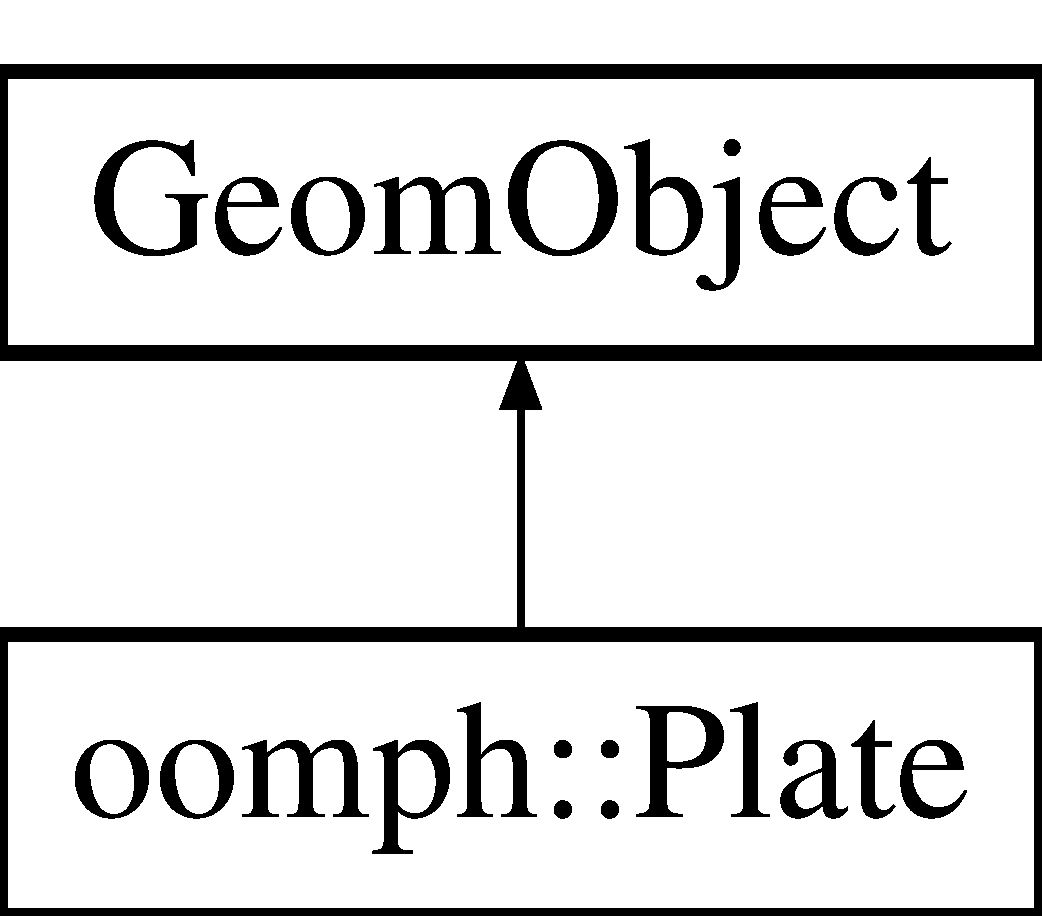
\includegraphics[height=2.000000cm]{classoomph_1_1Plate}
\end{center}
\end{figure}
\subsection*{Public Member Functions}
\begin{DoxyCompactItemize}
\item 
\hyperlink{classoomph_1_1Plate_a61811f7521511ed6e82758d050fa8d69}{Plate} (const double \&\hyperlink{classoomph_1_1Plate_a5bf44a99e0504b4c1185656d6b1b9740}{a}, const double \&\hyperlink{classoomph_1_1Plate_a24a8bd078b3b675c97203ba6cfa6119b}{b})
\begin{DoxyCompactList}\small\item\em Constructor\+: Specify radius. \end{DoxyCompactList}\item 
\hyperlink{classoomph_1_1Plate_a18b86a428438bed97cb98e9e138b9404}{Plate} (const \hyperlink{classoomph_1_1Plate}{Plate} \&node)
\begin{DoxyCompactList}\small\item\em Broken copy constructor. \end{DoxyCompactList}\item 
void \hyperlink{classoomph_1_1Plate_aaa31862fcb1a579c95035cfeca7f8e7e}{operator=} (const \hyperlink{classoomph_1_1Plate}{Plate} \&)
\begin{DoxyCompactList}\small\item\em Broken assignment operator. \end{DoxyCompactList}\item 
double \& \hyperlink{classoomph_1_1Plate_a5bf44a99e0504b4c1185656d6b1b9740}{a} ()
\begin{DoxyCompactList}\small\item\em Access function to x-\/half axis. \end{DoxyCompactList}\item 
double \& \hyperlink{classoomph_1_1Plate_a24a8bd078b3b675c97203ba6cfa6119b}{b} ()
\begin{DoxyCompactList}\small\item\em Access function to y-\/half axis. \end{DoxyCompactList}\item 
void \hyperlink{classoomph_1_1Plate_ad443e4bfc90da07a5d32083d341586dc}{position} (const Vector$<$ double $>$ \&zeta, Vector$<$ double $>$ \&r) const
\begin{DoxyCompactList}\small\item\em Position vector. \end{DoxyCompactList}\item 
virtual unsigned \hyperlink{classoomph_1_1Plate_a495af9d0abd0af9a9f25ac3bfa4820e4}{ngeom\+\_\+data} () const
\begin{DoxyCompactList}\small\item\em How many items of Data does the shape of the object depend on? \end{DoxyCompactList}\item 
void \hyperlink{classoomph_1_1Plate_ac44838098ef36d9400c534252579d6e4}{d2position} (const Vector$<$ double $>$ \&zeta, Rank\+Three\+Tensor$<$ double $>$ \&ddrdzeta) const
\begin{DoxyCompactList}\small\item\em Position Vector and 1st and 2nd derivs w.\+r.\+t. zeta. \end{DoxyCompactList}\item 
void \hyperlink{classoomph_1_1Plate_ad3f465392d03904976c58c1d55c7d6cc}{d2position} (const Vector$<$ double $>$ \&zeta, Vector$<$ double $>$ \&r, Dense\+Matrix$<$ double $>$ \&drdzeta, Rank\+Three\+Tensor$<$ double $>$ \&ddrdzeta) const
\begin{DoxyCompactList}\small\item\em Position Vector and 1st and 2nd derivs w.\+r.\+t. zeta. \end{DoxyCompactList}\end{DoxyCompactItemize}
\subsection*{Private Attributes}
\begin{DoxyCompactItemize}
\item 
double \hyperlink{classoomph_1_1Plate_a482d24b39713ccb85e6e8cf7ce942c42}{A}
\begin{DoxyCompactList}\small\item\em x-\/half axis \end{DoxyCompactList}\item 
double \hyperlink{classoomph_1_1Plate_a4e549830e4d7c76536cf4140220313f2}{B}
\begin{DoxyCompactList}\small\item\em x-\/half axis \end{DoxyCompactList}\end{DoxyCompactItemize}


\subsection{Detailed Description}
Elliptical tube with half axes a and b. 

\[ {\bf r} = ( a \cos(\zeta_1), b \sin(zeta_1), \zeta_0)^T \] 

Definition at line 69 of file unstructured\+\_\+clamped\+\_\+square\+\_\+plate.\+cc.



\subsection{Constructor \& Destructor Documentation}
\mbox{\Hypertarget{classoomph_1_1Plate_a61811f7521511ed6e82758d050fa8d69}\label{classoomph_1_1Plate_a61811f7521511ed6e82758d050fa8d69}} 
\index{oomph\+::\+Plate@{oomph\+::\+Plate}!Plate@{Plate}}
\index{Plate@{Plate}!oomph\+::\+Plate@{oomph\+::\+Plate}}
\subsubsection{\texorpdfstring{Plate()}{Plate()}\hspace{0.1cm}{\footnotesize\ttfamily [1/2]}}
{\footnotesize\ttfamily oomph\+::\+Plate\+::\+Plate (\begin{DoxyParamCaption}\item[{const double \&}]{a,  }\item[{const double \&}]{b }\end{DoxyParamCaption})\hspace{0.3cm}{\ttfamily [inline]}}



Constructor\+: Specify radius. 



Definition at line 74 of file unstructured\+\_\+clamped\+\_\+square\+\_\+plate.\+cc.

\mbox{\Hypertarget{classoomph_1_1Plate_a18b86a428438bed97cb98e9e138b9404}\label{classoomph_1_1Plate_a18b86a428438bed97cb98e9e138b9404}} 
\index{oomph\+::\+Plate@{oomph\+::\+Plate}!Plate@{Plate}}
\index{Plate@{Plate}!oomph\+::\+Plate@{oomph\+::\+Plate}}
\subsubsection{\texorpdfstring{Plate()}{Plate()}\hspace{0.1cm}{\footnotesize\ttfamily [2/2]}}
{\footnotesize\ttfamily oomph\+::\+Plate\+::\+Plate (\begin{DoxyParamCaption}\item[{const \hyperlink{classoomph_1_1Plate}{Plate} \&}]{node }\end{DoxyParamCaption})\hspace{0.3cm}{\ttfamily [inline]}}



Broken copy constructor. 



Definition at line 78 of file unstructured\+\_\+clamped\+\_\+square\+\_\+plate.\+cc.



\subsection{Member Function Documentation}
\mbox{\Hypertarget{classoomph_1_1Plate_a5bf44a99e0504b4c1185656d6b1b9740}\label{classoomph_1_1Plate_a5bf44a99e0504b4c1185656d6b1b9740}} 
\index{oomph\+::\+Plate@{oomph\+::\+Plate}!a@{a}}
\index{a@{a}!oomph\+::\+Plate@{oomph\+::\+Plate}}
\subsubsection{\texorpdfstring{a()}{a()}}
{\footnotesize\ttfamily double\& oomph\+::\+Plate\+::a (\begin{DoxyParamCaption}{ }\end{DoxyParamCaption})\hspace{0.3cm}{\ttfamily [inline]}}



Access function to x-\/half axis. 



Definition at line 90 of file unstructured\+\_\+clamped\+\_\+square\+\_\+plate.\+cc.

\mbox{\Hypertarget{classoomph_1_1Plate_a24a8bd078b3b675c97203ba6cfa6119b}\label{classoomph_1_1Plate_a24a8bd078b3b675c97203ba6cfa6119b}} 
\index{oomph\+::\+Plate@{oomph\+::\+Plate}!b@{b}}
\index{b@{b}!oomph\+::\+Plate@{oomph\+::\+Plate}}
\subsubsection{\texorpdfstring{b()}{b()}}
{\footnotesize\ttfamily double\& oomph\+::\+Plate\+::b (\begin{DoxyParamCaption}{ }\end{DoxyParamCaption})\hspace{0.3cm}{\ttfamily [inline]}}



Access function to y-\/half axis. 



Definition at line 93 of file unstructured\+\_\+clamped\+\_\+square\+\_\+plate.\+cc.

\mbox{\Hypertarget{classoomph_1_1Plate_ac44838098ef36d9400c534252579d6e4}\label{classoomph_1_1Plate_ac44838098ef36d9400c534252579d6e4}} 
\index{oomph\+::\+Plate@{oomph\+::\+Plate}!d2position@{d2position}}
\index{d2position@{d2position}!oomph\+::\+Plate@{oomph\+::\+Plate}}
\subsubsection{\texorpdfstring{d2position()}{d2position()}\hspace{0.1cm}{\footnotesize\ttfamily [1/2]}}
{\footnotesize\ttfamily void oomph\+::\+Plate\+::d2position (\begin{DoxyParamCaption}\item[{const Vector$<$ double $>$ \&}]{zeta,  }\item[{Rank\+Three\+Tensor$<$ double $>$ \&}]{ddrdzeta }\end{DoxyParamCaption}) const\hspace{0.3cm}{\ttfamily [inline]}}



Position Vector and 1st and 2nd derivs w.\+r.\+t. zeta. 



Definition at line 110 of file unstructured\+\_\+clamped\+\_\+square\+\_\+plate.\+cc.

\mbox{\Hypertarget{classoomph_1_1Plate_ad3f465392d03904976c58c1d55c7d6cc}\label{classoomph_1_1Plate_ad3f465392d03904976c58c1d55c7d6cc}} 
\index{oomph\+::\+Plate@{oomph\+::\+Plate}!d2position@{d2position}}
\index{d2position@{d2position}!oomph\+::\+Plate@{oomph\+::\+Plate}}
\subsubsection{\texorpdfstring{d2position()}{d2position()}\hspace{0.1cm}{\footnotesize\ttfamily [2/2]}}
{\footnotesize\ttfamily void oomph\+::\+Plate\+::d2position (\begin{DoxyParamCaption}\item[{const Vector$<$ double $>$ \&}]{zeta,  }\item[{Vector$<$ double $>$ \&}]{r,  }\item[{Dense\+Matrix$<$ double $>$ \&}]{drdzeta,  }\item[{Rank\+Three\+Tensor$<$ double $>$ \&}]{ddrdzeta }\end{DoxyParamCaption}) const\hspace{0.3cm}{\ttfamily [inline]}}



Position Vector and 1st and 2nd derivs w.\+r.\+t. zeta. 



Definition at line 127 of file unstructured\+\_\+clamped\+\_\+square\+\_\+plate.\+cc.

\mbox{\Hypertarget{classoomph_1_1Plate_a495af9d0abd0af9a9f25ac3bfa4820e4}\label{classoomph_1_1Plate_a495af9d0abd0af9a9f25ac3bfa4820e4}} 
\index{oomph\+::\+Plate@{oomph\+::\+Plate}!ngeom\+\_\+data@{ngeom\+\_\+data}}
\index{ngeom\+\_\+data@{ngeom\+\_\+data}!oomph\+::\+Plate@{oomph\+::\+Plate}}
\subsubsection{\texorpdfstring{ngeom\+\_\+data()}{ngeom\_data()}}
{\footnotesize\ttfamily virtual unsigned oomph\+::\+Plate\+::ngeom\+\_\+data (\begin{DoxyParamCaption}{ }\end{DoxyParamCaption}) const\hspace{0.3cm}{\ttfamily [inline]}, {\ttfamily [virtual]}}



How many items of Data does the shape of the object depend on? 



Definition at line 104 of file unstructured\+\_\+clamped\+\_\+square\+\_\+plate.\+cc.

\mbox{\Hypertarget{classoomph_1_1Plate_aaa31862fcb1a579c95035cfeca7f8e7e}\label{classoomph_1_1Plate_aaa31862fcb1a579c95035cfeca7f8e7e}} 
\index{oomph\+::\+Plate@{oomph\+::\+Plate}!operator=@{operator=}}
\index{operator=@{operator=}!oomph\+::\+Plate@{oomph\+::\+Plate}}
\subsubsection{\texorpdfstring{operator=()}{operator=()}}
{\footnotesize\ttfamily void oomph\+::\+Plate\+::operator= (\begin{DoxyParamCaption}\item[{const \hyperlink{classoomph_1_1Plate}{Plate} \&}]{ }\end{DoxyParamCaption})\hspace{0.3cm}{\ttfamily [inline]}}



Broken assignment operator. 



Definition at line 84 of file unstructured\+\_\+clamped\+\_\+square\+\_\+plate.\+cc.

\mbox{\Hypertarget{classoomph_1_1Plate_ad443e4bfc90da07a5d32083d341586dc}\label{classoomph_1_1Plate_ad443e4bfc90da07a5d32083d341586dc}} 
\index{oomph\+::\+Plate@{oomph\+::\+Plate}!position@{position}}
\index{position@{position}!oomph\+::\+Plate@{oomph\+::\+Plate}}
\subsubsection{\texorpdfstring{position()}{position()}}
{\footnotesize\ttfamily void oomph\+::\+Plate\+::position (\begin{DoxyParamCaption}\item[{const Vector$<$ double $>$ \&}]{zeta,  }\item[{Vector$<$ double $>$ \&}]{r }\end{DoxyParamCaption}) const\hspace{0.3cm}{\ttfamily [inline]}}



Position vector. 



Definition at line 96 of file unstructured\+\_\+clamped\+\_\+square\+\_\+plate.\+cc.



\subsection{Member Data Documentation}
\mbox{\Hypertarget{classoomph_1_1Plate_a482d24b39713ccb85e6e8cf7ce942c42}\label{classoomph_1_1Plate_a482d24b39713ccb85e6e8cf7ce942c42}} 
\index{oomph\+::\+Plate@{oomph\+::\+Plate}!A@{A}}
\index{A@{A}!oomph\+::\+Plate@{oomph\+::\+Plate}}
\subsubsection{\texorpdfstring{A}{A}}
{\footnotesize\ttfamily double oomph\+::\+Plate\+::A\hspace{0.3cm}{\ttfamily [private]}}



x-\/half axis 



Definition at line 164 of file unstructured\+\_\+clamped\+\_\+square\+\_\+plate.\+cc.

\mbox{\Hypertarget{classoomph_1_1Plate_a4e549830e4d7c76536cf4140220313f2}\label{classoomph_1_1Plate_a4e549830e4d7c76536cf4140220313f2}} 
\index{oomph\+::\+Plate@{oomph\+::\+Plate}!B@{B}}
\index{B@{B}!oomph\+::\+Plate@{oomph\+::\+Plate}}
\subsubsection{\texorpdfstring{B}{B}}
{\footnotesize\ttfamily double oomph\+::\+Plate\+::B\hspace{0.3cm}{\ttfamily [private]}}



x-\/half axis 



Definition at line 167 of file unstructured\+\_\+clamped\+\_\+square\+\_\+plate.\+cc.



The documentation for this class was generated from the following file\+:\begin{DoxyCompactItemize}
\item 
\hyperlink{unstructured__clamped__square__plate_8cc}{unstructured\+\_\+clamped\+\_\+square\+\_\+plate.\+cc}\end{DoxyCompactItemize}

\hypertarget{classPlateProblem}{}\section{Plate\+Problem$<$ E\+L\+E\+M\+E\+NT $>$ Class Template Reference}
\label{classPlateProblem}\index{Plate\+Problem$<$ E\+L\+E\+M\+E\+N\+T $>$@{Plate\+Problem$<$ E\+L\+E\+M\+E\+N\+T $>$}}
Inheritance diagram for Plate\+Problem$<$ E\+L\+E\+M\+E\+NT $>$\+:\begin{figure}[H]
\begin{center}
\leavevmode
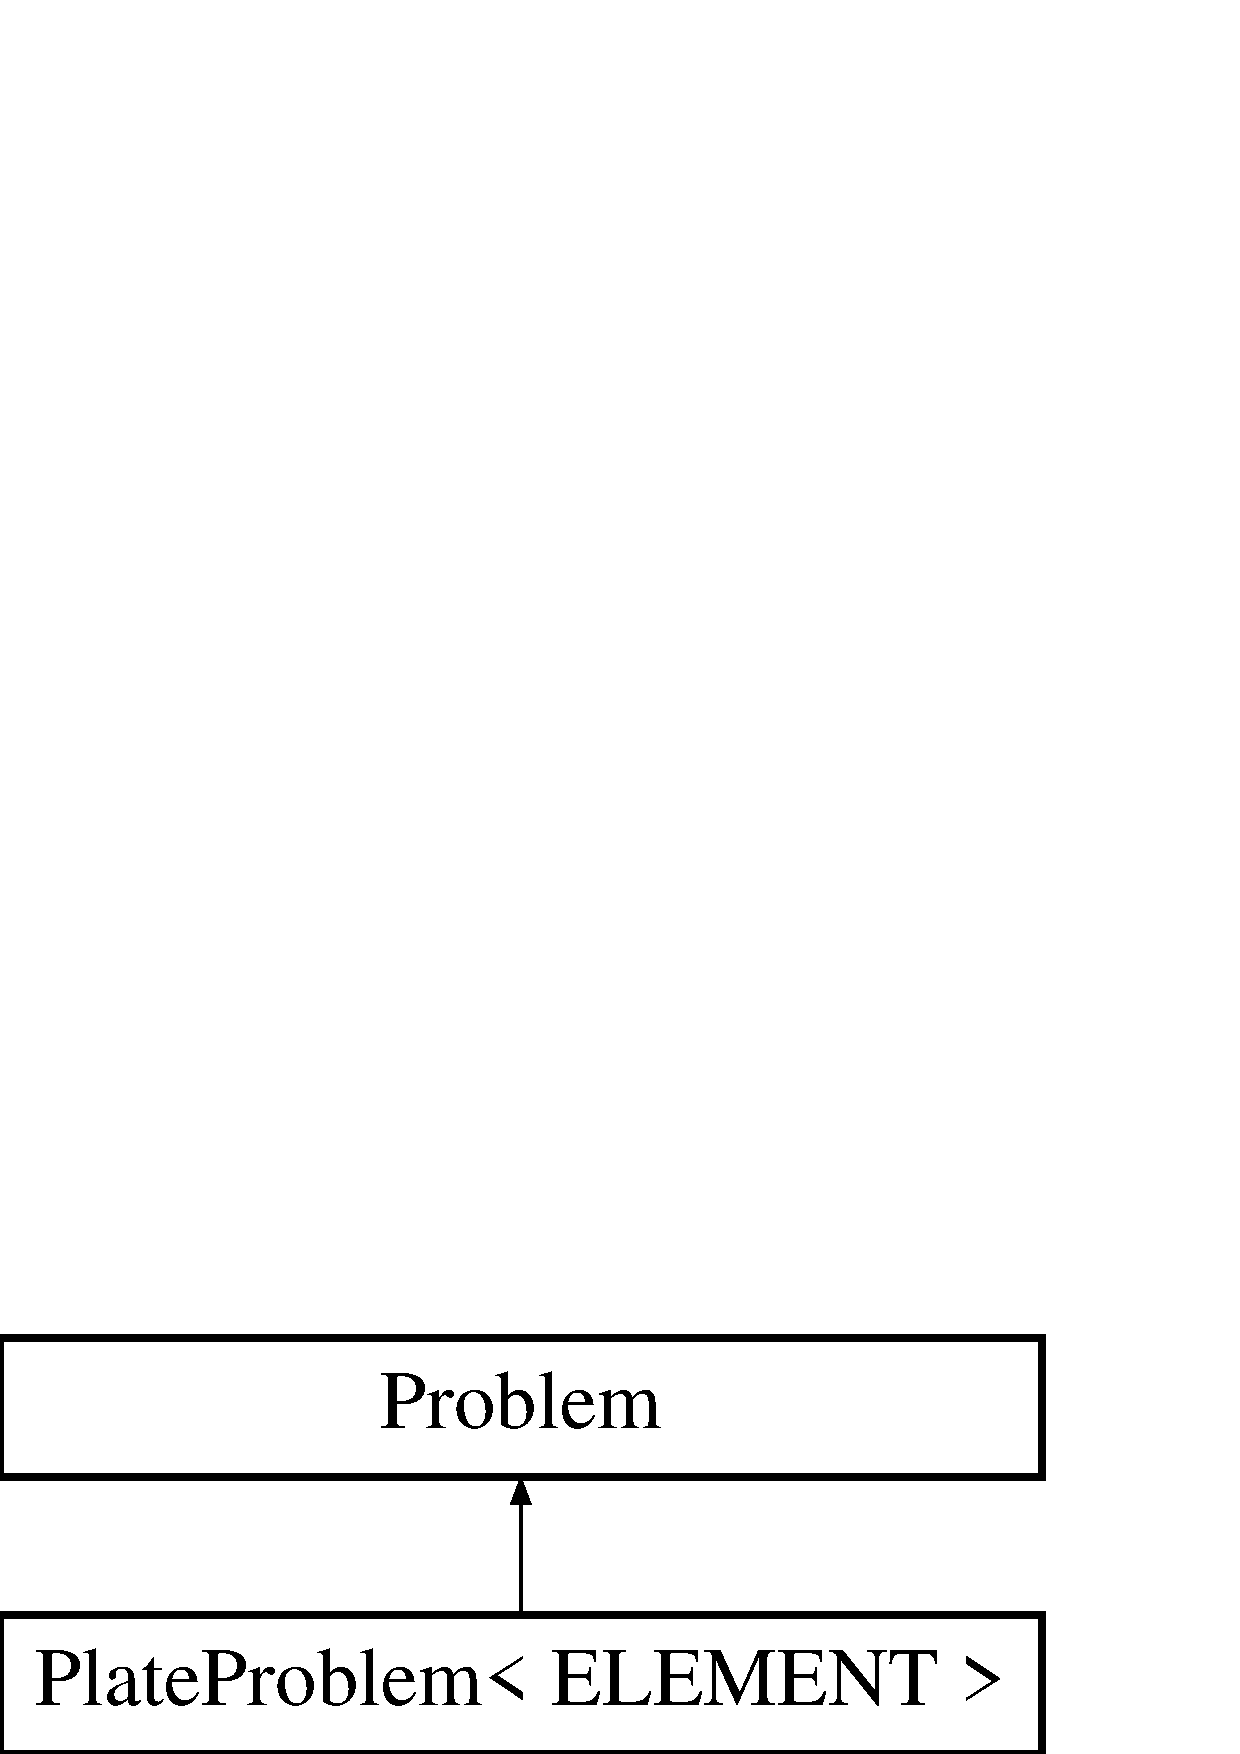
\includegraphics[height=2.000000cm]{classPlateProblem}
\end{center}
\end{figure}
\subsection*{Public Member Functions}
\begin{DoxyCompactItemize}
\item 
\hyperlink{classPlateProblem_a0430a872a8929fcda9bb205d0e69fabb}{Plate\+Problem} (const unsigned \&nx, const unsigned \&ny, const double \&lx, const double \&ly)
\begin{DoxyCompactList}\small\item\em Constructor. \end{DoxyCompactList}\item 
\hyperlink{classFlatPlateMesh}{Flat\+Plate\+Mesh}$<$ E\+L\+E\+M\+E\+NT $>$ $\ast$ \hyperlink{classPlateProblem_a964d7f9dec01b2d907fa7f3005418fcf}{mesh\+\_\+pt} ()
\begin{DoxyCompactList}\small\item\em Overload Access function for the mesh. \end{DoxyCompactList}\item 
void \hyperlink{classPlateProblem_aef1dfbdffcee81632af385733cb534f7}{actions\+\_\+after\+\_\+newton\+\_\+solve} ()
\begin{DoxyCompactList}\small\item\em Actions after solve empty. \end{DoxyCompactList}\item 
void \hyperlink{classPlateProblem_a3be5bbf9e7473c75b8f752e0d77f5955}{actions\+\_\+before\+\_\+newton\+\_\+solve} ()
\begin{DoxyCompactList}\small\item\em Actions before solve empty. \end{DoxyCompactList}\end{DoxyCompactItemize}
\subsection*{Private Attributes}
\begin{DoxyCompactItemize}
\item 
Geom\+Object $\ast$ \hyperlink{classPlateProblem_aca229d8f14f7cf1fe21fe936db72dbc2}{Undeformed\+\_\+midplane\+\_\+pt}
\begin{DoxyCompactList}\small\item\em Pointer to Geom\+Object that specifies the undeformed midplane. \end{DoxyCompactList}\item 
Node $\ast$ \hyperlink{classPlateProblem_a376d88f920e7bd37f22c7835bae5d837}{Trace\+\_\+node\+\_\+pt}
\begin{DoxyCompactList}\small\item\em First trace node. \end{DoxyCompactList}\item 
Node $\ast$ \hyperlink{classPlateProblem_afdefc2caa57f4c3fe62c05a04fe330c1}{Trace\+\_\+node2\+\_\+pt}
\begin{DoxyCompactList}\small\item\em Second trace node. \end{DoxyCompactList}\item 
unsigned \hyperlink{classPlateProblem_a6e6ae2cacb761fd29c738e7ffe54a2d0}{Nshell}
\begin{DoxyCompactList}\small\item\em Number of shell elements. \end{DoxyCompactList}\end{DoxyCompactItemize}


\subsection{Detailed Description}
\subsubsection*{template$<$class E\+L\+E\+M\+E\+NT$>$\newline
class Plate\+Problem$<$ E\+L\+E\+M\+E\+N\+T $>$}



Definition at line 318 of file plate.\+cc.



\subsection{Constructor \& Destructor Documentation}
\mbox{\Hypertarget{classPlateProblem_a0430a872a8929fcda9bb205d0e69fabb}\label{classPlateProblem_a0430a872a8929fcda9bb205d0e69fabb}} 
\index{Plate\+Problem@{Plate\+Problem}!Plate\+Problem@{Plate\+Problem}}
\index{Plate\+Problem@{Plate\+Problem}!Plate\+Problem@{Plate\+Problem}}
\subsubsection{\texorpdfstring{Plate\+Problem()}{PlateProblem()}}
{\footnotesize\ttfamily template$<$class E\+L\+E\+M\+E\+NT $>$ \\
\hyperlink{classPlateProblem}{Plate\+Problem}$<$ E\+L\+E\+M\+E\+NT $>$\+::\hyperlink{classPlateProblem}{Plate\+Problem} (\begin{DoxyParamCaption}\item[{const unsigned \&}]{nx,  }\item[{const unsigned \&}]{ny,  }\item[{const double \&}]{lx,  }\item[{const double \&}]{ly }\end{DoxyParamCaption})}



Constructor. 



Definition at line 361 of file plate.\+cc.



References Flat\+Plate\+Mesh$<$ E\+L\+E\+M\+E\+N\+T $>$\+::assign\+\_\+undeformed\+\_\+positions(), Global\+\_\+\+Physical\+\_\+\+Variables\+::H, Global\+\_\+\+Physical\+\_\+\+Variables\+::\+Nu, Global\+\_\+\+Physical\+\_\+\+Variables\+::\+Pext\+\_\+data\+\_\+pt, Global\+\_\+\+Physical\+\_\+\+Variables\+::\+Prescribed\+\_\+z, Global\+\_\+\+Physical\+\_\+\+Variables\+::press\+\_\+load(), and Global\+\_\+\+Physical\+\_\+\+Variables\+::\+Sigma0.



\subsection{Member Function Documentation}
\mbox{\Hypertarget{classPlateProblem_aef1dfbdffcee81632af385733cb534f7}\label{classPlateProblem_aef1dfbdffcee81632af385733cb534f7}} 
\index{Plate\+Problem@{Plate\+Problem}!actions\+\_\+after\+\_\+newton\+\_\+solve@{actions\+\_\+after\+\_\+newton\+\_\+solve}}
\index{actions\+\_\+after\+\_\+newton\+\_\+solve@{actions\+\_\+after\+\_\+newton\+\_\+solve}!Plate\+Problem@{Plate\+Problem}}
\subsubsection{\texorpdfstring{actions\+\_\+after\+\_\+newton\+\_\+solve()}{actions\_after\_newton\_solve()}}
{\footnotesize\ttfamily template$<$class E\+L\+E\+M\+E\+NT$>$ \\
void \hyperlink{classPlateProblem}{Plate\+Problem}$<$ E\+L\+E\+M\+E\+NT $>$\+::actions\+\_\+after\+\_\+newton\+\_\+solve (\begin{DoxyParamCaption}{ }\end{DoxyParamCaption})\hspace{0.3cm}{\ttfamily [inline]}}



Actions after solve empty. 



Definition at line 334 of file plate.\+cc.

\mbox{\Hypertarget{classPlateProblem_a3be5bbf9e7473c75b8f752e0d77f5955}\label{classPlateProblem_a3be5bbf9e7473c75b8f752e0d77f5955}} 
\index{Plate\+Problem@{Plate\+Problem}!actions\+\_\+before\+\_\+newton\+\_\+solve@{actions\+\_\+before\+\_\+newton\+\_\+solve}}
\index{actions\+\_\+before\+\_\+newton\+\_\+solve@{actions\+\_\+before\+\_\+newton\+\_\+solve}!Plate\+Problem@{Plate\+Problem}}
\subsubsection{\texorpdfstring{actions\+\_\+before\+\_\+newton\+\_\+solve()}{actions\_before\_newton\_solve()}}
{\footnotesize\ttfamily template$<$class E\+L\+E\+M\+E\+NT$>$ \\
void \hyperlink{classPlateProblem}{Plate\+Problem}$<$ E\+L\+E\+M\+E\+NT $>$\+::actions\+\_\+before\+\_\+newton\+\_\+solve (\begin{DoxyParamCaption}{ }\end{DoxyParamCaption})\hspace{0.3cm}{\ttfamily [inline]}}



Actions before solve empty. 



Definition at line 337 of file plate.\+cc.

\mbox{\Hypertarget{classPlateProblem_a964d7f9dec01b2d907fa7f3005418fcf}\label{classPlateProblem_a964d7f9dec01b2d907fa7f3005418fcf}} 
\index{Plate\+Problem@{Plate\+Problem}!mesh\+\_\+pt@{mesh\+\_\+pt}}
\index{mesh\+\_\+pt@{mesh\+\_\+pt}!Plate\+Problem@{Plate\+Problem}}
\subsubsection{\texorpdfstring{mesh\+\_\+pt()}{mesh\_pt()}}
{\footnotesize\ttfamily template$<$class E\+L\+E\+M\+E\+NT$>$ \\
\hyperlink{classFlatPlateMesh}{Flat\+Plate\+Mesh}$<$E\+L\+E\+M\+E\+NT$>$$\ast$ \hyperlink{classPlateProblem}{Plate\+Problem}$<$ E\+L\+E\+M\+E\+NT $>$\+::mesh\+\_\+pt (\begin{DoxyParamCaption}{ }\end{DoxyParamCaption})\hspace{0.3cm}{\ttfamily [inline]}}



Overload Access function for the mesh. 



Definition at line 328 of file plate.\+cc.



Referenced by main().



\subsection{Member Data Documentation}
\mbox{\Hypertarget{classPlateProblem_a6e6ae2cacb761fd29c738e7ffe54a2d0}\label{classPlateProblem_a6e6ae2cacb761fd29c738e7ffe54a2d0}} 
\index{Plate\+Problem@{Plate\+Problem}!Nshell@{Nshell}}
\index{Nshell@{Nshell}!Plate\+Problem@{Plate\+Problem}}
\subsubsection{\texorpdfstring{Nshell}{Nshell}}
{\footnotesize\ttfamily template$<$class E\+L\+E\+M\+E\+NT$>$ \\
unsigned \hyperlink{classPlateProblem}{Plate\+Problem}$<$ E\+L\+E\+M\+E\+NT $>$\+::Nshell\hspace{0.3cm}{\ttfamily [private]}}



Number of shell elements. 



Definition at line 351 of file plate.\+cc.

\mbox{\Hypertarget{classPlateProblem_afdefc2caa57f4c3fe62c05a04fe330c1}\label{classPlateProblem_afdefc2caa57f4c3fe62c05a04fe330c1}} 
\index{Plate\+Problem@{Plate\+Problem}!Trace\+\_\+node2\+\_\+pt@{Trace\+\_\+node2\+\_\+pt}}
\index{Trace\+\_\+node2\+\_\+pt@{Trace\+\_\+node2\+\_\+pt}!Plate\+Problem@{Plate\+Problem}}
\subsubsection{\texorpdfstring{Trace\+\_\+node2\+\_\+pt}{Trace\_node2\_pt}}
{\footnotesize\ttfamily template$<$class E\+L\+E\+M\+E\+NT$>$ \\
Node$\ast$ \hyperlink{classPlateProblem}{Plate\+Problem}$<$ E\+L\+E\+M\+E\+NT $>$\+::Trace\+\_\+node2\+\_\+pt\hspace{0.3cm}{\ttfamily [private]}}



Second trace node. 



Definition at line 348 of file plate.\+cc.

\mbox{\Hypertarget{classPlateProblem_a376d88f920e7bd37f22c7835bae5d837}\label{classPlateProblem_a376d88f920e7bd37f22c7835bae5d837}} 
\index{Plate\+Problem@{Plate\+Problem}!Trace\+\_\+node\+\_\+pt@{Trace\+\_\+node\+\_\+pt}}
\index{Trace\+\_\+node\+\_\+pt@{Trace\+\_\+node\+\_\+pt}!Plate\+Problem@{Plate\+Problem}}
\subsubsection{\texorpdfstring{Trace\+\_\+node\+\_\+pt}{Trace\_node\_pt}}
{\footnotesize\ttfamily template$<$class E\+L\+E\+M\+E\+NT$>$ \\
Node$\ast$ \hyperlink{classPlateProblem}{Plate\+Problem}$<$ E\+L\+E\+M\+E\+NT $>$\+::Trace\+\_\+node\+\_\+pt\hspace{0.3cm}{\ttfamily [private]}}



First trace node. 



Definition at line 345 of file plate.\+cc.

\mbox{\Hypertarget{classPlateProblem_aca229d8f14f7cf1fe21fe936db72dbc2}\label{classPlateProblem_aca229d8f14f7cf1fe21fe936db72dbc2}} 
\index{Plate\+Problem@{Plate\+Problem}!Undeformed\+\_\+midplane\+\_\+pt@{Undeformed\+\_\+midplane\+\_\+pt}}
\index{Undeformed\+\_\+midplane\+\_\+pt@{Undeformed\+\_\+midplane\+\_\+pt}!Plate\+Problem@{Plate\+Problem}}
\subsubsection{\texorpdfstring{Undeformed\+\_\+midplane\+\_\+pt}{Undeformed\_midplane\_pt}}
{\footnotesize\ttfamily template$<$class E\+L\+E\+M\+E\+NT$>$ \\
Geom\+Object$\ast$ \hyperlink{classPlateProblem}{Plate\+Problem}$<$ E\+L\+E\+M\+E\+NT $>$\+::Undeformed\+\_\+midplane\+\_\+pt\hspace{0.3cm}{\ttfamily [private]}}



Pointer to Geom\+Object that specifies the undeformed midplane. 



Definition at line 342 of file plate.\+cc.



The documentation for this class was generated from the following file\+:\begin{DoxyCompactItemize}
\item 
\hyperlink{plate_8cc}{plate.\+cc}\end{DoxyCompactItemize}

\chapter{File Documentation}
\hypertarget{linear__shell_8txt__doxygenified_8h}{}\section{linear\+\_\+shell.\+txt\+\_\+doxygenified.\+h File Reference}
\label{linear__shell_8txt__doxygenified_8h}\index{linear\+\_\+shell.\+txt\+\_\+doxygenified.\+h@{linear\+\_\+shell.\+txt\+\_\+doxygenified.\+h}}

\hypertarget{plate_8cc}{}\section{plate.\+cc File Reference}
\label{plate_8cc}\index{plate.\+cc@{plate.\+cc}}
{\ttfamily \#include \char`\"{}generic.\+h\char`\"{}}\newline
{\ttfamily \#include \char`\"{}shell.\+h\char`\"{}}\newline
{\ttfamily \#include \char`\"{}meshes/rectangular\+\_\+quadmesh.\+h\char`\"{}}\newline
\subsection*{Classes}
\begin{DoxyCompactItemize}
\item 
class \hyperlink{classFlatPlate}{Flat\+Plate}
\begin{DoxyCompactList}\small\item\em Flat plate in x-\/y plane. \end{DoxyCompactList}\item 
class \hyperlink{classFlatPlateMesh}{Flat\+Plate\+Mesh$<$ E\+L\+E\+M\+E\+N\+T $>$}
\item 
class \hyperlink{classPlateProblem}{Plate\+Problem$<$ E\+L\+E\+M\+E\+N\+T $>$}
\end{DoxyCompactItemize}
\subsection*{Namespaces}
\begin{DoxyCompactItemize}
\item 
 \hyperlink{namespaceGlobal__Physical__Variables}{Global\+\_\+\+Physical\+\_\+\+Variables}
\begin{DoxyCompactList}\small\item\em Global variables that represent physical properties. \end{DoxyCompactList}\end{DoxyCompactItemize}
\subsection*{Functions}
\begin{DoxyCompactItemize}
\item 
double \hyperlink{namespaceGlobal__Physical__Variables_a80149b39ce76ea0a779f7493905eb1b8}{Global\+\_\+\+Physical\+\_\+\+Variables\+::external\+\_\+pressure} ()
\begin{DoxyCompactList}\small\item\em Return a reference to the external pressure load on the elastic tube. \end{DoxyCompactList}\item 
void \hyperlink{namespaceGlobal__Physical__Variables_a86fd8f502cb8c4c7939ffae742f023eb}{Global\+\_\+\+Physical\+\_\+\+Variables\+::press\+\_\+load} (const Vector$<$ double $>$ \&xi, const Vector$<$ double $>$ \&x, const Vector$<$ double $>$ \&N, Vector$<$ double $>$ \&load)
\begin{DoxyCompactList}\small\item\em Load function, normal pressure loading. \end{DoxyCompactList}\item 
int \hyperlink{plate_8cc_a0ddf1224851353fc92bfbff6f499fa97}{main} (int argc, char $\ast$argv\mbox{[}$\,$\mbox{]})
\begin{DoxyCompactList}\small\item\em Driver. \end{DoxyCompactList}\end{DoxyCompactItemize}
\subsection*{Variables}
\begin{DoxyCompactItemize}
\item 
double \hyperlink{namespaceGlobal__Physical__Variables_a97964adfdf99492b01f8e0b1c4603bc8}{Global\+\_\+\+Physical\+\_\+\+Variables\+::\+Prescribed\+\_\+z} = 0.\+0
\begin{DoxyCompactList}\small\item\em Prescribed position of control point. \end{DoxyCompactList}\item 
Data $\ast$ \hyperlink{namespaceGlobal__Physical__Variables_a9d598320fb3d7ecf94101088e8f376d2}{Global\+\_\+\+Physical\+\_\+\+Variables\+::\+Pext\+\_\+data\+\_\+pt}
\begin{DoxyCompactList}\small\item\em Pointer to pressure load (stored in Data so it can become an unknown in the problem when displacement control is used. \end{DoxyCompactList}\item 
double \hyperlink{namespaceGlobal__Physical__Variables_a417dc688a70c4f06ef0faed047068ba2}{Global\+\_\+\+Physical\+\_\+\+Variables\+::\+Sigma0} =0.\+1
\begin{DoxyCompactList}\small\item\em 2nd Piola Kirchhoff pre-\/stress \end{DoxyCompactList}\item 
double \hyperlink{namespaceGlobal__Physical__Variables_a3962c36313826b19f216f6bbbdd6a477}{Global\+\_\+\+Physical\+\_\+\+Variables\+::\+Nu} =0.\+3
\begin{DoxyCompactList}\small\item\em Poisson\textquotesingle{}s ratio. \end{DoxyCompactList}\item 
double \hyperlink{namespaceGlobal__Physical__Variables_af6e07423e22c0991084d9a2f43727805}{Global\+\_\+\+Physical\+\_\+\+Variables\+::H} =0.\+01
\begin{DoxyCompactList}\small\item\em Wall thickness. \end{DoxyCompactList}\end{DoxyCompactItemize}


\subsection{Function Documentation}
\mbox{\Hypertarget{plate_8cc_a0ddf1224851353fc92bfbff6f499fa97}\label{plate_8cc_a0ddf1224851353fc92bfbff6f499fa97}} 
\index{plate.\+cc@{plate.\+cc}!main@{main}}
\index{main@{main}!plate.\+cc@{plate.\+cc}}
\subsubsection{\texorpdfstring{main()}{main()}}
{\footnotesize\ttfamily int main (\begin{DoxyParamCaption}\item[{int}]{argc,  }\item[{char $\ast$}]{argv\mbox{[}$\,$\mbox{]} }\end{DoxyParamCaption})}



Driver. 

(pow(0.\+05,3)/12.0) $<$$<$ \char`\"{} \char`\"{} 

Definition at line 555 of file plate.\+cc.



References Global\+\_\+\+Physical\+\_\+\+Variables\+::external\+\_\+pressure(), Global\+\_\+\+Physical\+\_\+\+Variables\+::H, Plate\+Problem$<$ E\+L\+E\+M\+E\+N\+T $>$\+::mesh\+\_\+pt(), Global\+\_\+\+Physical\+\_\+\+Variables\+::\+Prescribed\+\_\+z, and Global\+\_\+\+Physical\+\_\+\+Variables\+::\+Sigma0.


\hypertarget{unstructured__clamped__square__plate_8cc}{}\section{unstructured\+\_\+clamped\+\_\+square\+\_\+plate.\+cc File Reference}
\label{unstructured__clamped__square__plate_8cc}\index{unstructured\+\_\+clamped\+\_\+square\+\_\+plate.\+cc@{unstructured\+\_\+clamped\+\_\+square\+\_\+plate.\+cc}}
{\ttfamily \#include \char`\"{}generic.\+h\char`\"{}}\newline
{\ttfamily \#include \char`\"{}meshes/one\+\_\+d\+\_\+mesh.\+h\char`\"{}}\newline
{\ttfamily \#include \char`\"{}meshes/simple\+\_\+rectangular\+\_\+tri\+\_\+mesh.\+h\char`\"{}}\newline
{\ttfamily \#include \char`\"{}meshes/simple\+\_\+rectangular\+\_\+quadmesh.\+h\char`\"{}}\newline
{\ttfamily \#include \char`\"{}generic/geom\+\_\+objects.\+h\char`\"{}}\newline
{\ttfamily \#include \char`\"{}meshes/triangle\+\_\+mesh.\+h\char`\"{}}\newline
\subsection*{Classes}
\begin{DoxyCompactItemize}
\item 
class \hyperlink{classoomph_1_1Plate}{oomph\+::\+Plate}
\begin{DoxyCompactList}\small\item\em Elliptical tube with half axes a and b. \end{DoxyCompactList}\item 
class \hyperlink{classoomph_1_1MyShellEquations}{oomph\+::\+My\+Shell\+Equations$<$ D\+I\+M, N\+N\+O\+D\+E\+\_\+1\+D $>$}
\item 
class \hyperlink{classoomph_1_1BellShellElement}{oomph\+::\+Bell\+Shell\+Element$<$ D\+I\+M, N\+N\+O\+D\+E\+\_\+1\+D $>$}
\begin{DoxyCompactList}\small\item\em \hyperlink{classoomph_1_1BellShellElement}{Bell\+Shell\+Element} elements are with subparametric interpolation for the function. \end{DoxyCompactList}\item 
class \hyperlink{classoomph_1_1FaceGeometry_3_01BellShellElement_3_01DIM_00_01NNODE__1D_01_4_01_4}{oomph\+::\+Face\+Geometry$<$ Bell\+Shell\+Element$<$ D\+I\+M, N\+N\+O\+D\+E\+\_\+1\+D $>$ $>$}
\item 
class \hyperlink{classMyLinearisedShellProblem}{My\+Linearised\+Shell\+Problem$<$ E\+L\+E\+M\+E\+N\+T, D\+I\+M, N\+N\+O\+D\+E\+\_\+1\+D $>$}
\begin{DoxyCompactList}\small\item\em 2D linearised shell problem. \end{DoxyCompactList}\end{DoxyCompactItemize}
\subsection*{Namespaces}
\begin{DoxyCompactItemize}
\item 
 \hyperlink{namespaceoomph}{oomph}
\item 
 \hyperlink{namespacePhysical__Variables}{Physical\+\_\+\+Variables}
\begin{DoxyCompactList}\small\item\em Namespace for the solution of 2D linear shell equation. \end{DoxyCompactList}\end{DoxyCompactItemize}
\subsection*{Macros}
\begin{DoxyCompactItemize}
\item 
\#define \hyperlink{unstructured__clamped__square__plate_8cc_acfe9945021d2478e31287c08a1be3a89}{O\+O\+M\+P\+H\+\_\+\+L\+I\+N\+E\+A\+R\+\_\+\+S\+H\+E\+L\+L\+\_\+\+E\+L\+E\+M\+E\+N\+T\+S\+\_\+\+H\+E\+A\+D\+ER}
\end{DoxyCompactItemize}
\subsection*{Functions}
\begin{DoxyCompactItemize}
\item 
void \hyperlink{namespacePhysical__Variables_af90d0c580c57b1152fd1cc7046055031}{Physical\+\_\+\+Variables\+::get\+\_\+exact\+\_\+u} (const Vector$<$ double $>$ \&x, Vector$<$ double $>$ \&u)
\item 
void \hyperlink{namespacePhysical__Variables_a36f0d0dc5f8aa4eafd7c4d6fe943c4e8}{Physical\+\_\+\+Variables\+::source\+\_\+function} (const Vector$<$ double $>$ \&x, const Vector$<$ double $>$ \&unit\+\_\+n, Vector$<$ double $>$ \&source)
\begin{DoxyCompactList}\small\item\em Source function applied in the normal vector. \end{DoxyCompactList}\item 
int \hyperlink{unstructured__clamped__square__plate_8cc_a0ddf1224851353fc92bfbff6f499fa97}{main} (int argc, char $\ast$argv\mbox{[}$\,$\mbox{]})
\begin{DoxyCompactList}\small\item\em Driver for 2D linearised shell problem\+: square flat plate. \end{DoxyCompactList}\end{DoxyCompactItemize}
\subsection*{Variables}
\begin{DoxyCompactItemize}
\item 
double \hyperlink{namespacePhysical__Variables_a58adc76bae4751599143c613f9100904}{Physical\+\_\+\+Variables\+::\+P\+\_\+ext}
\begin{DoxyCompactList}\small\item\em Pressure load. \end{DoxyCompactList}\item 
double \hyperlink{namespacePhysical__Variables_ac374cc60da0f1e5df3fc48a3c9ce1d74}{Physical\+\_\+\+Variables\+::epsilon} = 1.\+0e-\/8
\end{DoxyCompactItemize}


\subsection{Macro Definition Documentation}
\mbox{\Hypertarget{unstructured__clamped__square__plate_8cc_acfe9945021d2478e31287c08a1be3a89}\label{unstructured__clamped__square__plate_8cc_acfe9945021d2478e31287c08a1be3a89}} 
\index{unstructured\+\_\+clamped\+\_\+square\+\_\+plate.\+cc@{unstructured\+\_\+clamped\+\_\+square\+\_\+plate.\+cc}!O\+O\+M\+P\+H\+\_\+\+L\+I\+N\+E\+A\+R\+\_\+\+S\+H\+E\+L\+L\+\_\+\+E\+L\+E\+M\+E\+N\+T\+S\+\_\+\+H\+E\+A\+D\+ER@{O\+O\+M\+P\+H\+\_\+\+L\+I\+N\+E\+A\+R\+\_\+\+S\+H\+E\+L\+L\+\_\+\+E\+L\+E\+M\+E\+N\+T\+S\+\_\+\+H\+E\+A\+D\+ER}}
\index{O\+O\+M\+P\+H\+\_\+\+L\+I\+N\+E\+A\+R\+\_\+\+S\+H\+E\+L\+L\+\_\+\+E\+L\+E\+M\+E\+N\+T\+S\+\_\+\+H\+E\+A\+D\+ER@{O\+O\+M\+P\+H\+\_\+\+L\+I\+N\+E\+A\+R\+\_\+\+S\+H\+E\+L\+L\+\_\+\+E\+L\+E\+M\+E\+N\+T\+S\+\_\+\+H\+E\+A\+D\+ER}!unstructured\+\_\+clamped\+\_\+square\+\_\+plate.\+cc@{unstructured\+\_\+clamped\+\_\+square\+\_\+plate.\+cc}}
\subsubsection{\texorpdfstring{O\+O\+M\+P\+H\+\_\+\+L\+I\+N\+E\+A\+R\+\_\+\+S\+H\+E\+L\+L\+\_\+\+E\+L\+E\+M\+E\+N\+T\+S\+\_\+\+H\+E\+A\+D\+ER}{OOMPH\_LINEAR\_SHELL\_ELEMENTS\_HEADER}}
{\footnotesize\ttfamily \#define O\+O\+M\+P\+H\+\_\+\+L\+I\+N\+E\+A\+R\+\_\+\+S\+H\+E\+L\+L\+\_\+\+E\+L\+E\+M\+E\+N\+T\+S\+\_\+\+H\+E\+A\+D\+ER}



Definition at line 52 of file unstructured\+\_\+clamped\+\_\+square\+\_\+plate.\+cc.



\subsection{Function Documentation}
\mbox{\Hypertarget{unstructured__clamped__square__plate_8cc_a0ddf1224851353fc92bfbff6f499fa97}\label{unstructured__clamped__square__plate_8cc_a0ddf1224851353fc92bfbff6f499fa97}} 
\index{unstructured\+\_\+clamped\+\_\+square\+\_\+plate.\+cc@{unstructured\+\_\+clamped\+\_\+square\+\_\+plate.\+cc}!main@{main}}
\index{main@{main}!unstructured\+\_\+clamped\+\_\+square\+\_\+plate.\+cc@{unstructured\+\_\+clamped\+\_\+square\+\_\+plate.\+cc}}
\subsubsection{\texorpdfstring{main()}{main()}}
{\footnotesize\ttfamily int main (\begin{DoxyParamCaption}\item[{int}]{argc,  }\item[{char $\ast$}]{argv\mbox{[}$\,$\mbox{]} }\end{DoxyParamCaption})}



Driver for 2D linearised shell problem\+: square flat plate. 



Definition at line 1887 of file unstructured\+\_\+clamped\+\_\+square\+\_\+plate.\+cc.



References My\+Linearised\+Shell\+Problem$<$ E\+L\+E\+M\+E\+N\+T, D\+I\+M, N\+N\+O\+D\+E\+\_\+1\+D $>$\+::parameter\+\_\+study(), and Physical\+\_\+\+Variables\+::source\+\_\+function().


%--- End generated contents ---

% Index
\backmatter
\newpage
\phantomsection
\clearemptydoublepage
\addcontentsline{toc}{chapter}{Index}
\printindex

